\documentclass[12pt,a4paper,twoside]{article}
\usepackage[margin=2cm]{geometry}
\usepackage{graphicx}
\usepackage{varioref}
\usepackage{xspace}
\usepackage{listings}
\usepackage{ifpdf}
\usepackage{hyperref}
\newcommand{\class}[1]{\texttt{\textbf{#1}}\xspace}
\newcommand{\method}[1]{\texttt{#1}\xspace}
\renewcommand{\rmdefault}{ptm}

% 
% ---------------------------------------------------------------
% define new commands/symbols
% ---------------------------------------------------------------
% 
% General stuff
% 
\hyphenation{ILC}
\hyphenation{between}
\hyphenation{basis}
\hyphenation{below}
\hyphenation{because}
\hyphenation{da-ta-ba-ses}

\newcommand{\pt}{\ensuremath{p_{\mathrm{t}}}}
\newcommand{\et}{\ensuremath{E_{\mathrm{T}}}}
\newcommand {\pT} {\mbox{$p_{\rm t}$}}
\newcommand{\mt}{\ensuremath{m_{\mathrm{t}}}}
\newcommand {\grid} {Grid\@\xspace}
\newcommand {\MC} {Monte~Carlo\@\xspace}
\newcommand {\alien} {AliEn\@\xspace}
\newcommand {\pp} {\mbox{p--p}\@\xspace} 
\newcommand {\pA} {\mbox{p--A}\@\xspace} 
\newcommand {\PbPb} {\mbox{Pb--Pb}\@\xspace}
\newcommand {\ilcroot} {IlcRoot\@\xspace}
\newcommand {\ROOT} {ROOT\@\xspace}
\newcommand {\OO} {Object-Oriented\@\xspace}

\newcommand{\mrm}{\mathrm}
\newcommand{\dd}{\mrm{d}}
\newcommand{\elm}{e.m.\@\xspace}
\newcommand{\eg}{{e.g.~\@\xspace}}
\newcommand{\ie}{i.e.\@\xspace}
\newcommand{\Jpsi} {\mbox{J\kern-0.05em /\kern-0.05em$\psi$}\xspace}
\newcommand{\psip} {\mbox{$\psi^\prime$}\xspace}
\newcommand{\Ups} {\mbox{$\Upsilon$}\xspace}
\newcommand{\Upsp} {\mbox{$\Upsilon^\prime$}\xspace}
\newcommand{\Upspp} {\mbox{$\Upsilon^{\prime\prime}$}\xspace}
\newcommand{\qqbar} {\mbox{$q\bar{q}$}\xspace}

\newcommand {\grad} {\mbox{$^{\circ}$}}

\newcommand {\rap} {\mbox{$\left | y \right | $}}
\newcommand {\mass} {\mbox{\rm GeV$\kern-0.15em /\kern-0.12em c^2$}}
\newcommand {\tev} {\mbox{${\rm TeV}$}}
\newcommand {\gev} {\mbox{${\rm GeV}$}}
\newcommand {\mev} {\mbox{${\rm MeV}$}}
\newcommand {\kev} {\mbox{${\rm keV}$}}
\newcommand {\mom} {\mbox{\rm GeV$\kern-0.15em /\kern-0.12em c$}}
\newcommand {\mum} {\mbox{$\mu {\rm m}$}}
\newcommand {\gmom} {\mbox{\rm GeV$\kern-0.15em /\kern-0.12em c$}}
\newcommand {\mmass} {\mbox{\rm MeV$\kern-0.15em /\kern-0.12em c^2$}}
\newcommand {\mmom} {\mbox{\rm MeV$\kern-0.15em /\kern-0.12em c$}}
\newcommand {\nb} {\mbox{\rm nb}}
\newcommand {\musec} {\mbox{$\mu {\rm s}$}}
\newcommand {\cmq} {\mbox{${\rm cm}^{2}$}}
\newcommand {\cm} {\mbox{${\rm cm}$}}
\newcommand {\mm} {\mbox{${\rm mm}$}}
\newcommand {\dens} {\mbox{${\rm g}\,{\rm cm}^{-3}$}}
%
\newcommand{\FR}{ILC alignment framework}
\newcommand{\tgeo}{\lstinline!TGeo!}
%
\lstset{                      % general command to set parameter(s)
%  basicstyle=\small,          % print whole listing small
  basicstyle=\ttfamily,       % print whole listing monospace
  keywordstyle=\bfseries,     % bold black keywords
  identifierstyle=,           % identifiers in itilcm
  commentstyle=\itshape,      % white comments in itilcm
  stringstyle=\ttfamily,      % typewriter type for strings
  showstringspaces=false,     % no special string spaces
  columns=fullflexible,       % Flexible columns
  xleftmargin=2em,            % Extra margin, left
  xrightmargin=2em,           % Extra margin, right
  numbers=left,               % Line numbers on the left
  numberfirstline=true,       % First line numbered
  firstnumber=1,              % Always start at 1 
  stepnumber=5,               % Every fifth line 
  numberstyle=\footnotesize\itshape, % Style of line numbers
  frame=lines}                % Lines above and below listings

% 
% ---------------------------------------------------------
% - End of Definitions
% ---------------------------------------------------------

\begin{document}

\title{IlcRoot Primer}
\author{Editor P.Hristov}
\date{Version v4-05-06 \\
22/11/2006
}

\maketitle
\tableofcontents
%\lstlistoflistings

%%%%%%%%%%%%%%%%%%%%%%%%%%%%%%%%%%%%%%%%%%%%%%%%%%%%%%%%%%%%%%%%%%%%%%%%%%%%%%%
\cleardoublepage 
\section{Introduction}\label{Introduction}

% -----------------------------------------------------------------------------


\subsection{About this primer}

The aim  of this primer  is to give  some basic information  about the
ILC offline  framework (IlcRoot) from users  perspective. We explain
in  detail  the installation  procedure,  and  give  examples of  some
typical  use cases: detector  description, event  generation, particle
transport,   generation  of   ``summable   digits'',  event   merging,
reconstruction,  particle  identification,  and  generation  of  event
summary data. The primer also  includes some examples of analysis, and
short  description of  the existing  analysis classes  in  IlcRoot. An
updated   version   of   the   document   can   be   downloaded   from
\url{http://ilcinfo.cern.ch/Offline/IlcRoot/primer.html}.

For  the reader  interested by  the  IlcRoot architecture  and by  the
performance studies done so far, a good starting point is Chapter 4 of
the  ILC  Physics  Performance Report\cite{PPR}.  Another  important
document is the ILC Computing Technical Design Report\cite{CompTDR}.
Some  information contained  there has  been included  in  the present
document, but most of the details have been omitted.

IlcRoot uses the  ROOT\cite{ROOT} system as a foundation  on which the
framework for  simulation, reconstruction  and analysis is  built. The
transport of the  particles through the detector is  carried on by the
Geant3\cite{Geant3}   or  FLUKA\cite{FLUKA}   packages.   Support  for
Geant4\cite{Geant4} transport package is coming soon.

Except for large existing libraries, such as Pythia6\cite{MC:PYTH} and
HIJING\cite{MC:HIJING}, and some remaining legacy code, this framework
is  based on  the  Object  Oriented programming  paradigm,  and it  is
written in C++.

The following packages are needed to install the fully operational
software distribution: 
\begin{itemize}
\item ROOT, available from \url{http://root.cern.ch}
or using the ROOT CVS repository
\begin{verbatim}
:pserver:cvs@root.cern.ch:/user/cvs
\end{verbatim}
\item IlcRoot from the ILC offline CVS repository 
\begin{verbatim}
:pserver:cvs@ilcsoft.cern.ch:/soft/cvsroot
\end{verbatim}
\item transport packages:
\begin{itemize}
\item GEANT~3 is available from the ROOT CVS repository
\item  FLUKA library can
be obtained after registration from \url{http://www.fluka.org}
\item GEANT~4 distribution from \url{http://cern.ch/geant4}.
\end{itemize}
\end{itemize}

The access to the GRID resources and data is provided by the
AliEn\cite{AliEn} system.

The installation details are explained in Section \ref{Installation}.

\subsection{IlcRoot framework}\label{IlcRootFramework}

In HEP, a framework is a set of software tools that enables data
processing. For example the old CERN Program Library was a toolkit to
build a framework. PAW was the first example of integration of tools
into a coherent ensemble specifically dedicated to data analysis. The
role of the framework is shown in Fig.~\ref{MC:Parab}.

\begin{figure}[ht]
  \centering
  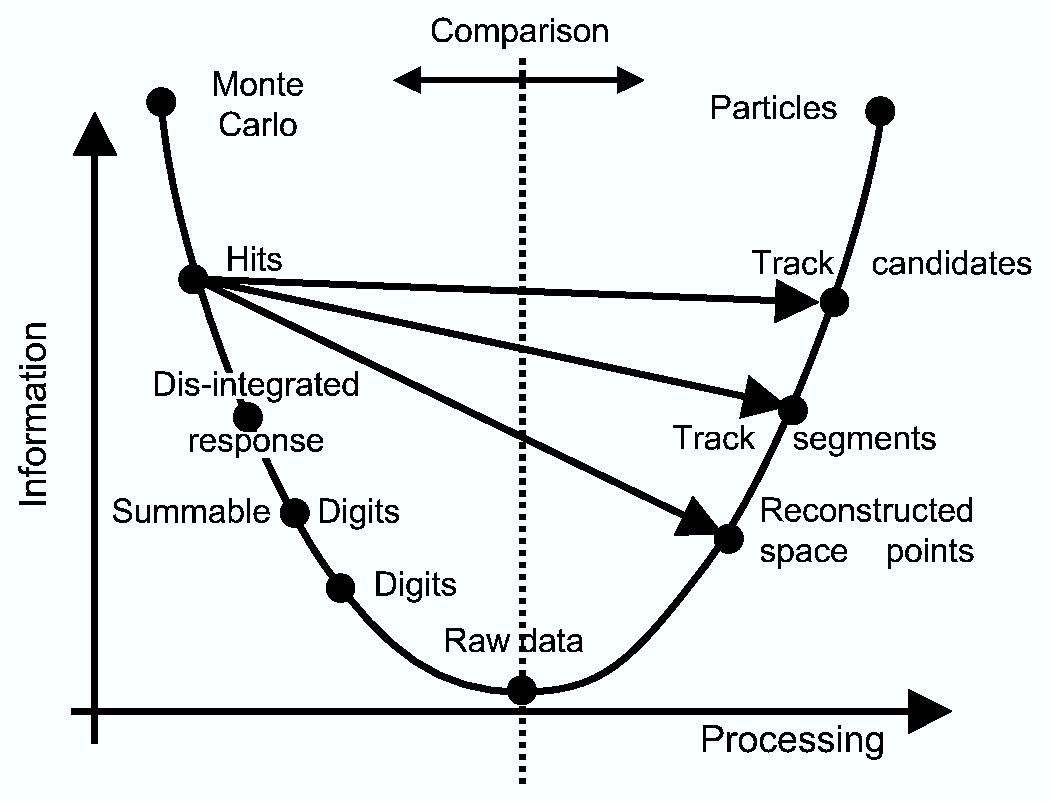
\includegraphics[width=10cm]{picts/Parab}
  \caption{Data processing framework.} \label{MC:Parab}
\end{figure}

The primary  interactions are simulated via event  generators, and the
resulting kinematic  tree is then  used in the transport  package.  An
event generator produces set  of ``particles'' with their momenta. The
set of particles, where one  maintains the production history (in form
of  mother-daughter  relationship  and  production vertex)  forms  the
kinematic tree. More details can be found in the ROOT documentation of
class  \class{TParticle}.    The  transport  package   transports  the
particles through  the set  of detectors, and  produces \textbf{hits},
which  in  ILC  terminology  means  energy  deposition  at  a  given
point. The hits contain  also information (``track labels'') about the
particles that have generated them.  In case of calorimeters (PHOS and
EMCAL) the hit is the energy  deposition in the whole active volume of
a detecting element.  In some detectors the energy of  the hit is used
only for comparison with a given threshold, for example in TOF and ITS
pixel layers.

At the next step the detector  response is taken into account, and the
hits are transformed into  \textbf{digits}. As it was explained above,
the hits are  closely related to the tracks  which generated them. The
transition  from  hits/tracks to  digits/detectors  is  marked on  the
picture    as    ``disintegrated    response'',   the    tracks    are
``disintegrated''  and  only the  labels  carry  the \MC  information.
There  are two types  of digits:  \textbf{summable digits},  where one
uses  low thresholds  and the  result is  additive, and  {\bf digits},
where the real thresholds are used,  and result is similar to what one
would get  in the real  data taking. In  some sense the  {\bf summable
digits} are precursors of the \textbf{digits}. The noise simulation is
activated when \textbf{digits} are produced. There are two differences
between the \textbf{digits} and  the \textbf{raw} data format produced
by  the detector:  firstly,  the information  about  the \MC  particle
generating  the   digit  is   kept  as  data   member  of   the  class
\class{IlcDigit},  and secondly,  the raw  data are  stored  in binary
format as ``payload'' in a ROOT structure, while the digits are stored
in  ROOT  classes. Two  conversion  chains  are  provided in  IlcRoot:
\textbf{hits}  $\to$ \textbf{summable  digits}  $\to$ \textbf{digits},
and \textbf{hits} $\to$ \textbf{digits}.  The summable digits are used
for the so called ``event  merging'', where a signal event is embedded
in a  signal-free underlying event.  This technique is widely  used in
heavy-ion  physics and  allows  to reuse  the  underlying events  with
substantial economy of computing resources.  Optionally it is possible
to  perform the  conversion \textbf{digits}  $\to$  \textbf{raw data},
which is used to estimate the expected data size, to evaluate the high
level trigger algorithms, and to carry on the so called computing data
challenges.  The  reconstruction and the HLT algorithms  can work both
with  \textbf{digits} or  with \textbf{raw  data}. There  is  also the
possibility  to convert  the \textbf{raw  data} between  the following
formats:  the  format  coming  form the  front-end  electronics  (FEE)
through  the detector data  link (DDL),  the format  used in  the data
acquisition system  (DAQ), and the ``rootified''  format. More details
are given in section \ref{Simulation}.

After the  creation of digits,  the reconstruction and  analysis chain
can  be   activated  to  evaluate   the  software  and   the  detector
performance,   and   to  study   some   particular  signatures.    The
reconstruction takes as  input digits or raw data,  real or simulated.
The user  can intervene  into the cycle  provided by the  framework to
replace any part of it with his own code or implement his own analysis
of the data. I/O and user interfaces are part of the framework, as are
data  visualization and  analysis tools  and all  procedures  that are
considered  of  general enough  interest  to  be  introduced into  the
framework. The scope  of the framework evolves with  time as the needs
and understanding of the physics community evolve.

The  basic principles  that  have  guided the  design  of the  IlcRoot
framework are  re-usability and modularity.  There are almost  as many
definitions of  these concepts as there are  programmers. However, for
our purpose, we adopt an operative heuristic definition that expresses
our objective to  minimize the amount of unused  or rewritten code and
maximize the participation of the physicists in the development of the
code.

\textbf{Modularity}  allows replacement  of parts  of our  system with
minimal or  no impact  on the rest.  Not every  part of our  system is
expected  to  be  replaced.  Therefore  we are  aiming  at  modularity
targeted to those  elements that we expect to  change. For example, we
require the ability to change the event generator or the transport \MC
without affecting  the user  code. There are  elements that we  do not
plan to interchange, but rather  to evolve in collaboration with their
authors  such as the  ROOT I/O  subsystem or  the ROOT  User Interface
(UI), and  therefore no effort is  made to make  our framework modular
with respect  to these. Whenever an  element has to be  modular in the
sense above, we define an abstract interface to it. The codes from the
different detectors are independent  so that different detector groups
can   work   concurrently  on   the   system   while  minimizing   the
interference. We understand and accept the risk that at some point the
need may  arise to make modular  a component that was  not designed to
be. For  these cases, we  have elaborated a development  strategy that
can handle design changes in production code.

\textbf{Re-usability} is the protection  of the investment made by the
programming physicists of ILC.  The code embodies a large scientific
knowledge and experience and is  thus a precious resource. We preserve
this investment by  designing a modular system in  the sense above and
by  making  sure that  we  maintain  the  maximum amount  of  backward
compatibility  while evolving  our system.   This  naturally generates
requirements on  the underlying framework  prompting developments such
as the introduction of automatic schema evolution in ROOT.

The \textbf{support} of the IlcRoot framework is a collaborative effort
within  the  ILC   experiment.  Question,  suggestions,  topics  for
discussion   and  messages   are   exchanged  in   the  mailing   list
\url{ilc-off@cern.ch}. Bug  reports and  tasks are submitted  on the
Savannah page \url{http://savannah.cern.ch/projects/ilcroot/}.

%%%%%%%%%%%%%%%%%%%%%%%%%%%%%%%%%%%%%%%%%%%%%%%%%%%%%%%%%%%%%%%%%%%%%%%%%%%%%%%

\newpage 
%\cleardoublepage 
\section{Installation and development tools}\label{Installation}

% -----------------------------------------------------------------------------

\subsection{Platforms and compilers}

The main development and production platform is Linux on Intel 32 bits
processors.  The official  Linux\cite{Linux} distribution  at  CERN is
Scientific   Linux    SLC\cite{SLC}.   The   code    works   also   on
RedHat\cite{RedHat} version 7.3,  8.0, 9.0, Fedora Core\cite{Fedora} 1
-- 5,  and on  many other  Linux distributions.  The main  compiler on
Linux  is  gcc\cite{gcc}: the  recommended  version  is  gcc 3.2.3  --
3.4.6. The older releases (2.91.66, 2.95.2, 2.96) have problems in the
FORTRAN optimization which has to  be switched off for all the FORTRAN
packages.  IlcRoot  can be  used  with  gcc  4.0.X where  the  FORTRAN
compiler g77 is replaced by g95.  The last release series of gcc (4.1)
work  with  gfortran  as  well.   As  an  option  you  can  use  Intel
icc\cite{icc} compiler,  which is supported as well.  You can download
it  from \url{http://www.intel.com}  and  use it  free  of charge  for
non-commercial  projects.  Intel  also  provides free  of  charge  the
VTune\cite{VTune}  profiling tool  which  is really  one  of the  best
available so far.

IlcRoot    is     supported    on    Intel     64    bit    processors
(Itanium\cite{Itanium})  running Linux.  Both  the gcc  and Intel  icc
compilers can be used.

On  64  bit AMD\cite{AMD}  processors  such  as  Opteron IlcRoot  runs
successfully with the gcc compiler.

The  software  is  also  regularly  compiled and  run  on  other  Unix
platforms.  On  Sun (SunOS  5.8)  we  recommend  the CC  compiler  Sun
WorkShop 6  update 1 C++  5.2. The WorkShop integrates  nice debugging
and profiling facilities which are very useful for code development.

On Compaq alpha server (Digital Unix V4.0) the default compiler is cxx
( Compaq C++ V6.2-024 for Digital UNIX V4.0F). Alpha provides also its
profiling tool pixie, which  works well with shared libraries. IlcRoot
works also on alpha server running Linux, where the compiler is gcc.

Recently  IlcRoot  was ported  to  MacOS  (Darwin).  This OS  is  very
sensitive to  the circular dependences in the  shared libraries, which
makes it very useful as test platform.

% -----------------------------------------------------------------------------

\subsection{Essential CVS information}

CVS\cite{CVS} stands  for Concurrent Version  System. It permits  to a
group  of  people to  work  simultaneously  on  groups of  files  (for
instance program sources). It also records the history of files, which
allows back tracking and file versioning. The official CVS Web page is
\url{http://www.cvshome.org/}. CVS has a  host of features, among them
the most important are:
\begin{itemize} 
\item CVS facilitates parallel and concurrent code development;
\item it provides easy support and simple access;
\item it has possibility to establish group permissions (for example
  only detector experts and CVS administrators can commit code to
  given detector module).
\end{itemize}
CVS has rich set of  commands, the most important are described below.
There exist several tools for visualization, logging and control which
work with CVS. More information  is available in the CVS documentation
and manual\cite{CVSManual}.

Usually the development process with CVS has the following features:
\begin{itemize}
\item all developers work on their \underline{own} copy of the project
  (in one of their directories)
\item they often have to \underline{synchronize} with a global
  repository both to update with modifications from other people and
  to commit their own changes.
\end{itemize}

Here below we give an example of a typical CVS session

\begin{lstlisting}[language=sh]
  # Login to the repository. The password is stored in ~/.cvspass
  # If no cvs logout is done, the password remains there and
  # one can access the repository without new login 
  % cvs -d :pserver:hristov@ilcsoft.cern.ch:/soft/cvsroot login
  (Logging in to hristov@ilcsoft.cern.ch)
  CVS password:
  xxxxxxxx

  # Check-Out a local version of the TPC module
  % cvs -d :pserver:hristov@ilcsoft.cern.ch:/soft/cvsroot checkout TPC
  cvs server: Updating TPC
  U TPC/.rootrc
  U TPC/IlcTPC.cxx
  U TPC/IlcTPC.h
  ...

  # edit file IlcTPC.h
  # compile and test modifications

  # Commit your changes to the repository with an appropriate comment
  % cvs commit -m "add include file xxx.h" IlcTPC.h
  Checking in IlcTPC.h;
  /soft/cvsroot/IlcRoot/TPC/IlcTPC.h,v <-- IlcTPC.h
  new revision: 1.9; previous revision:1.8
  done

\end{lstlisting}

Instead of specifying the repository and user name by -d option, one
can export the environment variable CVSROOT, for example

\begin{lstlisting}[language=sh]
  % export CVSROOT=:pserver:hristov@ilcsoft.cern.ch:/soft/cvsroot
\end{lstlisting}

Once the local version has been checked out, inside the directory tree
the CVSROOT is not needed anymore. The name of the actual repository
can be found in CVS/Root file. This name can be redefined again using
the -d option.

In case somebody else has committed some changes in IlcTPC.h file, the
developer have to update the local version merging his own changes
before committing them:

\begin{lstlisting}[language=sh]
  % cvs commit -m "add include file xxx.h" IlcTPC.h
  cvs server: Up-to-date check failed for `IlcTPC.h'
  cvs [server aborted]: correct above errors first!

  % cvs update
  cvs server: Updating .
  RCS file: /soft/cvsroot/IlcRoot/TPC/IlcTPC.h,v
  retrieving revision 1.9
  retrieving revision 1.10
  Merging differences between 1.9 and 1.10 into IlcTPC.h

  M IlcTPC.h
  # edit, compile and test modifications

  % cvs commit -m "add include file xxx.h" IlcTPC.h
  Checking in IlcTPC.h;
  /soft/cvsroot/IlcRoot/TPC/IlcTPC.h,v <-- IlcTPC.h
  new revision: 1.11; previous revision: 1.10
  done

\end{lstlisting}
\textbf{Important note:} CVS performs a purely mechanical merging, and
it is  the developer's to verify  the result of this  operation. It is
especially true in case of conflicts, when the CVS tool is not able to
merge the local and remote modifications consistently.


\subsection{Main CVS commands}

In  the following  examples we  suppose that  the  CVSROOT environment
variable is  set, as it was shown  above. In case a  local version has
been already checked out,  the CVS repository is defined automatically
inside the directory tree.

\begin{itemize}
\item\textbf{login} stores password in .cvspass. It is enough to login
  once to the repository.

\item\textbf{checkout} retrieves the source files of IlcRoot version v4-04-Rev-08
  \begin{lstlisting}[language=sh]
    % cvs co -r v4-04-Rev-08 IlcRoot
  \end{lstlisting}

\item\textbf{update} retrieves  modifications from the  repository and
  merges them with  the local ones. The -q  option reduces the verbose
  output,  and the  -z9 sets  the  compression level  during the  data
  transfer. The option -A removes  all the ``sticky'' tags, -d removes
  the obsolete files from the local distribution, and -P retrieves the
  new files which are missing from the local distribution. In this way
  the local distribution  will be updated to the  latest code from the
  main development branch.
  \begin{lstlisting}[language=sh]
    % cvs -qz9 update -AdP STEER
  \end{lstlisting}

\item\textbf{diff} shows differences between the local and repository
  versions of the whole module STEER
  \begin{lstlisting}[language=sh]
    % cvs -qz9 diff STEER
  \end{lstlisting}

\item \textbf{add} adds files or directories to the repository. The
  actual transfer is done when the commit command is invoked.
  \begin{lstlisting}[language=sh]
    % cvs -qz9 add IlcTPCseed.*
  \end{lstlisting}

\item\textbf{remove}  removes  old   files  or  directories  from  the
  repository. The -f option forces  the removal of the local files. In
  the  example below  the whole  module CASTOR  will be  scheduled for
  removal.
  \begin{lstlisting}[language=sh]
    % cvs remove -f CASTOR
  \end{lstlisting}

\item\textbf{commit}  checks   in  the  local   modifications  to  the
  repository and increments the versions  of the files. In the example
  below  all the changes  made in  the different  files of  the module
  STEER  will  be committed  to  the  repository.   The -m  option  is
  followed by the  log message. In case you don't  provide it you will
  be prompted by  an editor window. No commit  is possible without the
  log message which explains what was done.
  \begin{lstlisting}[language=sh]
    % cvs -qz9 commit -m ``Coding convention'' STEER
  \end{lstlisting}

\item\textbf{tag} creates new tags and/or branches (with -b option).
  \begin{lstlisting}[language=sh]
    % cvs tag -b v4-05-Release .
  \end{lstlisting}
\item\textbf{status} returns the actual status of a file: revision,
  sticky tag, dates, options, and local modifications.
  \begin{lstlisting}[language=sh]
    % cvs status Makefile
  \end{lstlisting}

\item\textbf{logout}   removes  the  password   which  is   stored  in
  \$HOME/.cvspass. It  is not really necessary unless  the user really
  wants to remove the password from that account.
\end{itemize}


% -----------------------------------------------------------------------------

\subsection{Environment variables}

Before  the  installation  of  IlcRoot   the  user  has  to  set  some
environment variables.  In the  following examples the user is working
on Linux  and the default shell  is bash. It  is enough to add  to the
.bash\_profile file few lines as shown below:

\begin{lstlisting}[language=sh]
  # ROOT
  export ROOTSYS=/home/mydir/root
  export PATH=$PATH\:$ROOTSYS/bin
  export LD_LIBRARY_PATH=$LD_LIBRARY_PATH\:$ROOTSYS/lib

  # IlcRoot
  export ILC=/home/mydir/ilc
  export ILC_ROOT=$ILC/IlcRoot
  export ILC_TARGET=`root-config --arch`
  export PATH=$PATH\:$ILC_ROOT/bin/tgt_${ILC_TARGET}
  export LD_LIBRARY_PATH=$LD_LIBRARY_PATH\:$ILC_ROOT/lib/tgt_${ILC_TARGET}

  # Geant3
  export PLATFORM=`root-config --arch` # Optional, defined otherwise in Geant3 Makefile
  export
  LD_LIBRARY_PATH=$LD_LIBRARY_PATH\:$ILC/geant3/lib/tgt_${ILC_TARGET}

  # FLUKA
  export FLUPRO=$ILC/fluka # $FLUPRO is used in TFluka
  export PATH=$PATH\:$FLUPRO/flutil

  # Geant4: see the details later
\end{lstlisting}

where ``/home/mydir'' has to be replaced with the actual directory
path. The meaning of the environment variables is the following:

\texttt{ROOTSYS} -- the place where the ROOT package is located;

\texttt{ILC} -- top directory for all the software packages used in ILC;

\texttt{ILC\_ROOT} -- the place where the IlcRoot package is located, usually
as subdirectory of ILC;

\texttt{ILC\_TARGET} -- specific platform name. Up to release
v4-01-Release this variable was set to the result of ``uname''
command. Starting from IlcRoot v4-02-05 the ROOT naming schema was
adopted, and the user has to use ``root-config --arch'' command.

\texttt{PLATFORM} -- the same as ILC\_TARGET for the GEANT~3
package. Until GEANT~3 v1-0 the user had to use `uname` to specify the
platform. From version v1-0 on the ROOT platform is used instead
(``root-config --arch''). This environment variable is set by default
in the Geant3 Makefile.


% -----------------------------------------------------------------------------

\subsection{Software packages}

\subsubsection{AliEn}

The installation of AliEn is the first one to be done if you plan to
access the GRID or need GRID-enabled Root. You can download the AliEn
installer and use it in the following way:
  \begin{lstlisting}[language=sh, title={AliEn installation}]
    % wget http://alien.cern.ch/alien-installer
    % chmod +x alien-installer
    % ./alien-installer
  \end{lstlisting}
The alien-installer runs a dialog which prompts for the default
selection and options. The default installation place for AliEn is
/opt/alien, and the typical packages one has to install are ``client''
and ``gshell''.

\subsubsection{ROOT}

All ILC offline software is based on ROOT\cite{ROOT}. The ROOT
framework offers a number of important elements which are exploited in
IlcRoot:

\begin{itemize}
\item a complete data analysis framework including all the PAW
  features;
\item an advanced Graphic User Interface (GUI) toolkit;
\item a large set of utility functions, including several commonly
  used mathematical functions, random number generators,
  multi-parametric fit and minimization procedures;
\item a complete set of object containers; 
\item integrated I/O with class schema evolution;
\item C++ as a scripting language;
\item documentation tools.
\end{itemize}
There is a nice ROOT user's guide which incorporates important and
detailed information. For those who are not familiar with ROOT a good
staring point is the ROOT Web page at \url{http://root.cern.ch}. Here
the experienced users may find easily the latest version of the class
descriptions and search for useful information.

\noindent
The recommended way to install ROOT is from the CVS sources, as it is
shown below:

\begin{enumerate}
\item Login to the ROOT CVS repository if you haven't done it yet.
  \begin{lstlisting}[language=sh]
    % cvs -d :pserver:cvs@root.cern.ch:/user/cvs login
    % CVS password: cvs
  \end{lstlisting}

\item Download (check out) the needed ROOT version (v5-13-04 in the example)
  \begin{lstlisting}[language=sh]
    % cvs -d :pserver:cvs@root.cern.ch:/user/cvs co -r v5-13-04 root
  \end{lstlisting}
  The appropriate  combinations of  Root, Geant3 and  IlcRoot versions
  can be found at
  \url{http://ilcinfo.cern.ch/Offline/IlcRoot/Releases.html}

\item The code is stored in the directory ``root''. You have to go
  there, set the ROOTSYS environment variable (if this is not done in
  advance),and configure ROOT. The ROOTSYS contains the full path to
  the ROOT directory.

  \lstinputlisting[language=sh, title={Root configuration}]{scripts/confroot}

\item Now you can compile and test ROOT
  \lstinputlisting[language=sh,title={Compiling and testing
    ROOT}]{scripts/makeroot}

\end{enumerate}

At this point the user should have a working ROOT version on a Linux
(32 bit Pentium processor with gcc compiler). The list of supported
platforms can be obtained by ``./configure --help'' command.

\subsubsection{GEANT~3}

The installation of GEANT~3 is needed since for the moments this is
the default particle transport package. A GEANT~3 description is
available at 
\url{http://wwwasdoc.web.cern.ch/wwwasdoc/geant_html3/geantall.html}.
You can download the GEANT~3 distribution from the ROOT CVS repository
and compile it in the following way:

\lstinputlisting[language=sh,title={Make GEANT3}]{scripts/makeg3}

Please note  that GEANT~3 is downloaded in  \$ILC directory. Another
important feature is  the PLATFORM environment variable. If  it is not
set,  the  Geant3 Makefile  sets  it  to  the result  of  `root-config
--arch`.

\subsubsection{GEANT~4}
To use GEANT~4\cite{Geant4}, some additional software has to
be installed. GEANT~4 needs CLHEP\cite{CLHEP} package, the user can
get the tar file (here on ``tarball'') from
\url{http://proj-clhep.web.cern.ch/proj-clhep/}.
 Then the installation can be done in the following way:

\lstinputlisting[language=sh, title={Make CLHEP}]{scripts/makeclhep}


Another possibility is to use the CLHEP CVS repository:

\lstinputlisting[language=sh, title={Make CLHEP from
  CVS}]{scripts/makeclhepcvs}

Now the following lines should be added to the .bash\_profile

\begin{lstlisting}[language=sh]
  % export CLHEP_BASE_DIR=$ILC/CLHEP
\end{lstlisting} 

The next step is to install GEANT~4. The GEANT~4 distribution is available from
\url{http://geant4.web.cern.ch/geant4/}. Typically the following files
will be downloaded (the current versions may differ from the ones below): 
\begin{itemize}
\item geant4.8.1.p02.tar.gz: source tarball
\item G4NDL.3.9.tar.gz: G4NDL version 3.9 neutron data files with thermal cross sections
\item G4EMLOW4.0.tar.gz: data files for low energy electromagnetic processes - version 4.0
\item PhotonEvaporation.2.0.tar.gz: data files for photon evaporation - version 2.0
\item RadiativeDecay.3.0.tar.gz: data files for radioactive decay hadronic processes - version 3.0
\item G4ELASTIC.1.1.tar.gz: data files for high energy elastic scattering processes - version 1.1
\end{itemize}

Then the following steps have to be executed:

\lstinputlisting[language=sh, title={Make GEANT4}]{scripts/makeg4}

The execution of the env.sh script can be made from the
\texttt{\~{}/.bash\_profile} to have the GEANT~4 environment variables
initialized automatically.

\subsubsection{FLUKA}

The installation of FLUKA\cite{FLUKA} consists of the following steps:

\begin{enumerate}

\item register as FLUKA user at \url{http://www.fluka.org} if you
  haven't yet done so. You will receive your ``fuid'' number and will set
  you password;

\item download the latest FLUKA version from
  \url{http://www.fluka.org}. Use your ``fuid'' registration and
  password when prompted. You will obtain a tarball containing the
  FLUKA libraries, for example fluka2006.3-linuxAA.tar.gz

\item install the libraries;

  \lstinputlisting[language=sh, title={install FLUKA}]{scripts/makefluka}

\item compile TFluka;

  \begin{lstlisting}[language=sh]
    % cd $ILC_ROOT
    % make all-TFluka
  \end{lstlisting}

\item run IlcRoot using FLUKA;
  \begin{lstlisting}[language=sh]
    % cd $ILC_ROOT/TFluka/scripts
    % ./runflukageo.sh
  \end{lstlisting}

  This script creates the directory tmp and inside all the necessary
  links for data and configuration files and starts ilcroot. For the
  next run it is not necessary to run the script again. The tmp
  directory can be kept or renamed. The user should run ilcroot from
  inside this directory.

\item from the IlcRoot prompt start the simulation;
  \begin{lstlisting}[language=C++]
    root [0] IlcSimulation sim;
    root [1] sim.Run();
  \end{lstlisting}

  You will get the results of the simulation in the tmp directory.

\item reconstruct the simulated event;
  \begin{lstlisting}[language=sh]
    % cd tmp
    % ilcroot
  \end{lstlisting}

  and from the IlcRoot prompt
  \begin{lstlisting}[language=C++]
    root [0] IlcReconstruction rec;
    root [1] rec.Run();
  \end{lstlisting}

\item report any problem you encounter to the offline list \url{ilc-off@cern.ch}.

\end{enumerate}


\subsubsection{IlcRoot}

The IlcRoot distribution is taken from the CVS repository and then 
\begin{lstlisting}[language=C++]
  % cd $ILC
  % cvs -qz2 -d :pserver:cvs@ilcsoft.cern.ch:/soft/cvsroot co IlcRoot
  % cd $ILC_ROOT
  % make
\end{lstlisting}

The IlcRoot code (the above example retrieves the HEAD version from CVS) is contained in
ILC\_ROOT directory. The ILC\_TARGET is defined automatically in
the \texttt{.bash\_profile} via the call to `root-config --arch`.



\subsection{Debugging}

While developing code or running some ILC program, the user may be
confronted with the following execution errors:

\begin{itemize}
\item floating exceptions: division by zero, sqrt from negative
  argument, assignment of NaN, etc.
\item segmentation violations/faults: attempt to access a memory
  location that is not allowed to access, or in a way which is not
  allowed.
\item bus error: attempt to access memory that the computer cannot
  address.
\end{itemize}

In this case, the user will have to debug the program to determine the
source of the problem and fix it. There is several debugging
techniques, which are briefly listed below:

\begin{itemize}
\item using \texttt{printf(...)}, \texttt{std::cout}, \texttt{assert(...)}, and
  \texttt{IlcDebug}.
  \begin{itemize}
  \item often this is the only easy way to find the origin of the
    problem;
  \item \texttt{assert(...)} aborts the program execution if the
    argument is FALSE. It is a macro from \texttt{cassert}, it can be
    inactivated by compiling with -DNDEBUG.
  \end{itemize}
\item using gdb
  \begin{itemize}
  \item gdb needs compilation with -g option. Sometimes -O2 -g
    prevents from exact tracing, so it is save to use compilation with
    -O0 -g for debugging purposes;
  \item One can use it directly (gdb ilcroot) or attach it to a
    process (gdb ilcroot 12345 where 12345 is the process id).
  \end{itemize}
\end{itemize}

Below we report the main gdb commands and their descriptions:

\begin{itemize}
\item \textbf{run} starts the execution of the program;
\item \textbf{Control-C} stops the execution and switches to the gdb shell;
\item \textbf{where <n>} prints the program stack. Sometimes the program
  stack is very long. The user can get the last n frames by specifying
  n as a parameter to where;
\item \textbf{print} prints the value of a variable or expression;

  \begin{lstlisting}[language=sh]
    (gdb) print *this
  \end{lstlisting}
\item \textbf{up} and \textbf{down} are used to navigate in the program stack;
\item \textbf{quit} exits the gdb session;
\item \textbf{break} sets break point;

  \begin{lstlisting}[language=C++]
    (gdb) break IlcLoader.cxx:100
    (gdb) break 'IlcLoader::IlcLoader()'
  \end{lstlisting}

  The automatic completion of the class methods via tab is available
  in case an opening quote (`) is put in front of the class name.

\item \textbf{cont} continues the run;
\item \textbf{watch} sets watchpoint (very slow execution). The example below
  shows how to check each change of fData;
  
  \begin{lstlisting}[language=C++]
    (gdb) watch *fData
  \end{lstlisting}
\item \textbf{list} shows the source code;
\item \textbf{help} shows the description of commands.
\end{itemize}


\subsection{Profiling}

Profiling is used to discover where the program spends most of the
time, and to optimize the algorithms. There are several profiling
tools available on different platforms:
\begin{itemize}
\item Linux tools:\\
  gprof: compilation with -pg option, static libraries\\
  oprofile: uses kernel module\\
  VTune: instruments shared libraries.
\item Sun: Sun workshop (Forte agent). It needs compilation with
  profiling option (-pg) 
\item Compaq Alpha: pixie profiler. Instruments shared libraries for profiling.
\end{itemize}

On Linux IlcRoot can be built with static libraries using the special
target ``profile''

\begin{lstlisting}[language=sh]
  % make profile
  # change LD_LIBRARY_PATH to replace lib/tgt_linux with lib/tgt_linuxPROF
  # change PATH to  replace bin/tgt_linux with bin/tgt_linuxPROF
  % ilcroot
  root [0] gIlc->Run()
  root [1] .q
\end{lstlisting}

After the end of ilcroot session a file called gmon.out will be created. It
contains the profiling information which can be investigated using
gprof.

\begin{lstlisting}[language=sh]
  % gprof `which ilcroot` | tee gprof.txt
  % more gprof.txt
\end{lstlisting}


\noindent
\textbf{VTune profiling tool}

VTune is available from the Intel Web site
\url{http://www.intel.com/software/products/index.htm}. It is free for
non-commercial use on Linux. It provides possibility for call-graph
and sampling profiling. VTune instruments shared libraries, and needs
only -g option during the compilation. Here is an example of
call-graph profiling:

\begin{lstlisting}[language=sh]
  # Register an activity
  % vtl activity sim -c callgraph -app ilcroot,'' -b -q sim.C'' -moi ilcroot
  % vtl run sim
  % vtl show
  % vtl view sim::r1 -gui
\end{lstlisting}

\subsection{Detection of run time errors}

The Valgrind tool can be used for detection of run time errors on
linux. It is available from \url{http://www.valgrind.org}.  Valgrind
is equipped with the following set of tools:
\begin{itemize}
\item memcheck for memory management problems;
\item addrcheck: lightweight memory checker;
\item cachegrind: cache profiler;
\item massif: heap profiler;
\item hellgrind: thread debugger;
\item callgrind: extended version of cachegrind.
\end{itemize}

The most important tool is memcheck. It can detect:
\begin{itemize}
\item use of non-initialized memory;
\item reading/writing memory after it has been free'd;
\item reading/writing off the end of malloc'd blocks;
\item reading/writing inappropriate areas on the stack;
\item memory leaks -- where pointers to malloc'd blocks are lost forever;
\item mismatched use of malloc/new/new [] vs free/delete/delete [];
\item overlapping source and destination pointers in memcpy() and
  related functions;
\item some misuses of the POSIX pthreads API;
\end{itemize}

Here is an example of Valgrind  usage:

\begin{lstlisting}[language=sh]
  % valgrind --tool=addrcheck --error-limit=no ilcroot -b -q sim.C
\end{lstlisting}

%\noindent
%\textbf{ROOT memory checker}
%
% The ROOT memory checker provides tests of memory leaks and other
% problems related to new/delete. It is fast and easy to use. Here is
% the recipe:
% \begin{itemize}
% \item link ilcroot with -lNew. The user has to add `\-\-new' before
%  `\-\-glibs' in the ROOTCLIBS variable of the Makefile;
% \item add Root.MemCheck: 1 in .rootrc
% \item run the program: ilcroot -b -q sim.C
% \item run memprobe -e ilcroot
% \item Inspect the files with .info extension that have been generated.
% \end{itemize}

\subsection{Useful information LSF and CASTOR}

\textbf{The information in this section is included for completeness: the
  users are strongly advised to rely on the GRID tools for massive
  productions and data access}

LSF is the batch system at CERN. Every user is allowed to submit jobs
to the different queues. Usually the user has to copy some input files
(macros, data, executables, libraries) from a local computer or from
the mass-storage system to the worker node on lxbatch, then to execute
the program, and to store the results on the local computer or in the
mass-storage system. The methods explained in the section are suitable
if the user doesn't have direct access to a shared directory, for
example on AFS. The main steps and commands are described below.

In order to have access to the local desktop and to be able to use scp
without password, the user has to create pair of SSH keys. Currently
lxplus/lxbatch uses RSA1 cryptography. After login into lxplus the
following has to be done:

\begin{lstlisting}[language=sh]
  % ssh-keygen -t rsa1
  # Use empty password
  % cp .ssh/identity.pub public/authorized_keys
  % ln -s ../public/authorized_keys .ssh/authorized_keys
\end{lstlisting}

A list of useful LSF commands is given bellow:
\begin{itemize}
\item \textbf{bqueues} shows the available queues and their status;
\item \textbf{ bsub -q 8nm job.sh} submits the shell script job.sh to
  the queue 8nm, where the name of the queue indicates the
  ``normalized CPU time'' (maximal job duration 8 min of normalized CPU time);
\item \textbf{bjobs} lists all unfinished jobs of the user;
\item \textbf{lsrun -m lxbXXXX xterm} returns a xterm running on the
  batch node lxbXXXX. This permits to inspect the job output and to
  debug a batch job.
\end{itemize}

Each batch job stores the output in directory LSFJOB\_XXXXXX, where
XXXXXX is the job id. Since the home directory is on AFS, the user has
to redirect the verbose output, otherwise the AFS quota might be
exceeded and the jobs will fail.

The CERN mass storage system is CASTOR2\cite{CASTOR2}.  Every user has
his/her own CASTOR2 space, for example /castor/cern.ch/user/p/phristov.
The commands of CASTOR2 start with prefix ``ns'' of ``rf''. Here is
very short list of useful commands:

\begin{itemize}
\item \textbf{nsls /castor/cern.ch/user/p/phristov} lists the CASTOR
  space of user phristov;
\item \textbf{rfdir /castor/cern.ch/user/p/phristov} the same as
  above, but the output is in long format;
\item \textbf{nsmkdir test} creates a new directory (test) in the
  CASTOR space of the user;
\item \textbf{rfcp /castor/cern.ch/user/p/phristov/test/gilc.root .}
  copies the file from CASTOR to the local directory. If the file is
  on tape, this will trigger the stage-in procedure, which might take
  some time.
\item \textbf{rfcp IlcESDs.root /castor/cern.ch/p/phristov/test}
  copies the local file IlcESDs.root to CASTOR in the subdirectory
  test and schedules it for migration to tape.
\end{itemize}

The user also has to be aware, that the behavior of CASTOR depends on
the environment variables RFIO\_USE\_CASTOR\_V2(=YES),
STAGE\_HOST(=castorilc) and STAGE\_SVCCLASS(=default). They are set
by default to the values for the group (z2 in case of ILC).

Below the user can find an example of job, where the simulation and
reconstruction are run using the corresponding macros sim.C and rec.C.
An example of such macros will be given later.

\lstinputlisting[language=sh,title={LSF example job}]{scripts/lsfjob}

%%%%%%%%%%%%%%%%%%%%%%%%%%%%%%%%%%%%%%%%%%%%%%%%%%%%%%%%%%%%%%%%%%%%%%%%%%%%%%%

\newpage
\section{Simulation} \label{Simulation}

% -----------------------------------------------------------------------------

\subsection{Introduction}
Heavy-ion collisions produce a very large number of particles in the
final state. This is a challenge for the reconstruction and analysis
algorithms. The detector design and the development of these algorithms requires a predictive
and precise simulation of the detector response.  Model predictions
discussed in the first volume of Physics Performance Report for the
charged multiplicity at LHC in \mbox{Pb--Pb} collisions vary from 1400
to 8000 particles in the central unit of rapidity.  The experiment was
designed when the highest available nucleon--nucleon center-of-mass energy
heavy-ion interactions was at $20 \, {\rm GeV}$ per nucleon--nucleon
pair at CERN SPS, i.e. a factor of about 300 less than the energy at
LHC.  Recently, the RHIC collider came online.  Its top energy of
$200\, {\rm GeV}$ per nucleon--nucleon pair is still 30 times less
than the LHC energy.  The RHIC data seem to suggest that the LHC
multiplicity will be on the lower side of the interval. However, the
extrapolation is so large that both the hardware and software of ILC
have to be designed for the highest multiplicity.  Moreover, as the
predictions of different generators of heavy-ion collisions differ
substantially at LHC energies, we have to use several of them and
compare the results.

The simulation of the processes involved in the transport through the
detector of the particles emerging from the interaction is confronted
with several problems:

\begin {itemize}
\item existing event generators give different answers on parameters
  such as expected multiplicities, $p_T$-dependence and rapidity
  dependence at LHC energies.

\item most of the physics signals, like hyperon production, high-$p_T$
  phenomena, open charm and beauty, quarkonia etc., are not exactly
  reproduced by the existing event generators.

\item simulation of small cross-sections would demand prohibitively
  high computing resources to simulate a number of events that is commensurable with
  the expected number of detected events in the experiment.

\item the existing generators do not provide for event topologies like
  momentum correlations, azimuthal flow etc.
\end {itemize}

To allow nevertheless efficient simulations we have adopted a
framework that allows for a number of options:


\begin{itemize}
\item{} the simulation framework provides an interface to external
  generators, like HIJING~\cite{MC:HIJING} and
  DPMJET~\cite{MC:DPMJET}.

\item{} a parameterized, signal-free, underlying event where the
  produced multiplicity can be specified as an input parameter is
  provided.

\item{} rare signals can be generated using the interface to external
  generators like PYTHIA or simple parameterizations of transverse
  momentum and rapidity spectra defined in function libraries.

\item{} the framework provides a tool to assemble events from
  different signal generators (event cocktails).

\item{} the framework provides tools to combine underlying events and
  signal events at the primary particle level (cocktail) and at the
  summable digit level (merging).

\item{} ``afterburners'' are used to introduce particle correlations in a
  controlled way. An afterburner is a program which changes the
  momenta of the particles produced by another generator, and thus
  modifies as desired the multi-particle momentum distributions.
\end{itemize}

The implementation of this strategy is described below. The results of
different \MC generators for heavy-ion collisions are
described in section~\ref{MC:Generators}.

\subsection{Simulation framework}

The simulation framework covers the simulation of primary collisions
and generation of the emerging particles, the transport of particles
through the detector, the simulation of energy depositions (hits) in
the detector components, their response in form of so called summable
digits, the generation of digits from summable digits with the
optional merging of underlying events and the creation of raw data.
The \class{IlcSimulation} class provides a simple user interface to
the simulation framework. This section focuses on the simulation
framework from the (detector) software developers point of view.

\begin{figure}[ht]
  \centering
  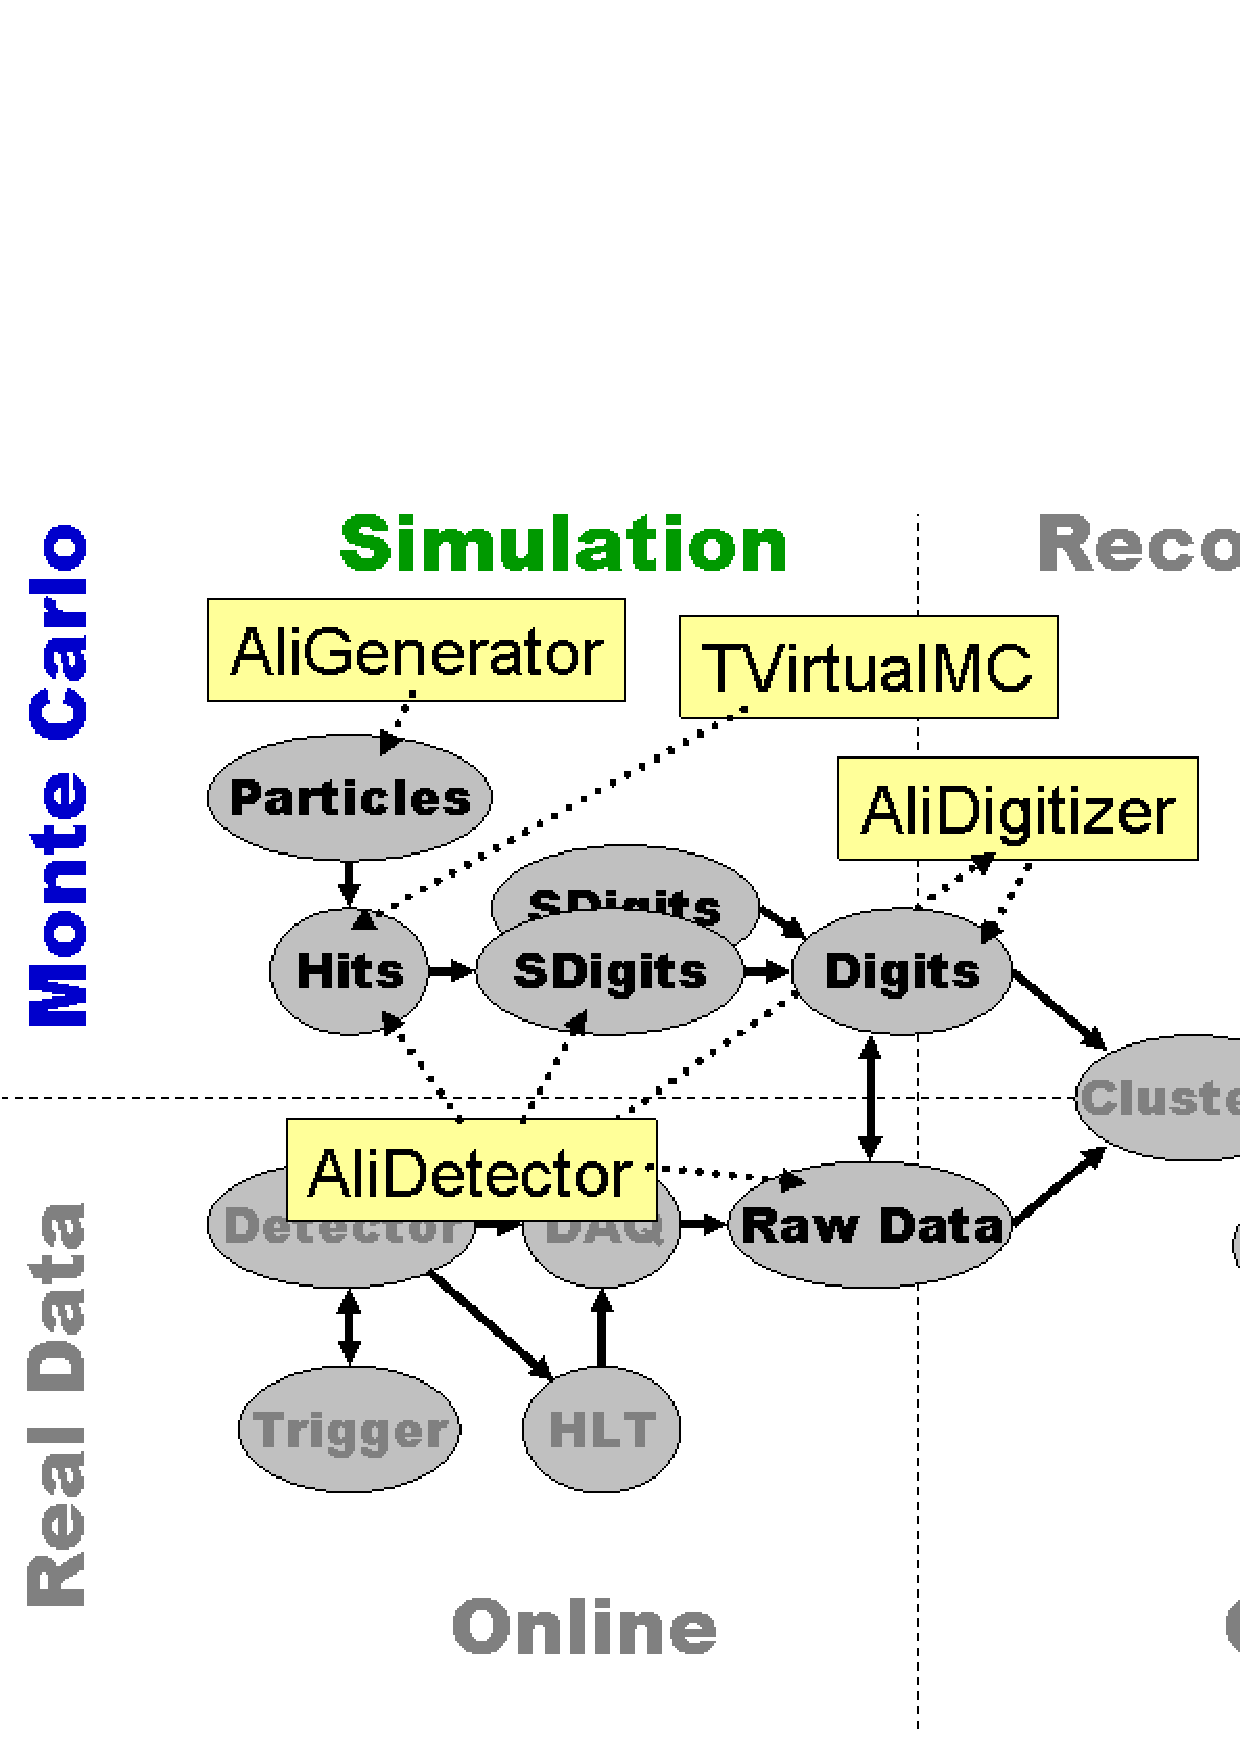
\includegraphics[width=10cm]{picts/SimulationFramework}
  \caption{Simulation framework.} \label{MC:Simulation}
\end{figure}


\noindent
\textbf{Generation of Particles}

Different generators can be used to produce particles emerging from
the collision. The class \class{IlcGenerator} is the base class
defining the virtual interface to the generator programs. The
generators are described in more detail in the ILC PPR Volume 1 and
in the next chapter.

\noindent
\textbf{Virtual Monte Carlo}

The simulation of particles traversing the detector components is
performed by a class derived from \class{TVirtualMC}. The Virtual
Monte Carlo also provides an interface to construct the geometry of
detectors. The task of the geometry description is done by the
geometrical modeler \class{TGeo}. The concrete implementation of the
virtual Monte Carlo application TVirtualMCApplication is IlcMC. The
Monte Carlos used in ILC are GEANT~3.21, GEANT~4 and FLUKA. More
information can be found on the VMC Web page:
\url{http://root.cern.ch/root/vmc}

As explained above, our strategy was to develop a virtual interface to
the detector simulation code. We call the interface to the transport
code virtual Monte Carlo. It is implemented via C++ virtual classes
and is schematically shown in Fig.~\ref{MC:vmc}. The codes that
implement the abstract classes are real C++ programs or wrapper
classes that interface to FORTRAN programs.

\begin{figure}[ht]
  \centering
  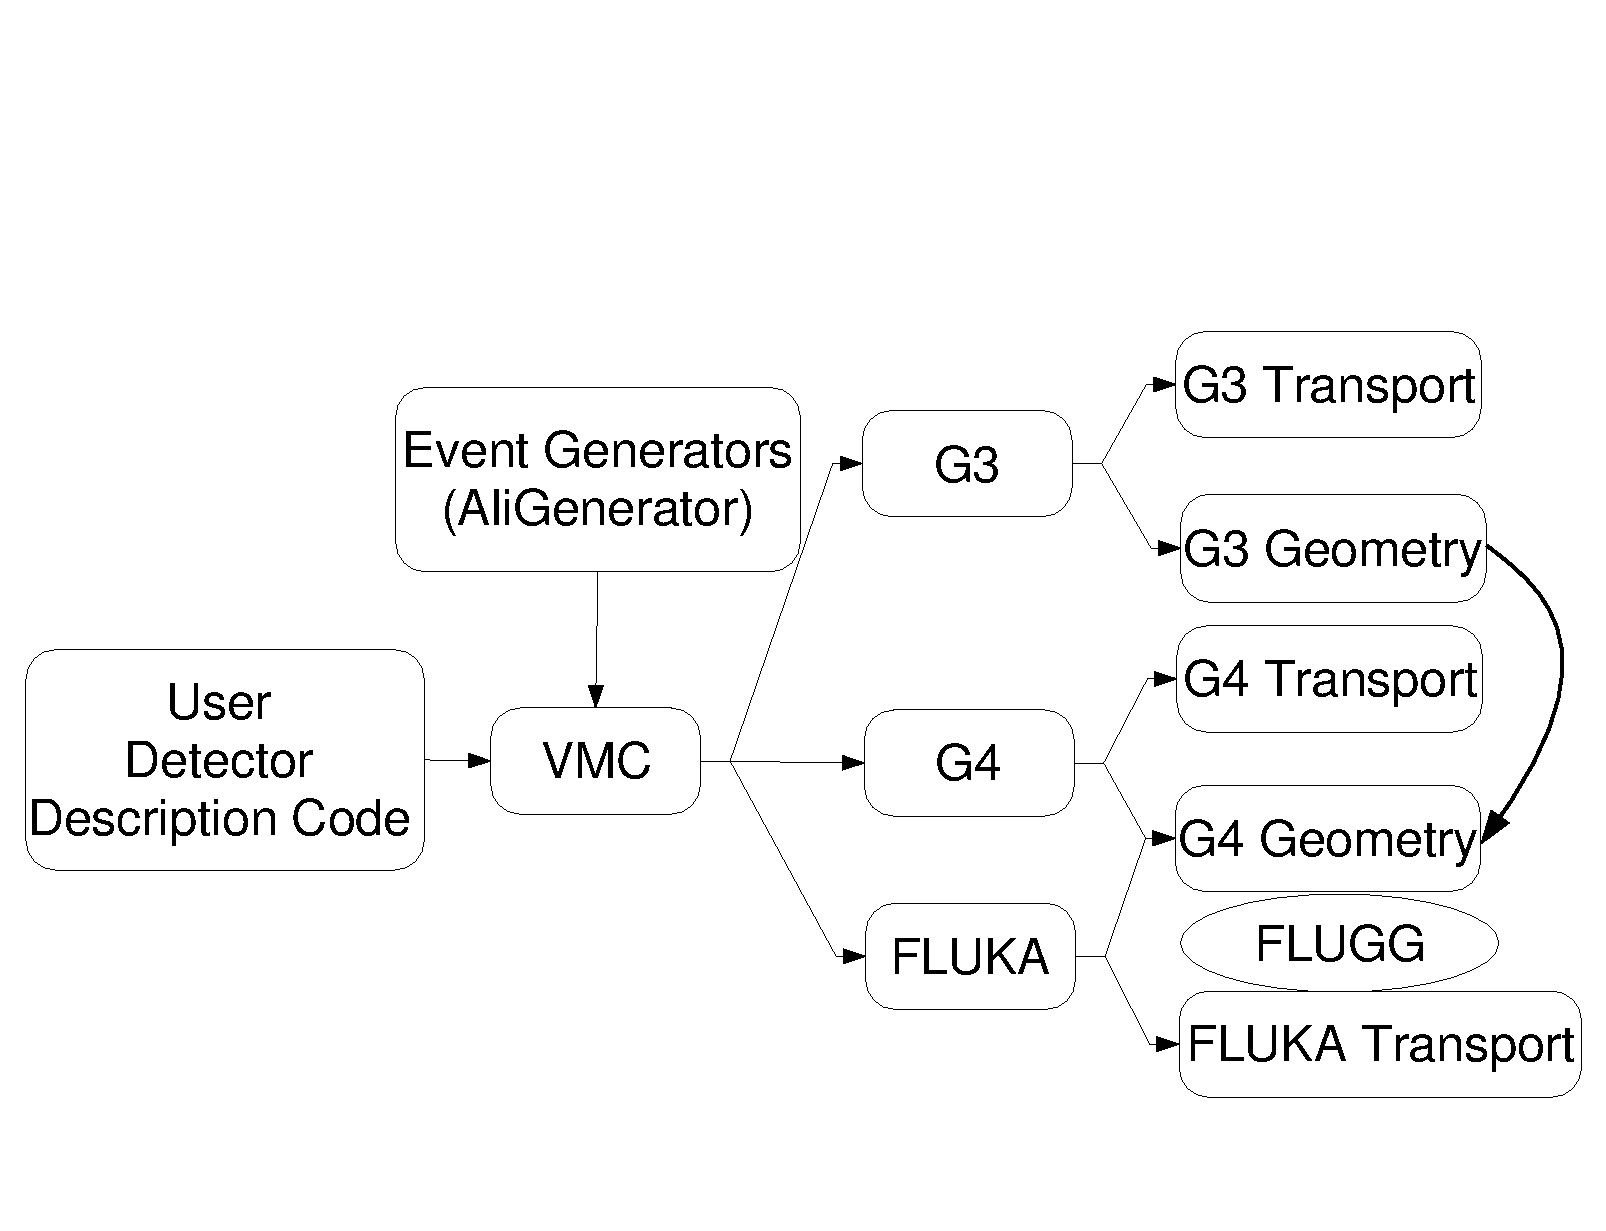
\includegraphics[width=10cm]{picts/vmc}
  \caption{Virtual \MC} \label{MC:vmc}
\end{figure}

Thanks to the virtual Monte Carlo we have converted all FORTRAN user
code developed for GEANT~3 into C++, including the geometry definition
and the user scoring routines, \texttt{StepManager}. These have been
integrated in the detector classes of the IlcRoot framework. The
output of the simulation is saved directly with ROOT I/O, simplifying
the development of the digitization and reconstruction code in C++.

\noindent
\textbf{Modules and Detectors}

Each module of the ILC detector is described by a class derived from
\class{IlcModule}. Classes for active modules (= detectors) are not
derived directly from \class{IlcModule} but from its subclass
\class{IlcDetector}. These base classes define the interface to the
simulation framework via a set of virtual methods.

\noindent
\textbf{Configuration File (Config.C)}

The configuration file is a C++ macro that is processed before the
simulation starts. It creates and configures the Monte Carlo object,
the generator object, the magnetic field map and the detector modules.
A detailed description is given below.

\noindent
\textbf{Detector Geometry}

The virtual Monte Carlo application creates and initializes the
geometry of the detector modules by calling the virtual functions
\method{CreateMaterials}, \method{CreateGeometry}, \method{Init} and
\method{BuildGeometry}.

\noindent
\textbf{Vertexes and Particles}

In case the simulated event is intended to be merged with an
underlying event, the primary vertex is taken from the file containing
the underlying event by using the vertex generator
\class{IlcVertexGenFile}. Otherwise the primary vertex is generated
according to the generator settings. Then the particles emerging from
the collision are generated and put on the stack (an instance of
\class{IlcStack}). The transport of particles through the detector is
performed by the Monte Carlo object. The decay of particles is usually
handled by the external decayer \class{IlcDecayerPythia}.

\noindent
\textbf{Hits and Track References}

The Monte Carlo simulates the transport of a particle step by step.
After each step the virtual method \method{StepManager} of the module
in which the particle currently is located is called. In this step
manager method, the hits in the detector are created by calling
\method{AddHit}. Optionally also track references (location and
momentum of simulated particles at selected places) can be created by
calling \method{AddTackReference}. \method{AddHit} has to be
implemented by each detector whereas \method{AddTackReference} is
already implemented in IlcModule. The container and the branch for the
hits -- and for the (summable) digits -- are managed by the detector
class via a set of so-called loaders. The relevant data members and
methods are fHits, fDigits, \method{ResetHits}, \method{ResetSDigits},
\method{ResetDigits},\method{MakeBranch} and \method{SetTreeAddress}.

For each detector methods like \method{PreTrack}, \method{PostTrack},
\method{FinishPrimary}, \method{FinishEvent} and \method{FinishRun}
are called during the simulation when the conditions indicated by the
method names are fulfilled.

\noindent
\textbf{Summable Digits}

Summable digits are created by calling the virtual method Hits2SDigits
of a detector. This method loops over all events, creates the summable
digits from hits and stores them in the sdigits file(s).

\noindent
\textbf{ Digitization and Merging}

Dedicated classes derived from \class{IlcDigitizer} are used for the
conversion of summable digits into digits. Since \class{IlcDigitizer}
is a \class{TTask}, this conversion is done for
the current event by the \method{Exec} method. Inside this method the summable
digits of all input streams have to be added, combined with noise,
converted to digital values taking into account possible thresholds
and stored in the digits container.

The input streams (more than one in case of merging) as well as the
output stream are managed by an object of type \method{IlcRunDigitizer}. The
methods GetNinputs, GetInputFolderName and GetOutputFolderName return
the relevant information. The run digitizer is accessible inside the
digitizer via the protected data member fManager. If the flag
fRegionOfInterest is set, only detector parts where summable digits
from the signal event are present should be digitized. When \MC labels
are assigned to digits, the stream-dependent offset given by the
method \method{GetMask} is added to the label of the summable digit.

The detector specific digitizer object is created in the virtual
method CreateDigitizer of the concrete detector class. The run
digitizer object is used to construct the detector
digitizer. The \method{Init} method of each digitizer is called before the loop
over the events starts.


A direct conversion from hits directly to digits can be implemented in
the method \method{Hits2Digits} of a detector. The loop over the events is
inside the method. Of course merging is not supported in this case.

An example of simulation script that can be used for simulation of
proton-proton collisions is provided below:

\begin{lstlisting}[language=C++, title={Simulation run}]
  void sim(Int_t nev=100) {
    IlcSimulation simulator;
    // Measure the total time spent in the simulation
    TStopwatch timer;
    timer.Start();
    // List of detectors, where both summable digits and digits are provided
    simulator.SetMakeSDigits("TRD TOF PHOS EMCAL HMPID MUON ZDC PMD FMD T0 VZERO");
    // Direct conversion of hits to digits for faster processing (ITS TPC)
    simulator.SetMakeDigitsFromHits("ITS TPC");
    simulator.Run(nev);
    timer.Stop();
    timer.Print();
  }
\end{lstlisting}

The following example shows how one can do event merging

\begin{lstlisting}[language=C++, title={Event merging}]
  void sim(Int_t nev=6) {
    IlcSimulation simulator;
    // The underlying events are stored in a separate directory.
    // Three signal events will be merged in turn with each
    // underlying event
    simulator.MergeWith("../backgr/gilc.root",3);
    simulator.Run(nev);
  }
\end{lstlisting}

\noindent
\textbf{Raw Data}

The digits stored in ROOT containers can be converted into the DATE\cite{DATE}
format that will be the `payload' of the ROOT classes containing the
raw data. This is done for the current event in the method
\method{Digits2Raw} of the detector.

The simulation of raw data is managed by the class \class{IlcSimulation}. To
create raw data DDL files it loops over all events. For each event it
creates a directory, changes to this directory and calls the method
\method{Digits2Raw} of each selected detector. In the Digits2Raw method the DDL
files of a detector are created from the digits for the current
event. 

For the conversion of the DDL files to a DATE file the
\class{IlcSimulation} class uses the tool dateStream. To create a raw
data file in ROOT format with the DATE output as payload the program ilcmdc is
utilized.

The only part that has to be implemented in each detector is
the \method{Digits2Raw} method of the detectors. In this method one file per
DDL has to be created obeying the conventions for file names and DDL
IDs. Each file is a binary file with a DDL data header in the
beginning. The DDL data header is implemented in the structure
\class{IlcRawDataHeader}. The data member fSize should be set to the total
size of the DDL raw data including the size of the header. The
attribute bit 0 should be set by calling the method \method{SetAttribute(0)} to
indicate that the data in this file is valid. The attribute bit 1 can
be set to indicate compressed raw data.

The detector-specific raw data are stored in the DDL files after the
DDL data header. The format of this raw data should be as close as
possible to the one that will be delivered by the detector. This
includes the order in which the channels will be read out.

Below we show an example of raw data creation for all the detectors

\begin{lstlisting}[language=C++]
  void sim(Int_t nev=1) {
    IlcSimulation simulator;
    // Create raw data for ALL detectors, rootify it and store in the
    // file raw,root. Do not delete the intermediate files
    simulator.SetWriteRawData("ALL","raw.root",kFALSE);
    simulator.Run(nev);
  }
\end{lstlisting}


\subsection{Configuration: example of Config.C}

The example below contains as comments the most important information:

\lstinputlisting[language=C++] {scripts/Config.C}

% -----------------------------------------------------------------------------

\subsection{Event generation}
\label{MC:Generators}
\begin{figure}[ht]
  \centering
  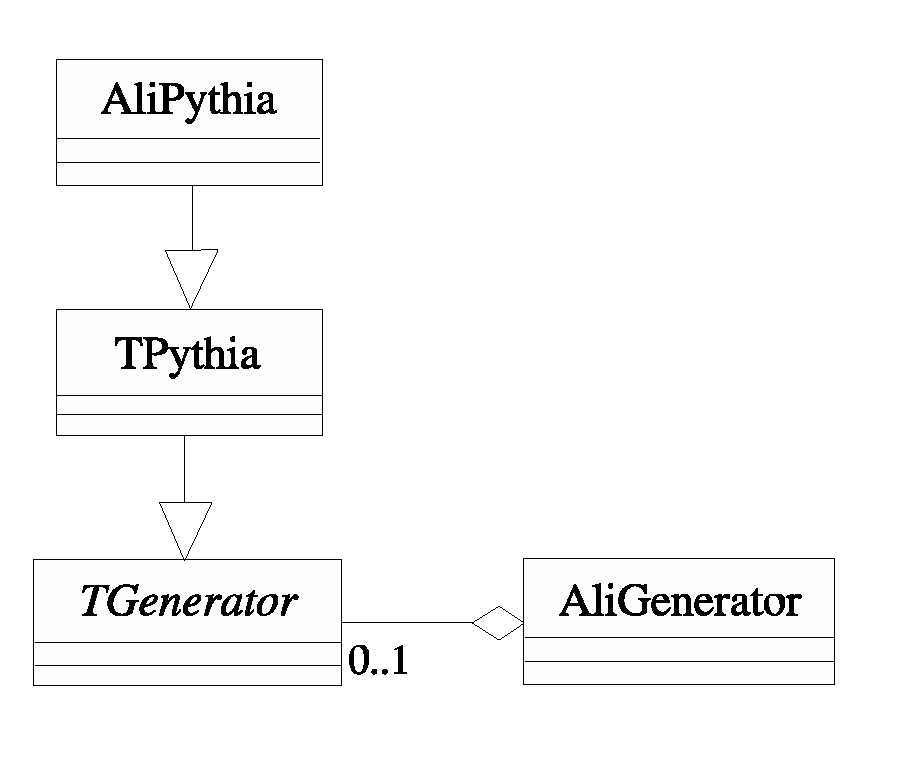
\includegraphics[width=10cm]{picts/ilcgen}
  \caption{\texttt{IlcGenerator} is the base class, which has the
    responsibility to generate the primary particles of an event. Some
    realizations of this class do not generate the particles themselves
    but delegate the task to an external generator like PYTHIA through the
    \texttt{TGenerator} interface.  }
  \label{MC:ilcgen}
\end{figure}

\subsubsection{Parameterized generation}

The event generation based on parameterization can be used to produce
signal-free final states. It avoids the dependences on a
specific model, and is efficient and flexible. It can be used to
study the track reconstruction efficiency
as a function of the initial multiplicity and occupation. 

\class{IlcGenHIJINGparam}~\cite{MC:HIJINGparam} is an example of internal
IlcRoot generator based on parameterized
pseudorapidity density and transverse momentum distributions of
charged and neutral pions and kaons. The pseudorapidity
distribution was obtained from a HIJING simulation of central
Pb--Pb collisions and scaled to a charged-particle multiplicity of
8000 in the pseudo rapidity interval $|\eta | < 0.5$. Note that
this is about 10\% higher than the corresponding value for a
rapidity density with an average ${\rm d}N/{\rm d}y$ of 8000 in
the interval $|y | < 0.5$.
The transverse-momentum distribution is parameterized from the
measured CDF pion $p_T$-distribution at $\sqrt{s} = 1.8 \, TeV$.
The corresponding kaon $p_T$-distribution was obtained from the
pion distribution by $m_T$-scaling. See Ref.~\cite{MC:HIJINGparam}
for the details of these parameterizations.

In many cases, the expected transverse momentum and rapidity
distributions of particles are known. In other cases the effect of
variations in these distributions must be investigated. In both
situations it is appropriate to use generators that produce
primary particles and their decays sampling from parameterized
spectra. To meet the different physics requirements in a modular
way, the parameterizations are stored in independent function
libraries wrapped into classes that can be plugged into the
generator. This is schematically illustrated in
Fig.~\ref{MC:evglib} where four different generator libraries can
be loaded via the abstract generator interface.

It is customary in heavy-ion event generation to superimpose
different signals on an event to tune the reconstruction
algorithms. This is possible in IlcRoot via the so-called cocktail
generator (Fig.~\ref{MC:cocktail}).  This creates events from
user-defined particle cocktails by choosing as ingredients a list
of particle generators.

\begin{figure}[ht]
  \centering
  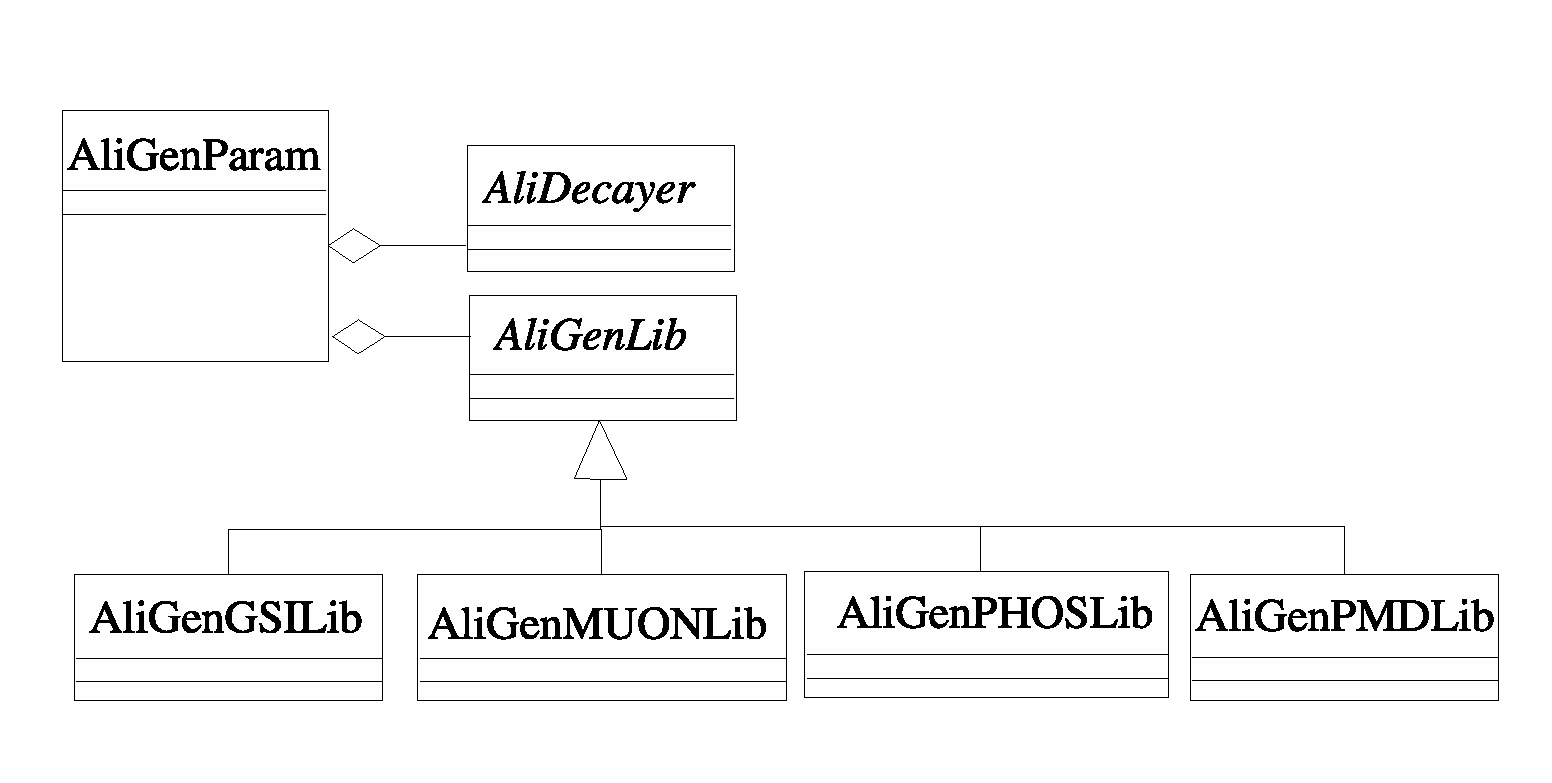
\includegraphics[width=10cm]{picts/evglib}
  \caption{\texttt{IlcGenParam} is a realization of \texttt{IlcGenerator}
    that generates particles using parameterized $\pt$ and
    pseudo-rapidity distributions. Instead of coding a fixed number of
    parameterizations directly into the class implementations, user
    defined parameterization libraries (IlcGenLib) can be connected at
    run time allowing for maximum flexibility.} \label{MC:evglib}
\end{figure}

An example of \class{IlcGenParam} usage is presented below:

\begin{lstlisting}[language=C++]
  // Example for J/psi  Production from  Parameterization 
  // using default library (IlcMUONlib)                                       
  IlcGenParam *gener = new IlcGenParam(ntracks, IlcGenMUONlib::kUpsilon);
  gener->SetMomentumRange(0,999); // Wide cut on the Upsilon momentum
  gener->SetPtRange(0,999);       // Wide cut on Pt
  gener->SetPhiRange(0. , 360.);  // Full azimutal range
  gener->SetYRange(2.5,4);        // In the acceptance of the MUON arm
  gener->SetCutOnChild(1);        // Enable cuts on Upsilon decay products
  gener->SetChildThetaRange(2,9); // Theta range for the decay products
  gener->SetOrigin(0,0,0);        // Vertex position
  gener->SetSigma(0,0,5.3);       // Sigma in (X,Y,Z) (cm) on IP position
  gener->SetForceDecay(kDiMuon);  // Upsilon->mu+ mu- decay
  gener->SetTrackingFlag(0);      // No particle transport
  gener->Init()
\end{lstlisting}

To facilitate the usage of different generators we have developed
an abstract generator interface called \texttt{IlcGenerator}, see
Fig.~\ref{MC:ilcgen}.  The objective is to provide the user with
an easy and coherent way to study a variety of physics signals as
well as full set of tools for testing and background studies. This
interface allows the study of full events, signal processes, and
a mixture of both, i.e. cocktail events (see an example later).

Several event generators are available via the abstract ROOT class
that implements the generic generator interface, \texttt{TGenerator}.
Through implementations of this abstract base class we wrap
FORTRAN \MC codes like PYTHIA, HERWIG, and HIJING that are
thus accessible from the IlcRoot classes. In particular the
interface to PYTHIA includes the use of nuclear structure
functions of LHAPDF.


\subsubsection{Pythia6}

Pythia is used for simulation of proton-proton interactions and for
generation of jets in case of event merging. An example of minimum
bias Pythia events is presented below:

\begin{lstlisting}[language=C++]
  IlcGenPythia *gener = new IlcGenPythia(-1); 
  gener->SetMomentumRange(0,999999);
  gener->SetThetaRange(0., 180.);
  gener->SetYRange(-12,12);
  gener->SetPtRange(0,1000);
  gener->SetProcess(kPyMb);        // Min. bias events
  gener->SetEnergyCMS(14000.);     // LHC energy
  gener->SetOrigin(0, 0, 0);       // Vertex position
  gener->SetSigma(0, 0, 5.3);      // Sigma in (X,Y,Z) (cm) on IP position
  gener->SetCutVertexZ(1.);        // Truncate at 1 sigma
  gener->SetVertexSmear(kPerEvent);// Smear per event
  gener->SetTrackingFlag(1);       // Particle transport
  gener->Init()
\end{lstlisting}


\subsubsection{HIJING}
HIJING (Heavy-Ion Jet Interaction Generator) combines a
QCD-inspired model of jet production~\cite{MC:HIJING} with the
Lund model~\cite{MC:LUND} for jet fragmentation.  Hard or
semi-hard parton scatterings with transverse momenta of a few GeV
are expected to dominate high-energy heavy-ion collisions.  The
HIJING model has been developed with special emphasis on the role
of mini jets in pp, pA and A--A reactions at collider energies.

Detailed systematic comparisons of HIJING results with a wide
range of data demonstrates a qualitative understanding of the
interplay between soft string dynamics and hard QCD interactions.
In particular, HIJING reproduces many inclusive spectra,
two-particle correlations, and the observed flavor and
multiplicity dependence of the average transverse momentum.

The Lund FRITIOF~\cite{MC:FRITIOF} model and the Dual Parton
Model~\cite{MC:DPM} (DPM) have guided the formulation of HIJING
for soft nucleus--nucleus reactions at intermediate energies,
$\sqrt{s_{\rm NN}}\approx 20\, GeV$.  The hadronic-collision
model has been inspired by the successful implementation of
perturbative QCD processes in PYTHIA~\cite{MC:PYTH}.  Binary
scattering with Glauber geometry for multiple interactions are
used to extrapolate to pA and A--A collisions.

Two important features of HIJING are jet quenching and nuclear
shadowing. Jet quenching is the energy loss by partons in nuclear
matter.  It is responsible for an increase of the particle
multiplicity at central rapidities.  Jet quenching is modeled by an
assumed energy loss by partons traversing dense matter.  A simple
color configuration is assumed for the multi-jet system and the Lund
fragmentation model is used for the hadronisation.  HIJING does not
simulate secondary interactions.

Shadowing describes the modification of the free nucleon parton
density in the nucleus.  At the low-momentum fractions, $x$,
observed by collisions at the LHC, shadowing results in a decrease
of the multiplicity. Parton shadowing is taken into account using
a parameterization of the modification.

Here is an example of event generation with HIJING:

\begin{lstlisting}[language=C++]
  IlcGenHijing *gener = new IlcGenHijing(-1);
  gener->SetEnergyCMS(5500.); // center of mass energy 
  gener->SetReferenceFrame("CMS"); // reference frame
  gener->SetProjectile("A", 208, 82); // projectile
  gener->SetTarget    ("A", 208, 82); // projectile
  gener->KeepFullEvent(); // HIJING will keep the full parent child chain
  gener->SetJetQuenching(1); // enable jet quenching
  gener->SetShadowing(1); // enable shadowing
  gener->SetDecaysOff(1); // neutral pion and heavy particle decays switched off
  gener->SetSpectators(0); // Don't track spectators
  gener->SetSelectAll(0); // kinematic selection
  gener->SetImpactParameterRange(0., 5.); // Impact parameter range (fm)
  gener->Init()
\end{lstlisting}

\subsubsection{Additional universal generators}

The following universal generators are available in IlcRoot:

\begin{itemize}
\item DPMJET: this is an implementation of the dual parton
  model\cite{MC:DPMJET};
\item ISAJET: a \MC event generator for pp, $\bar pp$, and $e^=e^-$
  reactions\cite{MC:ISAJET};
\item HERWIG:  \MC package for simulating Hadron Emission
  Reactions With Interfering Gluons\cite{MC:HERWIG}.
\end{itemize}

An example of HERWIG configuration in the Config.C is shown below:
\begin{lstlisting}[language=C++]
IlcGenHerwig *gener = new IlcGenHerwig(-1);
//   final state kinematic cuts
gener->SetMomentumRange(0,7000);
gener->SetPhiRange(0. ,360.);
gener->SetThetaRange(0., 180.);
gener->SetYRange(-10,10);
gener->SetPtRange(0,7000);
//   vertex position and smearing 
gener->SetOrigin(0,0,0);       // vertex position
gener->SetVertexSmear(kPerEvent);
gener->SetSigma(0,0,5.6);      // Sigma in (X,Y,Z) (cm) on IP position
//   Beam momenta
gener->SetBeamMomenta(7000,7000);
//   Beams
gener->SetProjectile("P");
gener->SetTarget("P");
//   Structure function
gener->SetStrucFunc(kGRVHO);
//   Hard scatering
gener->SetPtHardMin(200);
gener->SetPtRMS(20);
//   Min bias
gener->SetProcess(8000);
\end{lstlisting}

\subsubsection{Generators for specific studies}

\textbf{MEVSIM}

MEVSIM~\cite{MC:MEVSIM} was developed for the STAR experiment to
quickly produce a large number of A--A collisions for some
specific needs -- initially for HBT studies and for testing of
reconstruction and analysis software. However, since the user is
able to generate  specific signals, it was extended to flow and
event-by-event fluctuation analysis.  A detailed description of
MEVSIM can be found in Ref.~\cite{MC:MEVSIM}.

MEVSIM generates particle spectra according to a momentum model
chosen by the user. The main input parameters are: types and
numbers of generated particles, momentum-distribution model,
reaction-plane and azimuthal-anisotropy coefficients, multiplicity
fluctuation, number of generated events, etc. The momentum models
include factorized $p_T$ and rapidity distributions, non-expanding
and expanding thermal sources, arbitrary distributions in $y$ and
$p_T$ and others. The reaction plane and azimuthal anisotropy is
defined by the Fourier coefficients (maximum of six) including
directed and elliptical flow. Resonance production can also be
introduced.

MEVSIM was originally written in FORTRAN. It was later integrated into
IlcRoot. A complete description of the IlcRoot implementation of MEVSIM can
be found on the web page (\url{http://home.cern.ch/~radomski}).

\textbf{GeVSim}

GeVSim \cite{MC:GEVSIM} is a fast and easy-to-use \MC
event generator implemented in IlcRoot. It can provide events of
similar type configurable by the user according to the specific
needs of a simulation project, in particular, that of flow and
event-by-event fluctuation studies. It was developed to facilitate
detector performance studies and for the test of algorithms.
GeVSim can also be used to generate signal-free events to be
processed by afterburners, for example HBT processor.

GeVSim is based on the MevSim \cite{MC:MEVSIM} event generator
developed for the STAR experiment. 

GeVSim generates a list of particles by randomly sampling a
distribution function.  The parameters of single-particle spectra
and their event-by-event fluctuations are explicitly defined by
the user. Single-particle transverse-momentum and rapidity spectra
can be either selected from a menu of four predefined
distributions, the same as in MevSim, or provided by user.

Flow can be easily introduced into simulated events. The parameters of
the flow are defined separately for each particle type and can be
either set to a constant value or parameterized as a function of
transverse momentum and rapidity. Two parameterizations of elliptic
flow based on results obtained by RHIC experiments are provided.

GeVSim also has extended possibilities for simulating of
event-by-event fluctuations.  The model allows fluctuations
following an arbitrary analytically defined distribution in
addition to the Gaussian distribution provided by MevSim. It is
also possible to systematically alter a given parameter to scan
the parameter space in one run. This feature is useful when
analyzing performance with respect to, for example, multiplicity
or event-plane angle.

The current status and further development of GeVSim code and documentation
can be found in Ref.~\cite{MC:Radomski}.

\textbf{HBT processor}

Correlation functions constructed with the data produced by MEVSIM
or any other event generator are normally flat in the region of
small relative momenta.  The HBT-processor afterburner introduces
two particle correlations into the set of generated particles.  It
shifts the momentum of each particle so that the correlation
function of a selected model is reproduced.  The imposed
correlation effects due to Quantum Statistics (QS) and Coulomb
Final State Interactions (FSI) do not affect the single-particle
distributions and multiplicities. The event structures before and
after passing through the HBT processor are identical.  Thus, the
event reconstruction procedure with and without correlations is
also identical. However, the track reconstruction efficiency, momentum
resolution and particle identification need not to be, since
correlated particles have a special topology at small relative
velocities. We can thus verify the influence of various
experimental factors on the correlation functions.

The method, proposed by L.~Ray and G.W.~Hoffmann \cite{MC:HBTproc}
is based on random shifts of the particle three-momentum within a
confined range.  After each shift, a comparison is made with
correlation functions resulting from the assumed model of the
space--time distribution and with the single-particle spectra
which should remain unchanged.  The shift is kept if the
$\chi^2$-test shows better agreement.  The process is iterated
until satisfactory agreement is achieved.  In order to construct
the correlation function, a reference sample is made by mixing
particles from some consecutive events.  Such a method has an
important impact on the simulations when at least two events must
be processed simultaneously.

Some specific features of this approach are important for practical
use:
\begin{itemize}
\item{} the HBT processor can simultaneously generate correlations of up
  to two particle types (e.g. positive and negative pions).
  Correlations of other particles can be added subsequently.
\item{} the form of the correlation function has to be parameterized
  analytically.  One and three dimensional parameterizations are
  possible.
\item{} a static source is usually assumed. Dynamical effects,
  related to
  expansion or flow, can be simulated in a stepwise form by repeating
  simulations for different values of the space--time parameters
  associated with different kinematic intervals.
\item{} Coulomb effects may be introduced by one of three
  approaches: Gamow
  factor, experimentally modified Gamow correction and integrated
  Coulomb wave functions for discrete values of the source radii.
\item{} Strong interactions are not implemented.
\end{itemize}

The detailed description of the HBT processor can be found
elsewhere~\cite{MC:PiotrSk}.

\textbf{Flow afterburner}

Azimuthal anisotropies, especially elliptic flow, carry unique
information about collective phenomena and consequently are
important for the study of heavy-ion collisions.  Additional
information can be obtained studying different heavy-ion
observables, especially jets, relative to the event plane.
Therefore it is necessary to evaluate the capability of ILC to
reconstruct the event plane and study elliptic flow.

Since there is not a well understood microscopic description of
the flow effect it cannot be correctly simulated by microscopic
event generators.  Therefore, to generate events with flow the user has
to use event generators based on macroscopic models, like GeVSim
\cite{MC:GEVSIM} or an afterburner which can generate flow on top
of events generated by event generators based on the microscopic
description of the interaction.  In the IlcRoot framework such a
flow afterburner is implemented.

The algorithm to apply azimuthal correlation consists in shifting the
azimuthal coordinates of the particles.  The transformation is given
by \cite{MC:POSCANCER}:


\[
\varphi \rightarrow \varphi '=\varphi +\Delta \varphi \]
\[
\Delta \varphi =\sum _{n}\frac{-2}{n}v_{n}\left( p_{t},y\right)
\sin  n \times \left( \varphi -\psi \right) \] where \(
v_{n}(p_{t},y) \) is the flow coefficient to be obtained, \( n \)
is the harmonic number and \( \psi \) is the event-plane angle.
Note that the algorithm is deterministic and does not contain any
random numbers generation.

The value of the flow coefficient can be either constant or parameterized as a
function of transverse momentum and rapidity.  Two parameterizations
of elliptic flow are provided as in GeVSim.

\begin{lstlisting}[language=C++]
  IlcGenGeVSim* gener = new IlcGenGeVSim(0);

  mult = 2000; // Mult is the number of charged particles in |eta| < 0.5
  vn = 0.01;   // Vn

  Float_t sigma_eta  = 2.75; // Sigma of the Gaussian dN/dEta
  Float_t etamax     = 7.00; // Maximum eta

  // Scale from multiplicity in |eta| < 0.5 to |eta| < |etamax|	
  Float_t mm = mult * (TMath::Erf(etamax/sigma_eta/sqrt(2.)) /
  TMath::Erf(0.5/sigma_eta/sqrt(2.))); 

  // Scale from charged to total multiplicity
  mm *= 1.587;

  // Define particles

  // 78% Pions (26% pi+, 26% pi-, 26% p0)              T = 250 MeV
  IlcGeVSimParticle *pp =  
  new IlcGeVSimParticle(kPiPlus,  1, 0.26 * mm, 0.25, sigma_eta) ;
  IlcGeVSimParticle *pm =  
  new IlcGeVSimParticle(kPiMinus, 1, 0.26 * mm, 0.25, sigma_eta) ;
  IlcGeVSimParticle *p0 =  
  new IlcGeVSimParticle(kPi0,     1, 0.26 * mm, 0.25, sigma_eta) ;

  // 12% Kaons (3% K0short, 3% K0long, 3% K+, 3% K-)   T = 300 MeV
  IlcGeVSimParticle *ks =  
  new IlcGeVSimParticle(kK0Short, 1, 0.03 * mm, 0.30, sigma_eta) ;
  IlcGeVSimParticle *kl =
  new IlcGeVSimParticle(kK0Long,  1, 0.03 * mm, 0.30, sigma_eta) ;
  IlcGeVSimParticle *kp =
  new IlcGeVSimParticle(kKPlus,   1, 0.03 * mm, 0.30, sigma_eta) ;
  IlcGeVSimParticle *km =
  new IlcGeVSimParticle(kKMinus,  1, 0.03 * mm, 0.30, sigma_eta) ;

  // 10% Protons / Neutrons (5% Protons, 5% Neutrons)  T = 250 MeV
  IlcGeVSimParticle *pr =
  new IlcGeVSimParticle(kProton,  1, 0.05 * mm, 0.25, sigma_eta) ;
  IlcGeVSimParticle *ne =
  new IlcGeVSimParticle(kNeutron, 1, 0.05 * mm, 0.25, sigma_eta) ;

  // Set Elliptic Flow properties 	

  Float_t pTsaturation = 2. ;

  pp->SetEllipticParam(vn,pTsaturation,0.) ;
  pm->SetEllipticParam(vn,pTsaturation,0.) ;
  p0->SetEllipticParam(vn,pTsaturation,0.) ;
  pr->SetEllipticParam(vn,pTsaturation,0.) ;
  ne->SetEllipticParam(vn,pTsaturation,0.) ;
  ks->SetEllipticParam(vn,pTsaturation,0.) ;
  kl->SetEllipticParam(vn,pTsaturation,0.) ;
  kp->SetEllipticParam(vn,pTsaturation,0.) ;
  km->SetEllipticParam(vn,pTsaturation,0.) ;

  // Set Direct Flow properties	

  pp->SetDirectedParam(vn,1.0,0.) ;
  pm->SetDirectedParam(vn,1.0,0.) ;
  p0->SetDirectedParam(vn,1.0,0.) ;
  pr->SetDirectedParam(vn,1.0,0.) ;
  ne->SetDirectedParam(vn,1.0,0.) ;
  ks->SetDirectedParam(vn,1.0,0.) ;
  kl->SetDirectedParam(vn,1.0,0.) ;
  kp->SetDirectedParam(vn,1.0,0.) ;
  km->SetDirectedParam(vn,1.0,0.) ;

  // Add particles to the list

  gener->AddParticleType(pp) ;
  gener->AddParticleType(pm) ;
  gener->AddParticleType(p0) ;
  gener->AddParticleType(pr) ;
  gener->AddParticleType(ne) ;
  gener->AddParticleType(ks) ;
  gener->AddParticleType(kl) ;
  gener->AddParticleType(kp) ;
  gener->AddParticleType(km) ;

  // Random Ev.Plane

  TF1 *rpa = new TF1("gevsimPsiRndm","1", 0, 360);

  gener->SetPtRange(0., 9.) ; // Used for bin size in numerical integration
  gener->SetPhiRange(0, 360);

  gener->SetOrigin(0, 0, 0);    // vertex position
  gener->SetSigma(0, 0, 5.3);   // Sigma in (X,Y,Z) (cm) on IP position
  gener->SetCutVertexZ(1.);     // Truncate at 1 sigma
  gener->SetVertexSmear(kPerEvent); 
  gener->SetTrackingFlag(1);
  gener->Init()
\end{lstlisting}

\textbf{Generator for e$^+$e$^-$ pairs in Pb--Pb collisions}

In addition to strong interactions of heavy ions in central and
peripheral collisions, ultra-peripheral collisions of ions give
rise to coherent, mainly electromagnetic, interactions among which
the dominant process is is the (multiple) e$^+$e$^-$-pair
production \cite{MC:AlscherHT97}
\begin{equation}
  AA \to AA + n({\rm e}^+{\rm e}^-), \label{nee}
\end{equation}
where $n$ is the pair multiplicity. Most electron--positron pairs
are produced into the very forward direction escaping the
experiment. However, for  Pb--Pb collisions at the LHC the
cross-section of this process, about 230 \, ${\rm kb}$, is
enormous. A sizable fraction of pairs produced with large-momentum
transfer can contribute to the hit rate in the forward detectors
increasing the occupancy or trigger rate. In order to study this
effect an event generator for   e$^+$e$^-$-pair production has
been implemented in the IlcRoot framework \cite{MC:Sadovsky}. The
class \texttt{TEpEmGen} is a realisation of the \texttt{TGenerator}
interface for external generators and wraps the FORTRAN code used
to calculate the differential cross-section. \texttt{IlcGenEpEmv1}
derives from \texttt{IlcGenerator} and uses the external generator to
put the pairs on the IlcRoot particle stack.


\subsubsection{Combination of generators: IlcGenCocktail}

\begin{figure}[ht]
  \centering
  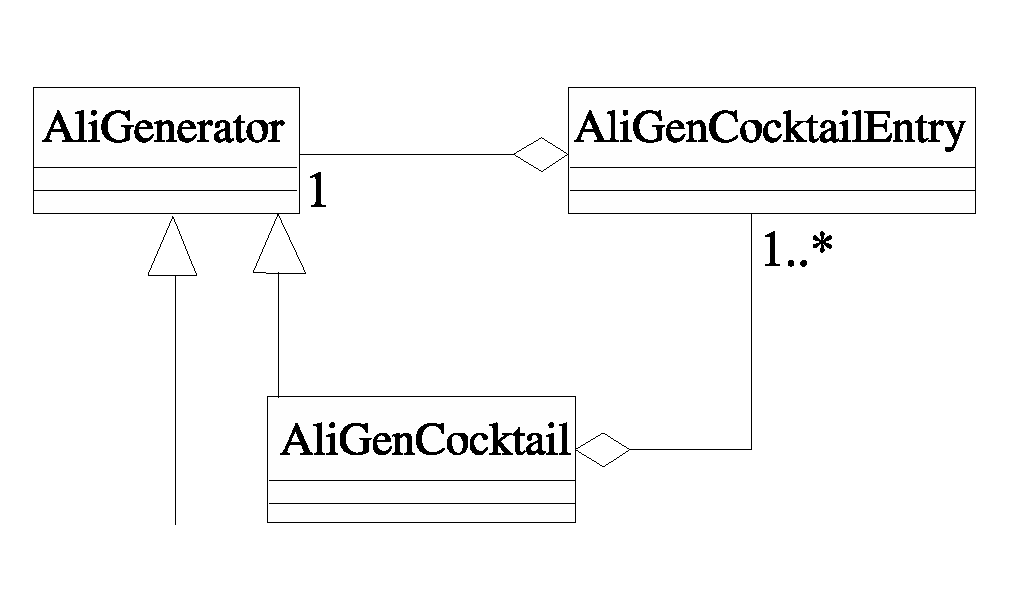
\includegraphics[width=10cm]{picts/cocktail}
  \caption{The \texttt{IlcGenCocktail} generator is a realization of {\tt
      IlcGenerator} which does not generate particles itself but
    delegates this task to a list of objects of type {\tt
      IlcGenerator} that can be connected as entries ({\tt
      IlcGenCocktailEntry}) at run time. In this way different physics
    channels can be combined in one event.} \label{MC:cocktail}
\end{figure}

Here is an example of cocktail, used for studies in the TRD detector:

\begin{lstlisting}[language=C++]
  // The cocktail generator
  IlcGenCocktail *gener  = new IlcGenCocktail();
  
  // Phi meson (10 particles)
  IlcGenParam *phi = 
  new IlcGenParam(10,new IlcGenMUONlib(),IlcGenMUONlib::kPhi,"Vogt PbPb");
  phi->SetPtRange(0, 100);
  phi->SetYRange(-1., +1.);
  phi->SetForceDecay(kDiElectron);

  // Omega meson (10 particles)
  IlcGenParam *omega = 
  new IlcGenParam(10,new IlcGenMUONlib(),IlcGenMUONlib::kOmega,"Vogt PbPb");
  omega->SetPtRange(0, 100);
  omega->SetYRange(-1., +1.);
  omega->SetForceDecay(kDiElectron);
  
  // J/psi 
  IlcGenParam *jpsi = new IlcGenParam(10,new IlcGenMUONlib(),
  IlcGenMUONlib::kJpsiFamily,"Vogt PbPb");
  jpsi->SetPtRange(0, 100);
  jpsi->SetYRange(-1., +1.);
  jpsi->SetForceDecay(kDiElectron);

  // Upsilon family
  IlcGenParam *ups = new IlcGenParam(10,new IlcGenMUONlib(),
  IlcGenMUONlib::kUpsilonFamily,"Vogt PbPb");
  ups->SetPtRange(0, 100);
  ups->SetYRange(-1., +1.);
  ups->SetForceDecay(kDiElectron);
  
  // Open charm particles
  IlcGenParam *charm = new IlcGenParam(10,new IlcGenMUONlib(), 
  IlcGenMUONlib::kCharm,"central");
  charm->SetPtRange(0, 100);
  charm->SetYRange(-1.5, +1.5);
  charm->SetForceDecay(kSemiElectronic);

  // Beauty particles: semi-electronic decays
  IlcGenParam *beauty = new IlcGenParam(10,new IlcGenMUONlib(), 
  IlcGenMUONlib::kBeauty,"central");
  beauty->SetPtRange(0, 100);
  beauty->SetYRange(-1.5, +1.5);
  beauty->SetForceDecay(kSemiElectronic);

  // Beauty particles to J/psi ee
  IlcGenParam *beautyJ = new IlcGenParam(10, new IlcGenMUONlib(), 
  IlcGenMUONlib::kBeauty,"central");
  beautyJ->SetPtRange(0, 100);
  beautyJ->SetYRange(-1.5, +1.5);
  beautyJ->SetForceDecay(kBJpsiDiElectron);

  // Adding all the components of the cocktail
  gener->AddGenerator(phi,"Phi",1);
  gener->AddGenerator(omega,"Omega",1);
  gener->AddGenerator(jpsi,"J/psi",1);
  gener->AddGenerator(ups,"Upsilon",1);
  gener->AddGenerator(charm,"Charm",1);
  gener->AddGenerator(beauty,"Beauty",1);
  gener->AddGenerator(beautyJ,"J/Psi from Beauty",1);

  // Settings, common for all components
  gener->SetOrigin(0, 0, 0);    // vertex position
  gener->SetSigma(0, 0, 5.3);   // Sigma in (X,Y,Z) (cm) on IP position
  gener->SetCutVertexZ(1.);     // Truncate at 1 sigma
  gener->SetVertexSmear(kPerEvent); 
  gener->SetTrackingFlag(1);
  gener->Init();
\end{lstlisting}


\subsection{Particle transport}

\subsubsection{TGeo essential information}

A detailed description of the Root geometry package is available in
the Root User's Guide\cite{RootUsersGuide}. Several examples can be
found in \$ROOTSYS/tutorials, among them assembly.C, csgdemo.C,
geodemo.C, nucleus.C, rootgeom.C, etc. Here we show a simple usage for
export/import of the ILC geometry and for check for overlaps and
extrusions:

\begin{lstlisting}[language=C++]
  ilcroot
  root [0] gIlc->Init()
  root [1] gGeoManager->Export("geometry.root")
  root [2] .q
  ilcroot
  root [0] TGeoManager::Import("geometry.root")
  root [1] gGeoManager->CheckOverlaps()
  root [2] gGeoManager->PrintOverlaps()
  root [3] new TBrowser
  # Now you can navigate in Geometry->Illegal overlaps
  # and draw each overlap (double click on it)
\end{lstlisting}

\subsubsection{Visualization}

Below we show an example of VZERO visualization using the Root
geometry package:

\begin{lstlisting}[language=C++]
  ilcroot
  root [0] gIlc->Init()
  root [1] TGeoVolume *top = gGeoManager->GetMasterVolume()
  root [2] Int_t nd = top->GetNdaughters()
  root [3] for (Int_t i=0; i<nd; i++) \
  top->GetNode(i)->GetVolume()->InvisibleAll()
  root [4] TGeoVolume *v0ri = gGeoManager->GetVolume("V0RI")
  root [5] TGeoVolume *v0le = gGeoManager->GetVolume("V0LE")
  root [6] v0ri->SetVisibility(kTRUE);
  root [7] v0ri->VisibleDaughters(kTRUE);
  root [8] v0le->SetVisibility(kTRUE);
  root [9] v0le->VisibleDaughters(kTRUE);
  root [10] top->Draw();

\end{lstlisting}

\subsubsection{Particle decays}

We use Pythia to carry one particle decays during the transport. The
default decay channels can be seen in the following way:

\begin{lstlisting}[language=C++]
  ilcroot
  root [0] IlcPythia * py = IlcPythia::Instance()
  root [1] py->Pylist(12); >> decay.list
\end{lstlisting}

The file decay.list will contain the list of particles decays
available in Pythia. Now if we want to force the decay $\Lambda^0 \to
p \pi^-$, the following lines should be included in the Config.C
before we register the decayer:

\begin{lstlisting}[language=C++]
  IlcPythia * py = IlcPythia::Instance();
  py->SetMDME(1059,1,0);
  py->SetMDME(1060,1,0);
  py->SetMDME(1061,1,0);
\end{lstlisting}

where 1059,1060 and 1061 are the indexes of the decay channel (from
decay.list above) we want to switch off.

\subsubsection{Examples}

\noindent
\textbf{Fast simulation}

This example is taken from the macro
\$ILC\_ROOT/FASTSIM/fastGen.C. It shows how one can create a
Kinematics tree which later can be used as input for the particle
transport. A simple selection of events with high multiplicity is
implemented. 

\lstinputlisting[language=C++] {scripts/fastGen.C}
\noindent
\textbf{Reading of kinematics tree as input for the particle transport}

We suppose that the macro fastGen.C above has been used to generate
the corresponding sent of files: gilc.root and Kinematics.root, and
that they are stored in a separate subdirectory, for example kine. Then
the following code in Config.C will read the set of files and put them
in the stack for transport:

\begin{lstlisting}[language=C++]
  IlcGenExtFile *gener = new IlcGenExtFile(-1);

  gener->SetMomentumRange(0,14000);
  gener->SetPhiRange(0.,360.);
  gener->SetThetaRange(45,135);
  gener->SetYRange(-10,10);
  gener->SetOrigin(0, 0, 0);  //vertex position
  gener->SetSigma(0, 0, 5.3);   //Sigma in (X,Y,Z) (cm) on IP position

  IlcGenReaderTreeK * reader = new IlcGenReaderTreeK();
  reader->SetFileName("../gilc.root");

  gener->SetReader(reader);
  gener->SetTrackingFlag(1);
  
  gener->Init();
\end{lstlisting}

\noindent
\textbf{Usage of different generators}

A lot of examples are available in
\$ILC\_ROOT/macros/Config\_gener.C. The correspondent part can be
extracted and placed in the relevant Config.C file.


%%%%%%%%%%%%%%%%%%%%%%%%%%%%%%%%%%%%%%%%%%%%%%%%%%%%%%%%%%%%%%%%%%%%%%%%%%%%%%%


\newpage 
%\cleardoublepage 
\section{Reconstruction}

% -----------------------------------------------------------------------------

\subsection{Reconstruction Framework}

This chapter
focuses on the reconstruction framework from the (detector) software
developers point of view. 

Wherever it is not specified explicitly as different,  we refer 
to the `global ILC coordinate system'\cite{CoordinateSystem}. It is a right-handed coordinate
system with
the $z$ axis coinciding with the beam-pipe axis and going in the direction 
opposite to the muon arm, the $y$ axis going up, and the origin of
coordinates defined by the intersection point of the $z$ axis 
and the central-membrane plane of TPC.

Here is a reminder of the following terms which are used in the
description of the reconstruction framework (see also section \ref{IlcRootFramework}):
\begin{itemize}
\item {\it Digit}: This is a digitized signal (ADC count) obtained by 
  a sensitive pad of a detector at a certain time.
\item {\it Cluster}: This is a set of adjacent (in space and/or in time)
  digits that were presumably generated by the same particle crossing the 
  sensitive element of a detector.
\item Reconstructed {\it space point}: This is the estimation of the
  position where a particle crossed the sensitive element of a detector
  (often, this is done by calculating the center of gravity of the
  `cluster').
\item Reconstructed {\it track}: This is a set of five parameters (such as the
  curvature and the angles with respect to the coordinate axes) of the particle's
  trajectory together with the corresponding covariance matrix estimated at a given
  point in space.

\end{itemize}

The input to the reconstruction framework are digits in root tree
format or raw data format. First a local reconstruction of clusters is
performed in each detector. Then vertexes and tracks are reconstructed
and the particle identification is carried on. The output of the reconstruction
is the Event Summary Data (ESD). The \class{IlcReconstruction} class provides
a simple user interface to the reconstruction framework which is
explained in the source code and. 

\begin{figure}[ht]
  \centering
  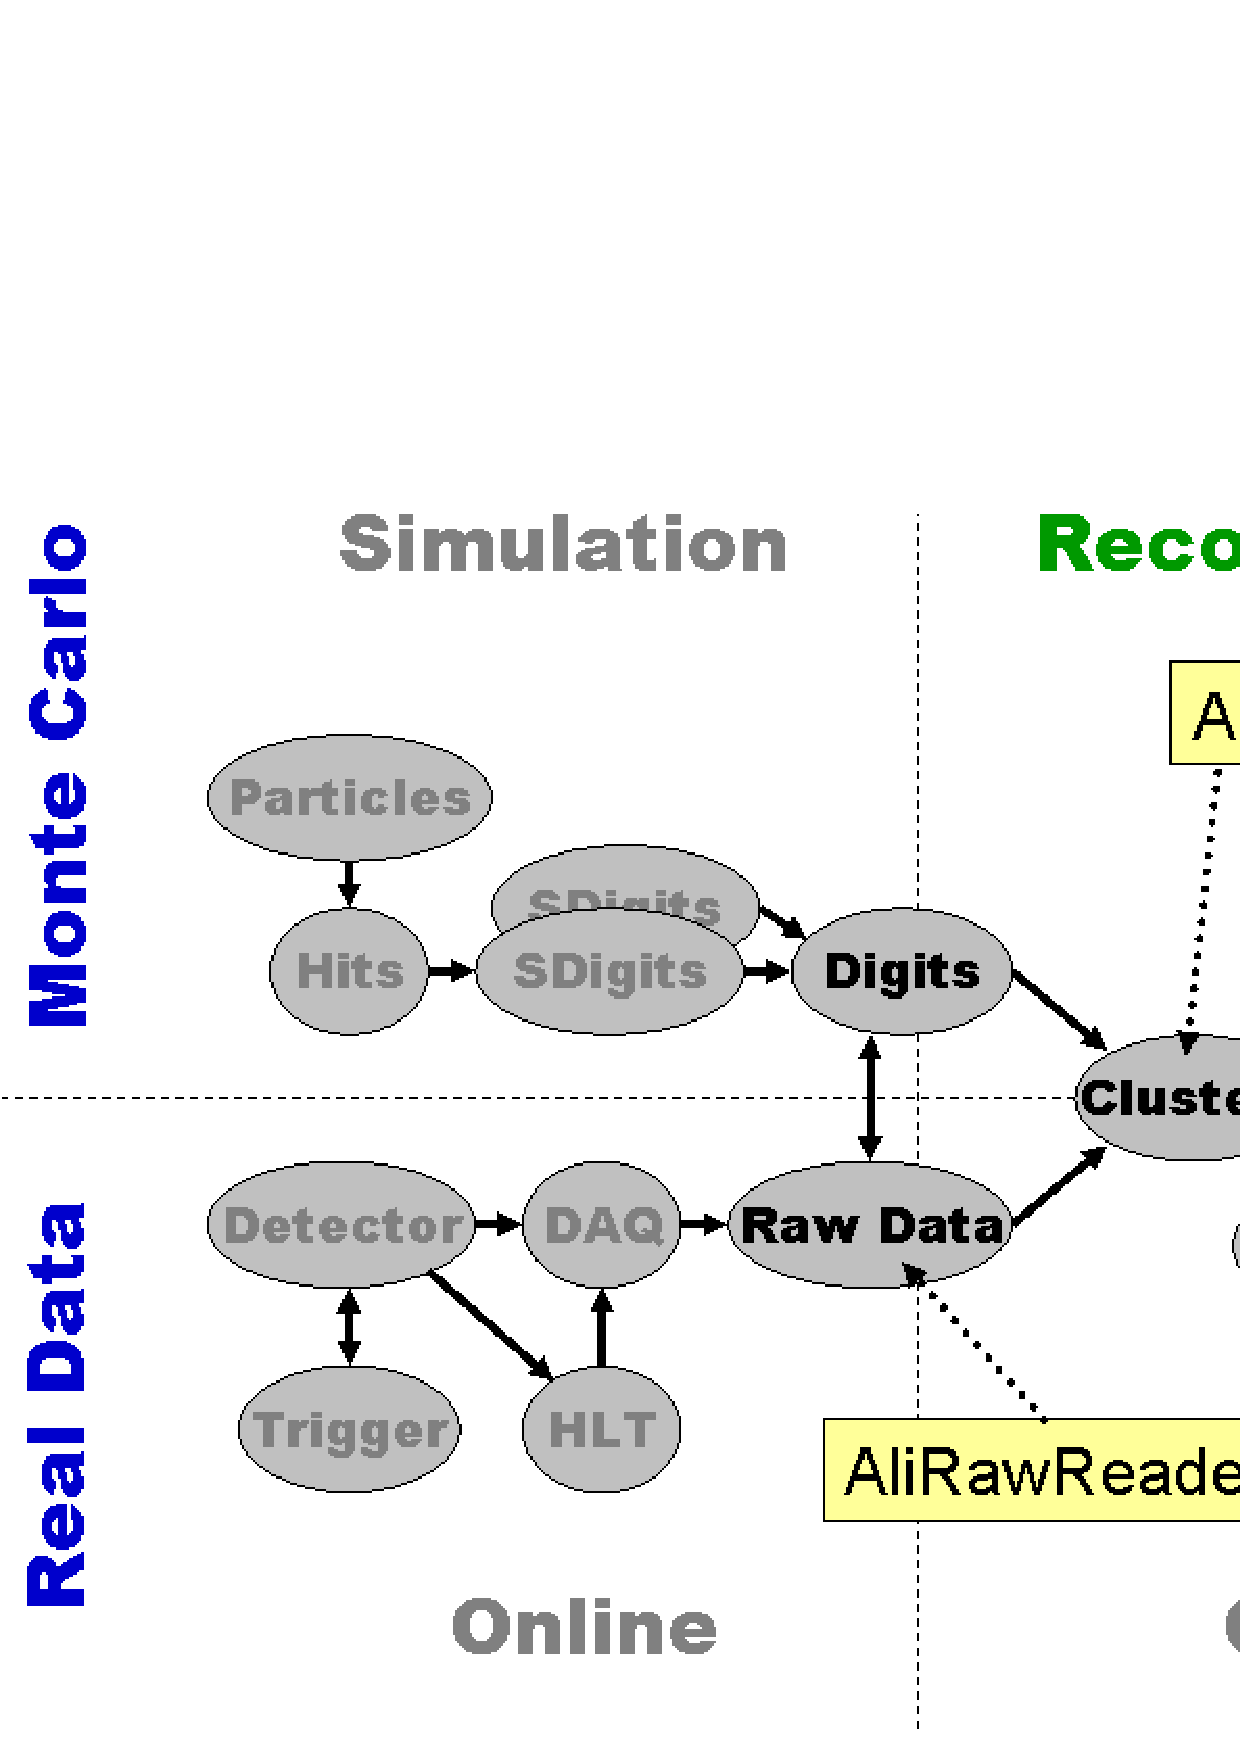
\includegraphics[width=10cm]{picts/ReconstructionFramework}
  \caption{Reconstruction framework.} \label{MC:Reconstruction}
\end{figure}

\textbf{Requirements and Guidelines}

The development of the reconstruction framework has been carried on
according to the following requirements and guidelines:
\begin{itemize}
\item the prime goal of the reconstruction is to provide the data that
  is needed for a  physics analysis; 
\item the reconstruction should be aimed for high efficiency, purity and resolution.
\item the user should have an easy to use interface to extract the
  required information from the ESD; 
\item the reconstruction code should be efficient but also maintainable;
\item the reconstruction should be as flexible as possible.
  It should be possible to do the reconstruction in one detector even in
  the case that other detectors are not operational. 
  To achieve such a flexibility each detector module should be able to
  \begin{itemize}
  \item find tracks starting from seeds provided by another detector
    (external seeding), 
  \item find tracks without using information from other detectors
    (internal seeding), 
  \item find tracks from external seeds and add tracks from internal seeds
  \item and propagate tracks through the detector using the already
    assigned clusters in inward and outward direction. 
  \end{itemize}
\item where it is appropriate, common (base) classes should be used in
  the different reconstruction modules;
\item the interdependencies between the reconstruction modules should
  be minimized. 
  If possible the exchange of information between detectors should be
  done via a common track class. 
\item the chain of reconstruction program(s) should be callable and
  steerable in an easy way;
\item there should be no assumptions on the structure or names of files
  or on the number or order of events;
\item each class, data member and method should have a correct,
  precise and helpful html documentation. 
\end{itemize}


\noindent
\textbf{IlcReconstructor}

The interface from the steering class \class{IlcReconstruction} to the
detector specific reconstruction code is defined by the base class
\class{IlcReconstructor}. For each detector there is a derived reconstructor
class. The user can set options for each reconstructor in format of a
string parameter which is accessible inside the reconstructor via the
method GetOption. 

The detector specific reconstructors are created via
plugins. Therefore they must have a default constructor. If no plugin
handler is defined by the user (in .rootrc), it is assumed that the
name of the reconstructor for detector DET is IlcDETReconstructor and
that it is located in the library libDETrec.so (or libDET.so).

\noindent
\textbf{Input Data}

If the input data is provided in format of root trees, either the
loaders or directly the trees are used to access the digits. In case
of raw data input the digits are accessed via a raw reader. 

If a gilc.root file exists, the run loader will be retrieved from
it. Otherwise the run loader and the headers will be created from the
raw data. The reconstruction can not work if there is no gilc.root file
and no raw data input.

\noindent
\textbf{Output Data}

The clusters (rec. points) are considered as intermediate output and
are stored in root trees handled by the loaders. The final output of
the reconstruction is a tree with objects of type \class{IlcESD} stored in the
file IlcESDs.root. This Event Summary Data (ESD) contains lists of
reconstructed tracks/particles and global event properties. The detailed
description of the ESD can be found in section \ref{ESD}.

\noindent
\textbf{Local Reconstruction (Clusterization)}

The first step of the reconstruction is the so called ``local
reconstruction''. It is executed for each detector separately and
without exchanging information with other detectors. Usually the
clusterization is done in this step. 

The local reconstruction is invoked via the method \method{Reconstruct} of the
reconstructor object. Each detector reconstructor runs the local
reconstruction for all events. The local reconstruction method is
only called if the method HasLocalReconstruction of the reconstructor
returns kTRUE. 

Instead of running the local reconstruction directly on raw data, it
is possible to first convert the raw data digits into a digits tree
and then to call the \method{Reconstruct} method with a tree as input
parameter. This conversion is done by the method ConvertDigits. The
reconstructor has to announce that it can convert the raw data digits
by returning kTRUE in the method \method{HasDigitConversion}.

\noindent
\textbf{Vertexing}

The current reconstruction of the primary-vertex 
position in ILC is done using the information provided by the 
silicon pixel detectors, which constitute the two innermost layers of the 
ITS.

The algorithm starts with looking at the
distribution of the $z$ coordinates of the reconstructed space points 
in the first pixel layers.
At a vertex $z$ coordinate $z_{\rm true} = 0$ the distribution is 
symmetric and 
its centroid ($z_{\rm cen}$) is very close to the nominal
vertex position. When the primary vertex is moved along the $z$ axis, an 
increasing fraction
of hits will be lost and the centroid of the distribution no longer gives
the primary
vertex position. However, for primary vertex locations not too far from 
$z_{\rm true} = 0$ 
(up to about 12~cm), the centroid of the distribution is still correlated to 
the true vertex position.
The saturation effect at large $z_{\rm true}$ values of the vertex position 
($z_{\rm true} = $12--15~cm) 
is, however, not critical, since this procedure is only meant to find a rough 
vertex position, in order to introduce some cut along $z$.

To find the final vertex position,
the correlation between the points $z_1$, $z_2$ in the two layers
was considered. More details and performance studies are available in
\cite{PPRVII}.

The primary vertex is reconstructed by a vertexer object derived from
\class{IlcVertexer}. After the local reconstruction was done for all detectors
the vertexer method \method{FindVertexForCurrentEvent} is called for each
event. It returns a pointer to a vertex object of type \class{IlcESDVertex}.

The vertexer object is created by the method \method{CreateVertexer} of the
reconstructor. So far only the ITS is used to determine the primary
vertex (\class{IlcITSVertexerZ} class).

The precision of the primary vertex reconstruction in the bending plane 
required for the reconstruction of D and B mesons in pp events
can be achieved only after the tracking is done. The method is
implemented in \class{IlcITSVertexerTracks}. It is called as a second
estimation of the primary vertex. The details of the algorithm can be
found in Appendix \ref{VertexerTracks}.

\noindent
\textbf{Combined Track Reconstruction}
The combined track reconstruction tries to accumulate the information from
different detectors in order to optimize the track reconstruction performance. 
The result of this is stored in the combined track objects.
The \class{IlcESDTrack} class also
provides the possibility to exchange information between detectors
without introducing dependencies between the reconstruction modules. 
This is achieved by using just integer indexes pointing to the
specific track objects, which on the other hand makes it possible to
retrieve the full information if needed. 
The list of combined tracks can be kept in memory and passed from one
reconstruction module to another. 
The storage of the combined tracks should be done in the standard way.

The classes responsible for the reconstruction of tracks are derived
from \class{IlcTracker}. They are created by the method
\method{CreateTracker} of the 
reconstructors. The reconstructed position of the primary vertex is
made available to them via the method \method{SetVertex}. Before the track
reconstruction in a detector starts the clusters are loaded from the
clusters tree by the method \method{LoadClusters}. After the track reconstruction the
clusters are unloaded by the method \method{UnloadClusters}.

The track reconstruction (in the barrel part) is done in three passes. The first
pass consists of a track finding and fitting in inward direction in
TPC and then in ITS. The virtual method \method{Clusters2Tracks} (of
class \class{IlcTracker}) is the
interface to this pass. The method for the next pass is
\method{PropagateBack}. It does the track reconstruction in outward direction and is
invoked for all detectors starting with the ITS. The last pass is the
track refit in inward direction in order to get the track parameters
at the vertex. The corresponding method \method{RefitInward} is called for TRD,
TPC and ITS. All three track reconstruction methods have an IlcESD object as
argument which is used to exchange track information between detectors
without introducing dependences between the code of the detector
trackers. 

Depending on the way the information is used, the tracking methods can be 
divided into two large groups: global methods and local methods. Each 
group has advantages and disadvantages.

With the global methods, all the track measurements are treated 
simultaneously and the decision to include or exclude a measurement is
taken when all the information about the track is known.
Typical algorithms belonging to this class are combinatorial methods,
Hough transform, templates, conformal mappings.  The advantages are
the stability with respect to noise and mismeasurements and the possibility 
to operate directly on the raw data. On the other hand, these methods
require a precise global track model. Such a track model can sometimes be 
unknown or does not even exist because of stochastic processes (energy
losses, multiple scattering), non-uniformity of the magnetic field etc.
In ILC, global tracking methods are being extensively used in the
High-Level Trigger (HLT) software. There, we
are mostly interested in the reconstruction of the high-momentum tracks
only, the required precision is not crucial, but the speed of the 
calculations is of great importance.


Local methods do not need the knowledge of the global track model.
The track parameters are always estimated `locally' at a given point
in space.  The decision to accept or to reject a measurement is made using
either the local information or the information coming from the previous
`history' of this track.  With these methods, all the local track
peculiarities (stochastic physics processes, magnetic fields, detector
geometry) can be naturally accounted for.  Unfortunately, the local methods
rely on sophisticated space point reconstruction algorithms (including 
unfolding of overlapped clusters). They are sensitive to noise, wrong or
displaced measurements and the precision of space point error parameterization.
The most advanced kind of local track-finding methods is Kalman
filtering which was introduced by P. Billoir in 1983~\cite{MC:billoir}.



When applied to the track reconstruction problem, the Kalman-filter
approach shows many attractive properties:
\begin{itemize}

\item It is a method for simultaneous track recognition and
  fitting.

\item There is a possibility to reject incorrect space points `on
  the fly', during a single tracking pass. These incorrect points can
  appear as a consequence of the imperfection of the cluster finder or
  they may be due to noise or they may be points from other tracks
  accidentally captured in the list of points to be associated with
  the track under consideration. In the other tracking methods one
  usually needs an additional fitting pass to get rid of incorrectly
  assigned points.

\item In the case of substantial multiple scattering, track
  measurements are correlated and therefore large matrices (of the
  size of the number of measured points) need to be inverted during
  a global fit. In the Kalman-filter procedure we only have to
  manipulate up to $5 \times 5$ matrices (although as many times as
  we have measured space points), which is much faster.

\item One can handle multiple scattering and
  energy losses in a simpler way than in the case of global
  methods. At each step the material budget can be calculated and the
  mean correction calculated accordingly.

\item It is a natural way to find the extrapolation
  of a track from one detector to another (for example from the TPC
  to the ITS or to the TRD).
\end{itemize}


In ILC we require good track-finding efficiency and reconstruction
precision for track down to \mbox{\pt = 100 MeV/$c$.} Some of the ILC
tracking detectors (ITS, TRD) have a significant material budget.
Under such conditions one can not neglect the energy losses or the multiple 
scattering in the reconstruction.  There are also rather
big dead zones between the tracking detectors which complicates finding
the continuation of the same track. For all these reasons,
it is the Kalman-filtering approach that has been our choice for the
offline reconstruction since 1994.        

% \subsubsection{General tracking strategy}

The reconstruction software for the ILC central tracking detectors (the
ITS, TPC and the TRD)  shares a common convention on the coordinate 
system used. All the clusters and tracks are always expressed in some local
coordinate system related to a given sub-detector (TPC sector, ITS module
etc). This local coordinate system is defined as the following: 
\begin{itemize}
\item It is a right handed-Cartesian coordinate system; 
\item its origin and the $z$ axis coincide with those of the global
  ILC coordinate system;
\item the $x$ axis is perpendicular to the sub-detector's `sensitive plane'
  (TPC pad row, ITS ladder etc).
\end{itemize}
Such a choice reflects the symmetry of the ILC set-up
and therefore simplifies the reconstruction equations. 
It also enables the fastest possible transformations from 
a local coordinate system to the global one and back again,
since these transformations become simple single rotations around the
$z$-axis. 


The reconstruction begins with cluster finding in all of the ILC central
detectors (ITS, TPC, TRD, TOF, HMPID and PHOS). Using the clusters
reconstructed at the two pixel layers of the ITS, the position of the
primary vertex is estimated and the track finding starts. As
described later, cluster-finding as well as the track-finding procedures
performed in the detectors have some different detector-specific features.
Moreover, within a given detector, on account of high occupancy and a big
number of overlapped clusters, the cluster finding and the track finding are
not completely independent:  the number and positions of the clusters are
completely determined only at the track-finding step.

The general tracking strategy is the following. We start from our
best tracker device, i.e. the TPC, and from the outer radius where the
track density is minimal. First, the track candidates (`seeds') are
found. Because of the small number of clusters assigned to a seed, the 
precision of its parameters is not enough to safely extrapolate it outwards
to the other detectors. Instead, the tracking stays within the TPC and 
proceeds towards the smaller TPC radii. Whenever
possible, new clusters are associated with a track candidate
at each step of the Kalman filter if they are within a given distance
from the track prolongation and the track parameters are more and 
more refined.  When all of the seeds are extrapolated to the inner limit of 
the TPC, proceeds into the ITS.  The ITS tracker tries to prolong
the TPC tracks as close as possible to the primary vertex.
On the way to the primary vertex, the tracks  are assigned additional, 
precisely reconstructed ITS clusters, which also improves 
the estimation of the track parameters.

After all the track candidates from the TPC are assigned their clusters 
in the ITS, a special ITS stand-alone tracking procedure is applied to 
the rest of the ITS clusters.  This procedure tries to recover the
tracks that were not found in the TPC because of the \pt cut-off, dead zones
between the TPC sectors, or decays.    

At this point the tracking is restarted from the vertex back to the
outer layer of the ITS and then continued towards the outer wall of the
TPC.  For the track that was labeled by the ITS tracker as potentially
primary,  several particle-mass-dependent, time-of-flight hypotheses 
are calculated.  These hypotheses are then used for the particle
identification (PID) with the TOF detector. Once the outer 
radius of the TPC is reached, the precision of the estimated track
parameters is
sufficient to extrapolate the tracks to the TRD, TOF, HMPID and PHOS
detectors.  Tracking in the TRD is done in a similar way to that
in the TPC. Tracks are followed till the outer wall of the TRD and the
assigned clusters improve the momentum resolution further.  
% Next, after the
% matching with the TOF, HMPID and PHOS is done, and the tracks aquire 
% additional PID information.
Next, the tracks are extrapolated to the TOF, HMPID and PHOS, where they
acquire the PID information. 
Finally, all the tracks are refitted with the Kalman filter backwards to
the primary vertex (or to the innermost possible radius, in the case of 
the secondary tracks). This gives the most precise information about
the track parameters at the point where the track appeared.

The tracks that passed the final refit towards the primary vertex are used
for the secondary vertex (V$^0$, cascade, kink) reconstruction.  There is also
an option to reconstruct the secondary vertexes `on the fly' during the
tracking itself. The potential advantage of such a possibility is that
the tracks coming from a secondary vertex candidate are not extrapolated
beyond the vertex, thus minimizing the risk of picking up a wrong track
prolongation.  This option is currently under investigation.

The reconstructed tracks (together with the PID information), kink, V$^0$  
and cascade particle decays are then stored in the Event Summary Data (ESD). 

More details about the reconstruction algorithms can be found in
Chapter 5 of the ILC Physics Performance Report\cite{PPRVII}.

\noindent
\textbf{Filling of ESD}

After the tracks were reconstructed and stored in the \class{IlcESD} object,
further information is added to the ESD. For each detector the method
\method{FillESD} of the reconstructor is called. Inside this method e.g. V0s
are reconstructed or particles are identified (PID). For the PID a
Bayesian approach is used (see Appendix \ref{BayesianPID}. The constants
and some functions that are used for the PID are defined in the class
\class{IlcPID}.


\textbf{Monitoring of Performance}

For the monitoring of the track reconstruction performance the classes
\class{IlcTrackReference} are used. 
Objects of the second type of class are created during the
reconstruction at the same locations as the \class{IlcTrackReference}
objects. 
So the reconstructed tracks can be easily compared with the simulated
particles. 
This allows to study and monitor the performance of the track reconstruction in detail.
The creation of the objects used for the comparison should not
interfere with the reconstruction algorithm and can be switched on or
off. 

Several ``comparison'' macros permit to monitor the efficiency and the
resolution of the tracking. Here is a typical usage (the simulation
and the reconstruction have been done in advance):

\begin{lstlisting}[language=C++]
  ilcroot
  root [0] gSystem->SetIncludePath("-I$ROOTSYS/include \
  -I$ILC_ROOT/include \
  -I$ILC_ROOT/TPC \
  -I$ILC_ROOT/ITS \
  -I$ILC_ROOT/TOF")
  root [1] .L $ILC_ROOT/TPC/IlcTPCComparison.C++
  root [2] .L $ILC_ROOT/ITS/IlcITSComparisonV2.C++
  root [3] .L $ILC_ROOT/TOF/IlcTOFComparison.C++
  root [4] IlcTPCComparison()
  root [5] IlcITSComparisonV2()
  root [6] IlcTOFComparison()
\end{lstlisting}

Another macro can be used to provide a preliminary estimate of the
combined acceptance: \texttt{STEER/CheckESD.C}.

\textbf{Classes}

The following classes are used in the reconstruction:
\begin{itemize}
\item \class{IlcTrackReference}:
  This class is used to store the position and the momentum of a
  simulated particle at given locations of interest (e.g. when the
  particle enters or exits a detector or it decays). It is used for
  mainly for debugging and tuning of the tracking.

\item \class{IlcExternalTrackParams}:
  This class describes the status of a track in a given point.
  It knows the track parameters and its covariance matrix.
  This parameterization is used to exchange tracks between the detectors.
  A set of functions returning the position and the momentum of tracks   
  in the global coordinate system as well as the track impact parameters 
  are implemented. There is possibility to propagate the track to a
  given radius \method{PropagateTo} and \method{Propagate}.

\item \class{IlcKalmanTrack} and derived classes:
  These classes are used to find and fit tracks with the Kalman approach.
  The \class{IlcKalmanTrack} defines the interfaces and implements some
  common functionality. The derived classes know about the clusters
  assigned to the track. They also update the information in an
  \class{IlcESDtrack}. 
  The current status of the track during the track reconstruction can be
  represented by an \class{IlcExternalTrackParameters}. 
  The history of the track during the track reconstruction can be stored
  in a list of \class{IlcExternalTrackParameters} objects. 
  The \class{IlcKalmanTrack} defines the methods:
  \begin{itemize}
  \item \method{Double\_t GetDCA(...)} Returns the distance
    of closest approach between this track and the track passed as the
    argument. 
  \item \method{Double\_t MeanMaterialBudget(...)} Calculate the mean
    material budget and material properties between two points.
  \end{itemize}

\item \class{IlcTracker} and subclasses: 
  The \class{IlcTracker} is the base class for all the trackers in the
  different detectors. It fixes the interface needed to find and
  propagate tracks. The actual implementation is done in the derived classes.

\item \class{IlcESDTrack}: 
  This class combines the information about a track from different detectors.
  It knows the current status of the track
  (\class{IlcExternalTrackParameters}) and it has (non-persistent) pointers
  to the individual \class{IlcKalmanTrack} objects from each detector
  which contributed to the track. 
  It knows about some detector specific quantities like the number or
  bit pattern of assigned clusters, dEdx, $\chi^2$, etc.. 
  And it can calculate a conditional probability for a given mixture of
  particle species following the Bayesian approach.
  It defines a track label pointing to the corresponding simulated
  particle in case of \MC. 
  The combined track objects are the basis for a physics analysis.

\end{itemize}

\noindent
\textbf{Example}

The example below shows reconstruction with non-uniform magnetic field
(the simulation is also done with non-uniform magnetic field by adding
the following line in the Config.C: field$\to$SetL3ConstField(1)). Only
the barrel detectors are reconstructed, a specific TOF reconstruction
has been requested, and the RAW data have been used:

\begin{lstlisting}[language=C++]
  void rec() {
    IlcReconstruction reco;

    reco.SetRunReconstruction("ITS TPC TRD TOF");
    reco.SetNonuniformFieldTracking();
    reco.SetInput("raw.root");

    reco.Run();
  }
\end{lstlisting}

% -----------------------------------------------------------------------------

\subsection{Event summary data}\label{ESD}

The classes which are needed to process and analyze the ESD are packed
together in a standalone library (libESD.so) which can be used
separately from the \ilcroot framework. Inside each 
ESD object the data is stored in polymorphic containers filled with
reconstructed tracks, neutral particles, etc. The main class is
\class{IlcESD}, which contains all the information needed during the
physics analysis:

\begin{itemize}
\item fields to identify the event such as event number, run number,
  time stamp, type of event, trigger type (mask), trigger cluster (mask),
  version of reconstruction, etc.;
\item reconstructed ZDC energies and number of participant;
\item primary vertex information: vertex z position estimated by the T0,
  primary vertex estimated by the SPD, primary vertex estimated using
  ESD tracks;
\item SPD tracklet multiplicity;
\item interaction time estimated by the T0 together with additional
  time and amplitude information from T0;
\item array of ESD tracks;
\item arrays of HLT tracks both from the conformal mapping and from
  the Hough transform reconstruction;
\item array of MUON tracks;
\item array of PMD tracks;
\item array of TRD ESD tracks (triggered);
\item arrays of reconstructed $V^0$ vertexes, cascade decays and
  kinks;
\item array of calorimeter clusters for PHOS/EMCAL;
\item indexes of the information from PHOS and EMCAL detectors in the
  array above.
\end{itemize}

%%%%%%%%%%%%%%%%%%%%%%%%%%%%%%%%%%%%%%%%%%%%%%%%%%%%%%%%%%%%%%%%%%%%%%%%%%%%%%%

\newpage
%\cleardoublepage 
\section{Analysis}

% -----------------------------------------------------------------------------

\subsection{Introduction}
The analysis of experimental data is the final stage of event
processing and it is usually repeated many times. Analysis is a very diverse
activity, where the goals of each
particular analysis pass may differ significantly.

The ILC detector \cite{PPR} is optimized for the
reconstruction and analysis of heavy-ion collisions. 
In addition, ILC has a broad physics programme devoted to
\pp and \pA interactions. 


The data analysis is coordinated by the Physics Board via the Physics
Working Groups (PWGs). At present the following PWG have started
their activity: 

\begin{itemize}
\item PWG0 \textbf{first physics};
\item PWGPP \textbf{detector performance};
\item PWG2 \textbf{global event characteristics:}  particle multiplicity,
  centrality, energy density, nuclear stopping; \textbf{soft physics:} chemical composition (particle and resonance
  production, particle ratios and spectra, strangeness enhancement),
  reaction dynamics (transverse and elliptic flow, HBT correlations,
  event-by-event dynamical fluctuations);
\item PWG3 \textbf{heavy flavors:} quarkonia, open charm and beauty production.
\item PWG4 \textbf{hard probes:} jets, direct photons;
\end{itemize}

Each PWG has corresponding module in IlcRoot (PWG0 -- PWG4). The code
is managed by CVS administrators.

The \pp and \pA programme will provide, on the one hand, reference points
for comparison with heavy ions. On the other hand, ILC will also
pursue genuine and detailed \pp studies. Some
quantities, in particular the global characteristics of interactions, will
be measured during the first days of running exploiting the low-momentum
measurement and particle identification capabilities of ILC.

The ILC computing framework is described in details in the Computing
Technical Design Report \cite{CompTDR}. This article is based on
Chapter 6 of the document.

\noindent
\paragraph{The analysis activity.}
\noindent
We distinguish two main types of analysis: scheduled analysis and
chaotic analysis. They differ in their data access pattern, in the
storage and registration of the results, and in the frequency of
changes in the analysis code {more details are available below).

In the ILC Computing Model the analysis starts from the Event Summary
Data (ESD). These are produced during the reconstruction step and contain
all the information for the analysis. The size of the ESD is
about one order of magnitude lower than the corresponding raw
data.  The analysis tasks produce Analysis
Object Data (AOD) specific to a given set of physics objectives. 
Further passes for the specific analysis activity can be performed on
the AODs, until the selection parameter or algorithms are changed.

A typical data analysis task usually requires processing of
selected sets of events. The selection is based on the event
topology and characteristics, and is done by querying the tag
database.  The tags represent physics quantities which characterize 
each run and event, and permit fast selection. They are created
after the reconstruction and contain also the unique
identifier of the ESD file. A typical query, when translated into
natural language, could look like ``Give me  
all the events with impact parameter in $<$range$>$
containing jet candidates with energy larger than $<$threshold$>$''.
This results in a list of events and file identifiers to be used in the
consecutive event loop. 


The next step of a typical analysis consists of a loop over all the events
in the list and calculation of the physics quantities of
interest. Usually, for each event, there is a set of embedded loops on the
reconstructed entities such as tracks, ${\rm V^0}$ candidates, neutral
clusters, etc., the main goal of which is to select the signal
candidates. Inside each loop a number of criteria (cuts) are applied to
reject the background combinations and to select the signal ones. The
cuts can be based on geometrical quantities such as impact parameters
of the tracks with 
respect to the primary vertex, distance between the cluster and the
closest track, distance of closest approach between the tracks,
angle between the momentum vector of the particle combination
and the line connecting the production and decay vertexes. They can
also be based on  
kinematics quantities such as momentum ratios, minimal and maximal
transverse momentum, 
angles in the rest frame of the particle combination. 
Particle identification criteria are also among the most common
selection criteria.

The optimization of the selection criteria is one of the most
important parts of the analysis. The goal is to maximize the
signal-to-background ratio in case of search tasks, or another 
ratio (typically ${\rm Signal/\sqrt{Signal+Background}}$) in
case of measurement of a given property.  Usually, this optimization is
performed using simulated events where the information from the
particle generator is available. 

After the optimization of the selection criteria, one has to take into
account the combined acceptance of the detector.  This is a complex,
analysis-specific quantity which depends on the geometrical acceptance,
the trigger efficiency, the decays of particles, the reconstruction
efficiency, the efficiency of the particle identification and of the
selection cuts. The components of the combined acceptance are usually
parameterized and their product is used to unfold the experimental
distributions or during the simulation of some model parameters. 

The last part of the analysis usually involves quite complex
mathematical treatments, and sophisticated statistical tools. Here one
may include the correction for systematic effects, the estimation of
statistical and systematic errors, etc.

\noindent
\paragraph{Scheduled analysis.}
\noindent
The scheduled analysis typically uses all
the available data from a given period, and stores and registers the results
using \grid middleware. The tag database is updated accordingly. The
AOD files, generated during the scheduled 
analysis, can be used by several subsequent analyses, or by a class of
related physics tasks. 
The procedure of scheduled analysis is centralized and can be
considered as data filtering. The requirements come from the PWGs and
are prioritized by the Physics Board taking into 
account the available computing and storage resources. The analysis
code is tested in advance and released before the beginning of the
data processing.

Each PWG will require some sets of
AOD per event, which are specific for one or
a few analysis tasks. The creation of the AOD sets is managed centrally.
The event list of each AOD set
will be registered and the access to the AOD files will be granted to
all ILC collaborators.  AOD files will be generated 
at different computing centers and will be stored on
the corresponding storage 
elements.  The processing of each file set will thus be done in a
distributed way on the \grid. Some of the AOD sets may be quite small
and would fit on a single storage element or even on one computer; in
this case the corresponding tools for file replication, available
in the ILC \grid infrastructure, will be used.

\noindent
\paragraph{Chaotic analysis.}
\noindent
The chaotic analysis is focused on a single physics task and
typically is based on the filtered data from the scheduled
analysis. Each physicist also
may access directly large parts of the ESD in order to search for rare
events or processes.
Usually the user develops the code using a small subsample
of data, and changes the algorithms and criteria frequently. The
analysis macros and software are tested many times on relatively
small data volumes, both experimental and \MC.
The output is often only a set of histograms. 
Such a tuning of the analysis code can be done on a local
data set or on distributed data using \grid tools. The final version
of the analysis 
will eventually be submitted to the \grid and will access large
portions or even 
the totality of the ESDs. The results may be registered in the \grid file
catalog and used at later stages of the analysis. 
This activity may or may not be coordinated inside
the PWGs, via the definition of priorities. The
chaotic analysis is carried on within the computing resources of the
physics groups.


% -----------------------------------------------------------------------------

\subsection{Infrastructure tools for distributed analysis}

\subsubsection{gShell}

The main infrastructure tools for distributed analysis have been
described in Chapter 3 of the Computing TDR\cite{CompTDR}. The actual
middleware is hidden by an interface to the \grid,
gShell\cite{CH6Ref:gShell}, which provides a 
single working shell.  
The gShell package contains all the commands a user may need for file
catalog queries, creation of sub-directories in the user space,
registration and removal of files, job submission and process
monitoring. The actual \grid middleware  is completely transparent to
the user.

The gShell overcomes the scalability problem of direct client
connections to databases. All clients connect to the
gLite\cite{CH6Ref:gLite} API 
services. This service is implemented as a pool of preforked server
daemons, which serve single-client requests. The client-server
protocol implements a client state which is represented by a current
working directory, a client session ID and time-dependent symmetric
cipher on both ends to guarantee client privacy and security. The
server daemons execute client calls with the identity of the connected
client. 

\subsubsection{PROOF -- the Parallel ROOT Facility}

The Parallel ROOT Facility, PROOF\cite{CH6Ref:PROOF} has been specially
designed and developed 
to allow the analysis and mining of very large data sets, minimizing
response time. It makes use of the inherent parallelism in event data
and implements an architecture that optimizes I/O and CPU utilization
in heterogeneous clusters with distributed storage. The system
provides transparent and interactive access to terabyte-scale data
sets. Being part of the ROOT framework, PROOF inherits the benefits of
a performing object storage system and a wealth of statistical and
visualization tools. 
The most important design features of PROOF are:

\begin{itemize}
\item transparency -- no difference between a local ROOT and
  a remote parallel PROOF session; 
\item scalability -- no implicit limitations on number of computers
  used in parallel;
\item adaptability -- the system is able to adapt to variations in the
  remote environment.
\end{itemize}

PROOF is based on a multi-tier architecture: the ROOT client session,
the PROOF master server, optionally a number of PROOF sub-master
servers, and the PROOF worker servers. The user connects from the ROOT
session to a master server on a remote cluster and the master server
creates sub-masters and worker servers on all the nodes in the
cluster. All workers process queries in parallel and the results are
presented to the user as coming from a single server.

PROOF can be run either in a purely interactive way, with the user
remaining connected to the master and worker servers and the analysis
results being returned to the user's ROOT session for further
analysis, or in an `interactive batch' way where the user disconnects
from the master and workers (see Fig.~\vref{CH3Fig:alienfig7}). By
reconnecting later to the master server the user can retrieve the
analysis results for that particular 
query. This last mode is useful for relatively long running queries
(several hours) or for submitting many queries at the same time. Both
modes will be important for the analysis of ILC data.

\begin{figure}[t]
  \centering
  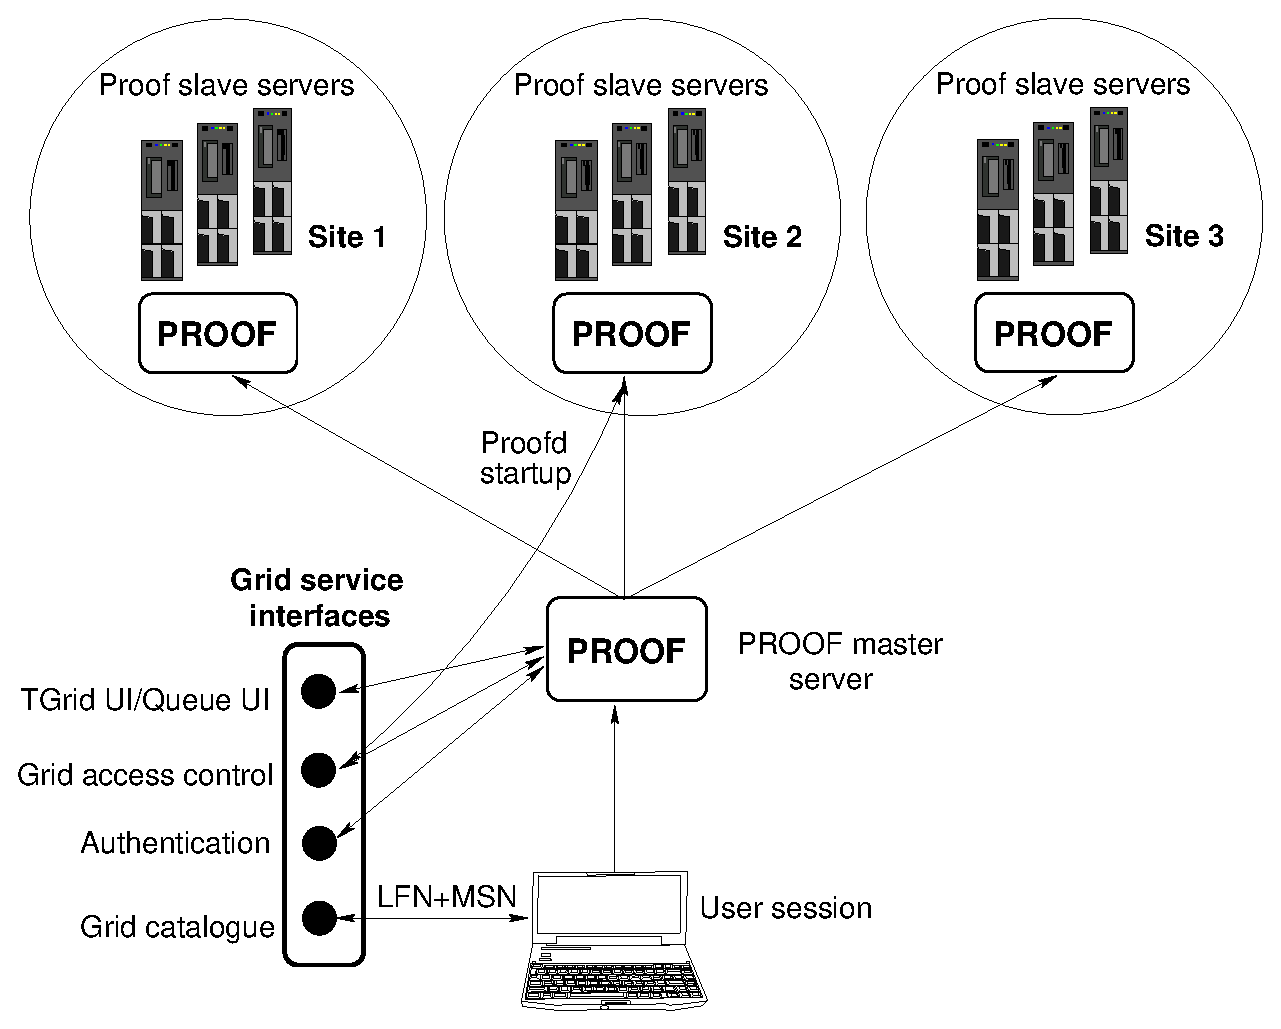
\includegraphics[width=11.5cm]{picts/alienfig7}
  \caption{Setup and interaction with the \grid middleware of a user 
    PROOF session distributed over many computing centers.} 
  \label{CH3Fig:alienfig7}
\end{figure}

% -----------------------------------------------------------------------------

\subsection{Analysis tools}

This section is devoted to the existing analysis tools in \ROOT and
\ilcroot. As discussed in the introduction, some very broad
analysis tasks include the search for some rare events (in this case the
physicist tries to maximize the signal-over-background ratio), or
measurements where it is important to maximize the signal
significance. The tools that provide possibilities to apply certain
selection criteria and to find the interesting combinations within
a given event are described below. Some of them are very general and are
used in many different places, for example the statistical
tools. Others are specific to a given analysis.

\subsubsection{Statistical tools}

Several commonly used statistical tools are available in
\ROOT\cite{ROOT}. \ROOT provides 
classes for efficient data storage and access, such as trees
and ntuples. The
ESD information is organized in a tree, where each event is a separate
entry. This allows a chain of the ESD files to be made and the
elaborated selector mechanisms to be used in order to exploit the PROOF
services. The tree classes
permit easy navigation, selection, browsing, and visualization of the
data in the branches. 

\ROOT also provides histogramming and fitting classes, which are used 
for the representation of all the one- and multi-dimensional
distributions, and for extraction of their fitted parameters. \ROOT provides
an interface to powerful and robust minimization packages, which can be 
used directly during some special parts of the analysis. A special
fitting class allows one to decompose an experimental histogram as a
superposition of source histograms.

\ROOT also has a set of sophisticated statistical analysis tools such as
principal component analysis, robust estimator, and neural networks.
The calculation of confidence levels is provided as well.

Additional statistical functions are included in \texttt{TMath}.

\subsubsection{Calculations of kinematics variables}

The main \ROOT physics classes include 3-vectors and Lorentz
vectors, and operations
such as translation, rotation, and boost. The calculations of
kinematics variables 
such as transverse and longitudinal momentum, rapidity,
pseudorapidity, effective mass, and many others are provided as well.


\subsubsection{Geometrical calculations}

There are several classes which can be used for
measurement of the primary vertex: \texttt{IlcITSVertexerZ},
\texttt{IlcITSVertexerIons}, \texttt{IlcITSVertexerTracks}, etc. A fast estimation of the {\it z}-position can be
done by \texttt{IlcITSVertexerZ}, which works for both lead--lead
and proton--proton collisions. An universal tool is provided by
\texttt{IlcITSVertexerTracks}, which calculates the position and
covariance matrix of the primary vertex based on a set of tracks, and
also estimates the $\chi^2$ contribution of each track. An iterative
procedure can be used to remove the secondary tracks and improve the
precision. 

Track propagation to the primary vertex (inward) is provided in
IlcESDtrack.

The secondary vertex reconstruction in case of ${\rm V^0}$ is provided by
\texttt{IlcV0vertexer}, and in case of cascade hyperons by
\texttt{IlcCascadeVertexer}. 
\texttt{IlcITSVertexerTracks} can be used to find secondary
vertexes close to the primary one, for example decays of open charm
like ${\rm D^0 \to K^- \pi^+}$ or ${\rm D^+ \to K^- \pi^+ \pi^+}$. All
the vertex 
reconstruction classes also calculate distance of closest approach (DCA)
between the track and the vertex.

The calculation of impact parameters with respect to the primary vertex
is done during the reconstruction and the information is available in
\texttt{IlcESDtrack}. It is then possible to recalculate the
impact parameter during the ESD analysis, after an improved determination
of the primary vertex position using reconstructed ESD tracks.

\subsubsection{Global event characteristics}

The impact parameter of the interaction and the number of participants
are estimated from the energy measurements in the ZDC. In addition,
the information  from the FMD, PMD, and T0 detectors is available. It
gives a valuable estimate of the event multiplicity at high rapidities
and permits global event characterization. Together with the ZDC
information it improves the determination of the impact parameter,
number of participants, and number of binary collisions.

The event plane orientation is calculated by the \texttt{IlcFlowAnalysis} class.

\subsubsection{Comparison between reconstructed and simulated parameters}

The comparison between the reconstructed and simulated parameters is
an important part of the analysis. It is the only way to estimate the
precision of the reconstruction. Several example macros exist in
\ilcroot and can be used for this purpose: \texttt{IlcTPCComparison.C},
\texttt{IlcITSComparisonV2.C}, etc. As a first step in each of these
macros the list of so-called `good tracks' is built. The definition of
a good track is explained in detail in the ITS\cite{CH6Ref:ITS_TDR} and 
TPC\cite{CH6Ref:TPC_TDR} Technical Design
Reports.  The essential point is that the track
goes through the detector and can be reconstructed. Using the `good
tracks' one then estimates the efficiency of the reconstruction and
the resolution.

Another example is specific to the MUON arm: the \texttt{MUONRecoCheck.C}
macro compares the reconstructed muon tracks with the simulated ones.

There is also the possibility to calculate directly the resolutions without
additional requirements on the initial track. One can use the
so-called track label and retrieve the corresponding simulated
particle directly from the particle stack (\texttt{IlcStack}).

\subsubsection{Event mixing}

One particular analysis approach in heavy-ion physics is the
estimation of the combinatorial background using event mixing. Part of the
information (for example the positive tracks) is taken from one
event, another part (for example the negative tracks) is taken from
a different, but 
`similar' event. The event `similarity' is very important, because
only in this case the combinations produced from different events
represent the combinatorial background. Typically `similar' in
the example above means with the same multiplicity of negative
tracks. One may require in addition similar impact parameters of the
interactions, rotation of the tracks of the second event to adjust the
event plane, etc. The possibility for event mixing is provided in
\ilcroot by the fact that the ESD is stored in trees and one can chain
and access simultaneously many ESD objects. Then the first pass would
be to order the events according to the desired criterion of
`similarity' and to use the obtained index for accessing the `similar'
events in the embedded analysis loops. An example of event mixing is
shown in Fig.~\ref{CH6Fig:phipp}. The background distribution has been
obtained using `mixed events'. The signal distribution has been taken
directly from the \MC simulation. The `experimental distribution' has
been produced by the analysis macro and decomposed as a
superposition of the signal and background histograms.

\begin{figure}[htb]
  \centering
  \includegraphics*[width=120mm]{picts/phipp}
  \caption{Mass spectrum of the ${\rm \phi}$ meson candidates produced
    inclusively in the proton--proton interactions.}
  \label{CH6Fig:phipp}
\end{figure}


\subsubsection{Analysis of the High-Level Trigger (HLT) data}

This is a specific analysis which is needed in order to adjust the cuts
in the HLT code, or to estimate the HLT
efficiency and resolution. \ilcroot provides a transparent way of doing
such an analysis, since the HLT information is stored in the form of ESD
objects in a parallel tree. This also helps in the monitoring and
visualization of the results of the HLT algorithms.


%\vspace{-0.1cm}
\subsubsection{EVE -- Event Visualization Environment}

EVE is composed of:
\begin{enumerate}
\item small application kernel;
\item graphics classes with editors and OpenGL renderers;
\item CINT scripts that extract data, fill graphics classes and register
   them to the application.
\end{enumerate}

The framework is still evolving ... some things might not work as expected.

\underline{Usage:}

\begin{enumerate}
\item Initialize ILC environment.
\item Spawn 'ilceve' executable and invoke the ilceve\_init.C macro,
  for example:

To load first event from current directory:
\begin{lstlisting}[language=sh]
   # ilceve  ilceve\_init.C 
\end{lstlisting}
To load 5th event from directory /data/my-pp-run:
\begin{lstlisting}[language=sh]
   # ilceve 'ilceve\_init.C("/data/my-pp-run", 5)' 
\end{lstlisting}
Interactively:
\begin{lstlisting}[language=sh]
   # ilceve
   root[0] .L ilceve\_init.C
   root[1] ilceve\_init("/somedir")
\end{lstlisting}

\item Use GUI or CINT command-line to invoke further visualization macros.
\item To navigate the events use macros 'event\_next.C' and 'event\_prev.C'.
   These are equivalent to the command-line invocations:
\begin{lstlisting}[language=sh]
   root[x] Ilceve::gEvent->NextEvent()
\end{lstlisting}
or
\begin{lstlisting}[language=sh]
   root[x] Ilceve::gEvent->PrevEvent()
\end{lstlisting}
The general form to go to event via its number is:
\begin{lstlisting}[language=sh]
   root[x] Ilceve::gEvent->GotoEvent(<event-number>)
\end{lstlisting}
\end{enumerate}

See files in EVE/ilc-macros/. For specific uses these should be
edited to suit your needs.

\underline{Directory structure}

EVE is split into two modules: REVE (ROOT part, not dependent on
IlcROOT) and ILCEVE (ILC specific part). For the time being both
modules are kept in IlcROOT CVS.

Ilceve/ and Reve/ -- sources

macros/		  -- macros for bootstraping and internal steering\\
ilc-macros/	  -- macros for ILC visualization\\
ilc-data/	  -- data files used by ILC macros\\
test-macros/      -- macros for tests of specific features; usually one needs
                     to copy and edit them\\
bin/, Makefile and make\_base.inc are used for stand-alone build of the
packages.\\

\underline{Notes}

\begin{enumerate}
\item Problems with macro-execution

A failed macro-execution can leave CINT in a poorly defined state that
prevents further execution of macros. For example:

\begin{lstlisting}[language=sh]
  Exception Reve::Exc_t: Event::Open failed opening ILC ESDfriend from
  '/ilc-data/coctail_10k/IlcESDfriends.root'.

  root [1] Error: Function MUON_geom() is not defined in current scope  :0:
  *** Interpreter error recovered ***
  Error: G__unloadfile() File "/tmp/MUON_geom.C" not loaded  :0:
\end{lstlisting}

'gROOT$\to$Reset()' helps in most of the cases.
\end{enumerate}

% ------------------------------------------------------------------------------

\vspace{-0.2cm}
\subsection{Existing analysis examples in \ilcroot}

There are several dedicated analysis tools available in \ilcroot. Their results
were used in the Physics Performance Report and described in
ILC internal notes. There are two main classes of analysis: the
first one based directly on ESD, and the second one extracting first
AOD, and then analyzing it.

\begin{itemize}
\item\textbf{ESD analysis }

  \begin{itemize}
  \item[ ] \textbf{${\rm V^0}$ and cascade reconstruction/analysis}

    The ${\rm V^0}$ candidates
    are reconstructed during the combined barrel tracking and stored in 
    the ESD object.  The following criteria are used for the selection:
    minimal-allowed impact parameter (in the transverse plane) for each
    track; maximal-allowed DCA between the two tracks;  maximal-allowed
    cosine of the 
    ${\rm V^0}$ pointing angle 
    (angle between the momentum vector of the particle combination
    and the line connecting the production and decay vertexes);  minimal
    and maximal radius of the fiducial volume; maximal-allowed ${\rm
      \chi^2}$. The 
    last criterion requires the covariance matrix of track parameters,
    which is available only in \texttt{IlcESDtrack}. The reconstruction
    is performed by \texttt{IlcV0vertexer}. This class can be used also
    in the analysis. An example of reconstructed kaons taken directly
    from the ESDs is shown in Fig.\ref{CH6Fig:kaon}. 

    \begin{figure}[th]
      \centering
      \includegraphics*[width=120mm]{picts/kaon}
      \caption{Mass spectrum of the ${\rm K_S^0}$ meson candidates produced
        inclusively in the \mbox{Pb--Pb} collisions.}
      \label{CH6Fig:kaon}
    \end{figure}

    The cascade hyperons are reconstructed using the ${\rm V^0}$ candidate and
    `bachelor' track selected according to the cuts above. In addition,
    one requires that the reconstructed ${\rm V^0}$ effective mass belongs to
    a certain interval centered in the true value.  The reconstruction
    is performed by \texttt{IlcCascadeVertexer}, and this class can be
    used in the analysis.

  \item[ ] \textbf{Open charm}

    This is the second elaborated example of ESD
    analysis. There are two classes, \texttt{IlcD0toKpi} and
    \texttt{IlcD0toKpiAnalysis}, which contain the corresponding analysis
    code. The decay under investigation is ${\rm D^0 \to K^- \pi^+}$ and its
    charge conjugate. Each ${\rm D^0}$ candidate is formed by a positive and
    a negative track, selected to fulfill the following requirements:
    minimal-allowed track transverse momentum, minimal-allowed track
    impact parameter in the transverse plane with respect to the primary
    vertex. The selection criteria for each combination include
    maximal-allowed distance of closest approach between the two tracks,
    decay angle of the kaon in the ${\rm D^0}$ rest frame in a given region,
    product of the impact parameters of the two tracks larger than a given value,
    pointing angle between the ${\rm D^0}$ momentum and flight-line smaller than
    a given value. The particle
    identification probabilities are used to reject the wrong
    combinations, namely  ${\rm (K,K)}$ and ${\rm (\pi,\pi)}$, and to enhance the
    signal-to-background ratio at low momentum by requiring the kaon
    identification. All proton-tagged tracks are excluded before the
    analysis loop on track pairs.  More details can be found in
    Ref.\cite{CH6Ref:Dainese}.

  \item[ ] \textbf{Quarkonia analysis}

    Muon tracks stored in the ESD can be analyzed for example by the macro
    \texttt{MUONmassPlot\_ESD.C}.
    This macro performs an invariant-mass analysis of muon unlike-sign pairs
    and calculates the combinatorial background.
    Quarkonia \pt and rapidity distribution are built for \Jpsi and \Ups.
    This macro also performs a fast single-muon analysis: \pt,
    rapidity, and 
    ${\rm \theta}$ vs ${\rm \varphi}$ acceptance distributions for positive
    and negative muon 
    tracks with a maximal-allowed ${\rm \chi^2}$.

  \end{itemize}

  % \newpage
\item\textbf{AOD analysis}

{\bf OBSOLETE}

  Often only a small subset of information contained in the ESD
  is needed to perform an analysis. This information
  can be extracted and stored in the AOD format in order to reduce
  the computing resources needed for the analysis.

  The AOD analysis framework implements a set of tools like data readers,
  converters, cuts, and other utility classes.
  The design is based on two main requirements: flexibility and common
  AOD particle interface. This guarantees that several analyses can be
  done in sequence within the same computing session.

  In order to fulfill the first requirement, the analysis is driven by the
  `analysis manager' class and particular analyses are added to it.
  It performs the loop over events, which are delivered by an
  user-specified reader. This design allows the analyses to be ordered
  appropriately  if some  of them depend on the results of the others.

  The cuts are designed to provide high flexibility
  and performance. A two-level architecture has been adopted
  for all the cuts (particle, pair and event). A class representing a cut
  has a list of `base cuts'. Each base cut implements a cut on a
  single property or performs a logical operation (and, or) on the result of
  other base cuts.

  A class representing a pair of particles buffers all the results,
  so they can be re-used if required.

  \vspace{-0.2cm}
  \begin{itemize}
  \item[ ] \textbf{Particle momentum correlations (HBT) -- HBTAN module}

    Particle momentum correlation analysis is based on the event-mixing technique.
    It allows one to extract the signal by dividing the appropriate
    particle spectra coming from the original events by those from the
    mixed events.

    Two analysis objects are currently implemented to perform the mixing:
    the standard one and the one implementing the Stavinsky
    algorithm\cite{CH6Ref:Stavinsky}. Others can easily be added if needed.

    An extensive hierarchy of the function base classes has been implemented
    facilitating the creation of new functions.
    A wide set of the correlation, distribution and monitoring
    functions is already available in the module. See Ref.\cite{CH6Ref:HBTAN}
    for the details. 

    The package contains two implementations of weighting algorithms, used
    for correlation simulations (the first developed by Lednicky
    \cite{CH6Ref:Weights}  and the second due to CRAB \cite{CH6Ref:CRAB}), both
    based on an uniform interface.

  \item[ ] \textbf{Jet analysis}

    The jet analysis\cite{CH6Ref:Loizides} is available in the module JETAN. It has a set of
    readers of the form \texttt{IlcJetParticlesReader<XXX>}, where \texttt{XXX}
    = \texttt{ESD},
    \texttt{HLT}, \texttt{KineGoodTPC}, \texttt{Kine}, derived from the base class
    \texttt{IlcJetParticlesReader}. These
    provide an uniform interface to
    the information from the 
    kinematics tree, from HLT, and from the ESD. The first step in the
    analysis is the creation of an AOD object: a tree containing objects of
    type \texttt{IlcJetEventParticles}. The particles are selected using a
    cut on the minimal-allowed transverse momentum. The second analysis
    step consists of jet finding. Several algorithms are available in the
    classes of the type \texttt{Ilc<XXX>JetFinder}.
    An example of AOD creation is provided in
    the \texttt{createEvents.C} macro. The usage of jet finders is illustrated in
    \texttt{findJets.C} macro.


  \item[ ] \textbf{${\rm V^0}$ AODs}

    The AODs for ${\rm V^0}$ analysis contain several additional parameters,
    calculated and stored for fast access. The methods of the class {\tt
      IlcAODv0} provide access to all the geometrical and kinematics
    parameters of a ${\rm V^0}$ candidate, and to the ESD information used
    for the calculations.

    \vspace{-0.1cm}
  \item[ ] \textbf{MUON}

    There is also a prototype MUON analysis provided in
    \texttt{IlcMuonAnalysis}. It simply fills several histograms, namely
    the transverse momentum and rapidity for positive and negative muons,
    the invariant mass of the muon pair, etc.
  \end{itemize}

\end{itemize}

%%%%%%%%%%%%%%%%%%%%%%%%%%%%%%%%%%%%%%%%%%%%%%%%%%%%%%%%%%%%%% 

\newpage
%\cleardoublepage 
\section{Analysis Foundation Library}

{\bf OBSOLETE}

The result of the reconstruction chain is the Event Summary Data (ESD) 
object. It contains all the information that may
be useful in {\it any} analysis. In most cases only a small subset 
of this information is needed for a given analysis.
Hence, it is essential to provide a framework for analyses, where
user can extract only the information required and store it in 
the Analysis Object Data (AOD) format. This is to be used in all his
further analyses. The proper data preselecting allows to speed up 
the computation time significantly. Moreover, the interface of the ESD classes is
designed to fulfill the requirements of the reconstruction
code. It is inconvenient for most of analysis algorithms,
in contrary to the AOD one. Additionally, the latter one can be customized
to the needs of particular analysis, if it is only required.

We have developed the analysis foundation library that 
provides a skeleton framework for analyses, defines AOD data format
and implements a wide set of basic utility classes which facilitate 
the creation of individual analyses.
It contains classes that define the following entities:

\begin{itemize}
\item AOD event format
\item Event buffer
\item Particle(s)
\item Pair
\item Analysis manager class 
\item Base class for analyses
\item Readers 
\item AOD writer 
\item Particle cuts 
\item Pair cuts 
\item Event cuts 
\item Other utility classes 
\end{itemize}

It is designed to fulfill two main requirements:
% 
\begin{enumerate}
\item \textbf{Allows for flexibility in designing individual analyses} 
  Each analysis has its most performing solutions. The most trivial example is 
  the internal representation of a particle momentum: in some cases the Cartesian coordinate system  is preferable and in other cases - the cylindrical one.
\item \textbf{All analyses use the same AOD particle interface to access the data }
  This guarantees that analyses can be chained. It is important when
  one analysis depends on the result of the other one, so the latter one can 
  process exactly the same data without the necessity of any conversion. 
  It also lets to carry out many analyses in the same job and consequently, the 
  computation time connected with 
  the data reading, job submission, etc. can be significantly reduced.
\end{enumerate}
% ..
The design of the framework is described in detail below.


% -----------------------------------------------------------------------------

\subsection{AOD}

The \texttt{IlcAOD} class contains only the information required
for an analysis. It is not only the data format as they are
stored in files, but it is also used internally throughout the package
as a particle container.  
Currently it contains a \texttt{TClonesArray} of particles and 
data members describing the global event properties. 
This class is expected to evolve further as new analyses continue to be 
developed and their requirements are implemented. 

% -----------------------------------------------------------------------------

\subsection{Particle}

\texttt{IlcVAODParticle} is a pure virtual class that defines a particle
interface.
Each analysis is allowed to create its own particle class 
if none of the already existing ones meet its requirements. 
Of course, it must derive  from \texttt{IlcVAODParticle}. 
However, all analyses are obliged to 
use the interface defined in \texttt{IlcVAODParticle} exclusively.
If additional functionality is required, an appropriate 
method is also added to the virtual interface (as a pure virtual or an empty one).
Hence, all other analyses can be ran on any AOD, although the processing time 
might be longer in some cases (if the internal representation is not 
the optimal one).

We have implemented the standard concrete particle class 
called \texttt{IlcAODParticle}. The momentum is stored in the
Cartesian coordinates and it also has the data members 
describing the production vertex. All the PID information
is stored in two dynamic arrays. The first array contains
probabilities sorted in descending order,
and the second one  - corresponding PDG codes (Particle Data Group).
The PID of a particle is defined by the data member which is 
the index in the arrays. This solution allows for faster information
access during analysis and minimizes memory and disk space consumption.


% -----------------------------------------------------------------------------

\subsection{Pair}

The pair object points to two particles and implements
a set of methods for the calculation of the  pair properties.
It buffers calculated values and intermediate
results for performance reasons. This solution applies to
quantities whose computation is time consuming and
also to quantities with a high reuse probability. A
Boolean flag is used to mark the variables already calculated. 
To ensure that this mechanism works properly, 
the pair always uses its own methods internally, 
instead of accessing its variables directly.

The pair object has pointer to another pair with the swapped
particles. The existence of this feature is connected to
the implementation of the mixing algorithm in the correlation 
analysis package: if particle A is combined with B, 
the pair with the swapped particles is not mixed. 
In non-identical particle analysis their order is important, and
a pair cut may reject a pair while a reversed one would be
accepted. Hence, in the analysis the swapped pair is also tried 
if a regular one is rejected. In this way the buffering feature is
automatically used also for the swapped pair.

% -----------------------------------------------------------------------------

\subsection{Analysis manager class and base class}

The {\it analysis manager} class (\texttt{IlcRunAnalysis}) drives all
the process. A particular analysis, which must inherit from 
\texttt{IlcAnalysis} class, is added to it. 
The user triggers analysis by calling the \texttt{Process} method. 
The manager performs a loop over events, which are delivered by 
a reader (derivative of the \texttt{IlcReader} class, see section 
\ref{cap:soft:secReaders}).
This design allows to chain the analyses in the proper order if any 
depends on the results of the other one. 

The user can set an event cut in the manager class.
If an event is not rejected, the \texttt{ProcessEvent}
method is executed for each analysis object. 
This method requires two parameters, namely pointers to 
a reconstructed and a simulated event. 

The events have a parallel structure, i.e. the corresponding
reconstructed particles and simulated particles have always the same index.
This allows for easy implementation of an analysis where both
are required, e.g. when constructing residual distributions.
It is also very important in correlation simulations 
that use the weight algorithm\cite{CH6Ref:Weights}. 
By default, the pointer to the simulated event is null, 
i.e. like it is in the experimental data processing.

An event cut and a pair cut can be set in \texttt{IlcAnalysis}.
The latter one points two particle cuts, so
an additional particle cut data member is redundant
because the user can set it in this pair cut.

\texttt{IlcAnalysis} class has the feature that allows to choose
which data the cuts check:
\begin{enumerate}
\item the reconstructed (default)
\item the simulated 
\item both.
\end{enumerate}
% 
It has four pointers to the  method (data members):
\begin{enumerate}
\item \texttt{fkPass1} -- checks a particle, the cut is defined by the 
  cut on the first particle in the pair cut data member
\item \texttt{fkPass2} -- as above, but the cut on the second particle is used
\item \texttt{fkPass}  -- checks a pair
\item \texttt{fkPassPairProp} -- checks a pair, but only two particle properties
  are considered
\end{enumerate}
Each of them has two parameters, namely pointers to 
reconstructed and simulated particles or pairs.
The user switches the behavior with the
method that sets the above pointers to the appropriate methods. 
We have decided to implement
this solution because it performs faster than the simpler one that uses
boolean flags and "if" statements. These cuts are used mostly inside 
multiply nested loops, and even a small performance gain transforms 
into a noticeable reduction of the overall computation time.
In the case of an event cut, the simpler solution was applied.
The \texttt{Rejected} method is always used to check events.
A developer of the analysis code must always use this method and 
the pointers to methods itemized above to benefit from this feature.

% -----------------------------------------------------------------------------

\subsection{Readers}
\label{cap:soft:secReaders}

A Reader is the object that provides data far an analysis.
\texttt{IlcReader} is the base class that defines a pure virtual
interface. 

A reader may stream the reconstructed and/or the 
simulated data. Each of them is stored in a separate AOD.
If it reads both, a corresponding reconstructed and 
simulated particle have always the same index. 

Most important methods for the user are the following:
\begin{itemize}
\item   \texttt{Next} -- It triggers reading of a next event. It returns 
  0 in case of success and 1 if no more events 
  are available.
\item   \texttt{Rewind} --  Rewinds reading to the beginning
\item   \texttt{GetEventRec} and \texttt{GetEventSim} --  They return 
  pointers to the reconstructed and the simulated events respectively.
\end{itemize}

The base reader class implements functionality for
particle filtering at a reading level. A user can set any
number of particle cuts in a reader and the particle is
read if it fulfills the criteria defined by any of them.
Particularly, a particle type is never certain and the readers
are constructed in the way that all the PID hypotheses (with non-zero 
probability) are verified.
In principle, a track can be read with more than one mass 
assumption.
For example, consider a track
which in 55\% is a pion and in 40\% a kaon, and a user wants to read 
all the pions and kaons with the PID probabilities higher then 
50\% and 30\%, respectively. In such cases two particles 
with different PIDs are added to AOD. 
However, both particle have the same Unique Identification 
number (UID) so it can be easily checked that in fact they are 
the same track.

% Multiple File Sources
\texttt{IlcReader} implements the feature that allows to specify and manipulate 
multiple data sources, which are read sequentially. 
The user can provide a list of directory names where the data are searched. 
The \texttt{ReadEventsFromTo} method allows to limit the range of events that are read
(e.g. when only one event of hundreds stored in an AOD is of interest).
% Event Buffering
\texttt{IlcReader} has the switch that enables event buffering, 
so an event is not deleted and can be quickly accessed if requested again.

% Blending
Particles within an event are frequently sorted in some way, e.g.
the particle trajectory reconstruction provides tracks sorted according
to their transverse momentum. This leads to asymmetric 
distributions where they are not expected. The user can request the
reader to randomize the particle order with \texttt{SetBlend} method.

% Writing AOD
The AOD objects can be written to disk with the \texttt{IlcReaderAOD}
using the static method \texttt{WriteAOD}. As the first
parameter user must pass the pointer to another reader that 
provides AOD objects. Typically it is \texttt{IlcReaderESD},
but it also can be other one, f.g. another \texttt{IlcReaderAOD} 
(to filter out the desired particles from the already existing AODs).

Inside the file, the AODs are stored in a \texttt{TTree}.
Since the AOD stores particles in the clones array, and many particles
formats are allowed, the reading and writing is not straight forward.
The user must specify what is the particle format to be stored on disk,
because in a general case the input reader can stream AODs with not consistent
particle formats. Hence, the careful check must be done, because storing 
an object of the different type then it was specified in the tree leads
to the inevitable crash. If the input AOD has the different particle type then
expected it is automatically converted. Hence, this method can be also used
for the AOD type conversion.

% -----------------------------------------------------------------------------

\subsection{AODs buffer}

Normally the readers do not buffer the events. 
Frequently an event is needed to be kept for further analysis, 
f.g. if uncorrelated combinatorial background is computed. 
We have implemented the FIFO (First In First Out) type buffer called
\texttt{IlcEventBuffer} that caches the defined number of events.

% -----------------------------------------------------------------------------

\subsection{Cuts}

The cuts are designed to guarantee the highest flexibility 
and performance. We have implemented the same two level architecture 
for all the cuts (particle, pair and event). 
Cut object defines the ranges of many properties that a particle, a pair or 
an event may posses and it also defines a method, which performs the
necessary check. However, usually a user wants to limit
ranges of only a few properties. For speed and robustness reasons, 
the design presented in Fig.\ref{cap:soft:partcut} was developed.

The cut object has an array of pointers to
base cuts. The number of entries in the array depends 
on the number of the properties the user wants to limit. 
The base cut implements checks on a single property. 
It implements maximum and minimum values and a virtual method \texttt{Rejected} 
that performs a range check of the value returned by pure
virtual method \texttt{GetValue}. Implementation of a concrete
base cut is very easy in most cases: it is enough to
implement \texttt{GetValue} method. The ANALYSIS package
already implements a wide range of base cuts,
and the cut classes have a comfortable interface for
setting all of them. For example it is enough to invoke
the \texttt{SetPtRange(min,max)} method and behind the scenes
a proper base cut is created and configured.

The base cuts performing a logical operation (and,or) on the result of two
other base cuts are also implemented. This way the user can configure basically any
cut in a macro. Supplementary user defined base cuts can be added in the user 
provided libraries.
In case the user prefers to implement a complicated cut in a single method (class) 
he can create his base cut performing all the operations.

The pair cut in addition to an array of pointers to the base pair 
cuts it has two pointers to particle cut, one for each particle in
the pair. 

\begin{figure}
  \begin{center}
    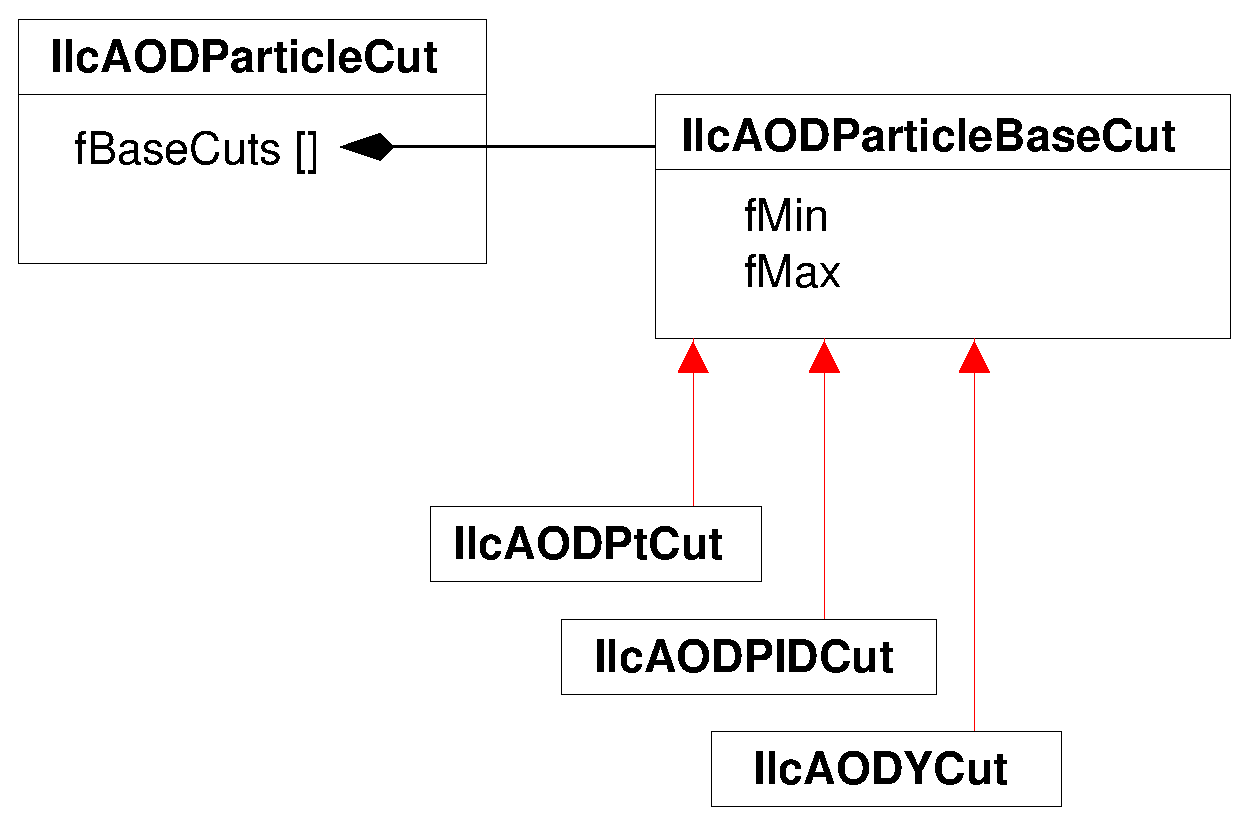
\includegraphics[width=0.4\columnwidth, origin=c]{picts/partcuts}
  \end{center}
  \caption
  {Cut classes diagram on the example of the particle cut.
    \label{cap:soft:partcut}}
\end{figure}


\subsection{Other classes}

We have developed a few classes that are used in correlation analyses,
but they can be also useful in the others. The first is the TPC cluster map,
which is the bitmap vector describing at which pad-rows a track has a cluster.
It is used by the anti-splitting algorithm in the particle correlation
analysis.

Another example is the \class{IlcTrackPoints} class, that stores 
track space coordinates at requested distances from the center of 
the detector. It is used in the particle correlation analysis
by the anti-merging cut.
The coordinates are calculated assuming the helix shape
of a track. Different options that define the way they are computed
are available. 



%%%%%%%%%%%%%%%%%%%%%%%%%%%%%%%%%%%%%%%%%%%%%%%%%%%%%%%%%%%%%%%%%%%%%%%%%%%%%%%

\newpage
%\cleardoublepage 
\section{Data input, output and exchange subsystem of IlcRoot}

This section is taken from\cite{PiotrPhD}.

A few tens of different data types is present within IlcRoot  because 
hits, summable digits, digits and clusters are characteristic for each
sub-detector. Writing all of the event data to a single file was
causing number of limitations.  
Moreover, the reconstruction chain introduces rather complicated dependences 
between different components of the framework, what is highly 
undesirable from the point of view  of software design.
In order to solve both problems, we have designed a set of classes that 
manage data manipulation i.e. storage, retrieval and exchange within 
the framework. 

It was decided to use the ``white board'' concept, which is a single
exchange object where were all data are stored and  publicly accessible.
For that purpose I have employed \textbf{TFolder} facility of ROOT.
This solution solves the problem of inter-module dependencies.

There are two most frequently occurring use-cases concerning the way a user deals with the data within the framework:
\begin{enumerate}
\item data production -- produce - \textbf{write} - \textbf{unload} (clean)
\item data processing -- \textbf{load} (retrieve) - process - \textbf{unload}
\end{enumerate}
% 
\textbf{Loader}s are the utility classes that encapsulate and 
automatize the tasks written in  bold font.
They limit the user's interaction with the I/O routines to the
necessary minimum, providing  friendly and very easy interface,
which for the use-cases considered above, consists of only 3 methods:
\begin{itemize}
\item \texttt{Load} --  retrieves the requested data to the appropriate place in the 
  white board (folder)
\item \texttt{Unload} -- cleans the data
\item \texttt{Write} -- writes the data
\end{itemize}

Such an insulation layer has number of advantages:
\begin{itemize}
\item makes the data access easier for the user. 
\item avoids the code duplication in the framework.
\item minimize the risk of a bug occurrence resulting from the improper I/O management.
  The ROOT object oriented data storage extremely simplifies the user interface,
  however, there are a few pitfalls that are frequently unknown to an 
  unexperienced user. 
\end{itemize}

To make the description more clear we need to introduce briefly  
basic concepts and the way the IlcRoot program operates. 
The basic entity is an event, i.e. all the data recorded by the 
detector in a certain time interval plus all the reconstructed information 
from these data. Ideally the data are produced by the single collision
selected by a trigger for recording. However, it may happen that the data
from the previous or proceeding events are present because the bunch 
crossing rate is higher then the maximum detector frequency (pile-up), 
or simply more than one collision occurred within one bunch crossing.

Information describing the event and the detector state is also
stored, like bunch crossing number, magnetic field, configuration, alignment, etc..,
In the case of a Monte-Carlo simulated data, information concerning the 
generator, simulation parameters is also kept. Altogether this data
is called the \textbf{header}. 

For the collisions that produce only a few tracks (best example 
are the pp collisions) it may happen that total overhead 
(the size of the header and the ROOT structures supporting object oriented 
data storage) is non-negligible in comparison with the data itself.
To avoid such situations, the possibility of storing an arbitrary number 
of events together within a \textbf{run} is required. Hence, the common data can be 
written only once per run and several events can be written to a single file.

It was decided that the data related to different detectors 
and different processing phases should be stored in different files.
In such a case only the required data need to be downloaded for an analysis.
It also allows to alter the files easily if required, 
for example when a new version of the reconstruction or simulation is needed 
to be run for a given detector. Hence, only new files are updated
and all the rest may stay untouched. It is especially important because
it is difficult to erase files in mass storage systems.
This also gives the possibility for an easy comparison of the data produced with 
competing algorithms. 

All the header data, configuration and management objects
are stored in a separate file, which is usually named gilc.root 
(for simplicity we will further refer to it as gilc).

% -----------------------------------------------------------------------------

\subsection{The ``White Board''}

The folder structure is presented in Fig.\ref{cap:soft:folderstruct}.
It is subdivided into two parts:
\begin{itemize}
\item \textbf{event data} that have the scope of single event 
\item \textbf{static data} that do not change from event to event, 
  i.e. geometry and alignment, calibration, etc.
\end{itemize}

During startup of IlcRoot the skeleton structure of the ILC white 
board is created.  The \texttt{IlcConfig} class (singleton) provides all the 
functionality that is needed to construct the folder structures.

An event data are stored under a single sub-folder (event folder) named as 
specified by the user when opening a session (run). Many sessions can be 
opened at the same time, providing that each of them has an unique event 
folder name, so they can be distinguished by this name. 
This functionality is crucial for superimposing events
on the level of the summable digits, i.e. analog detector response without the noise
contribution (the event merging). It is also useful when two events
or the same event simulated or reconstructed with a competing algorithm, 
need to be compared.

\begin{figure}
  \begin{center}
    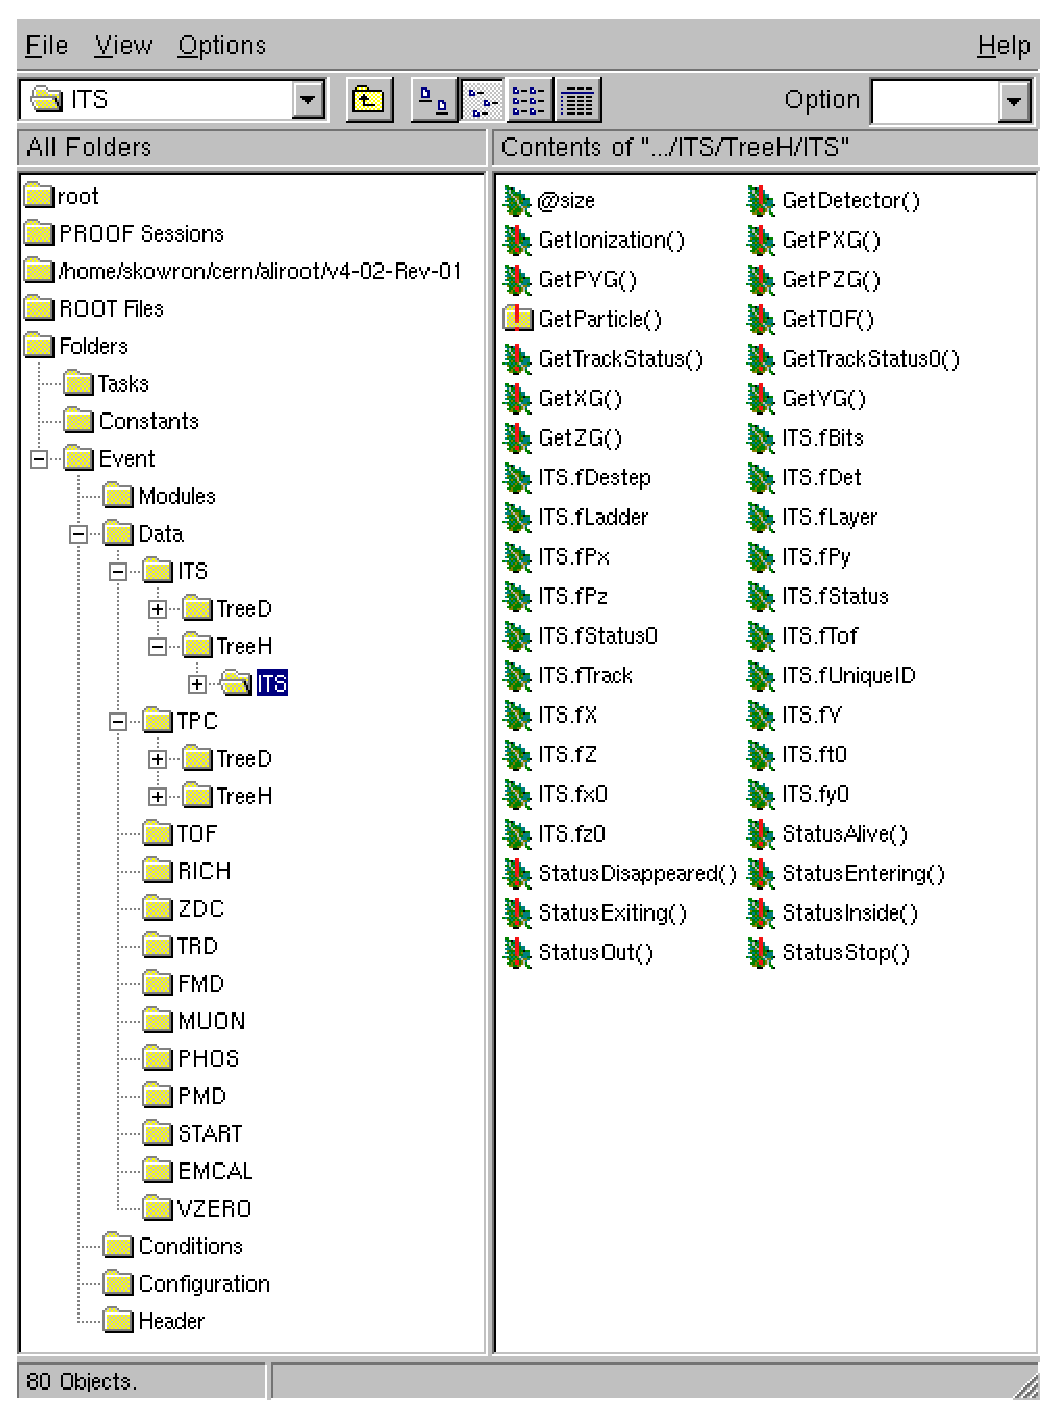
\includegraphics[width=0.8\columnwidth, origin=c]{picts/folderstruct}
  \end{center}
  \caption
  {The folders structure. An example event is mounted under ``Event'' folder.
    \label{cap:soft:folderstruct}}
\end{figure}

% -----------------------------------------------------------------------------

\subsection {Loaders}

Loaders can be represented as a four layer, tree like structure
(see Fig.\ref{cap:soft:loaderdiagram}). It represents the logical structure of
the detector and the data association.
% 
\begin{figure}
  \begin{center}
    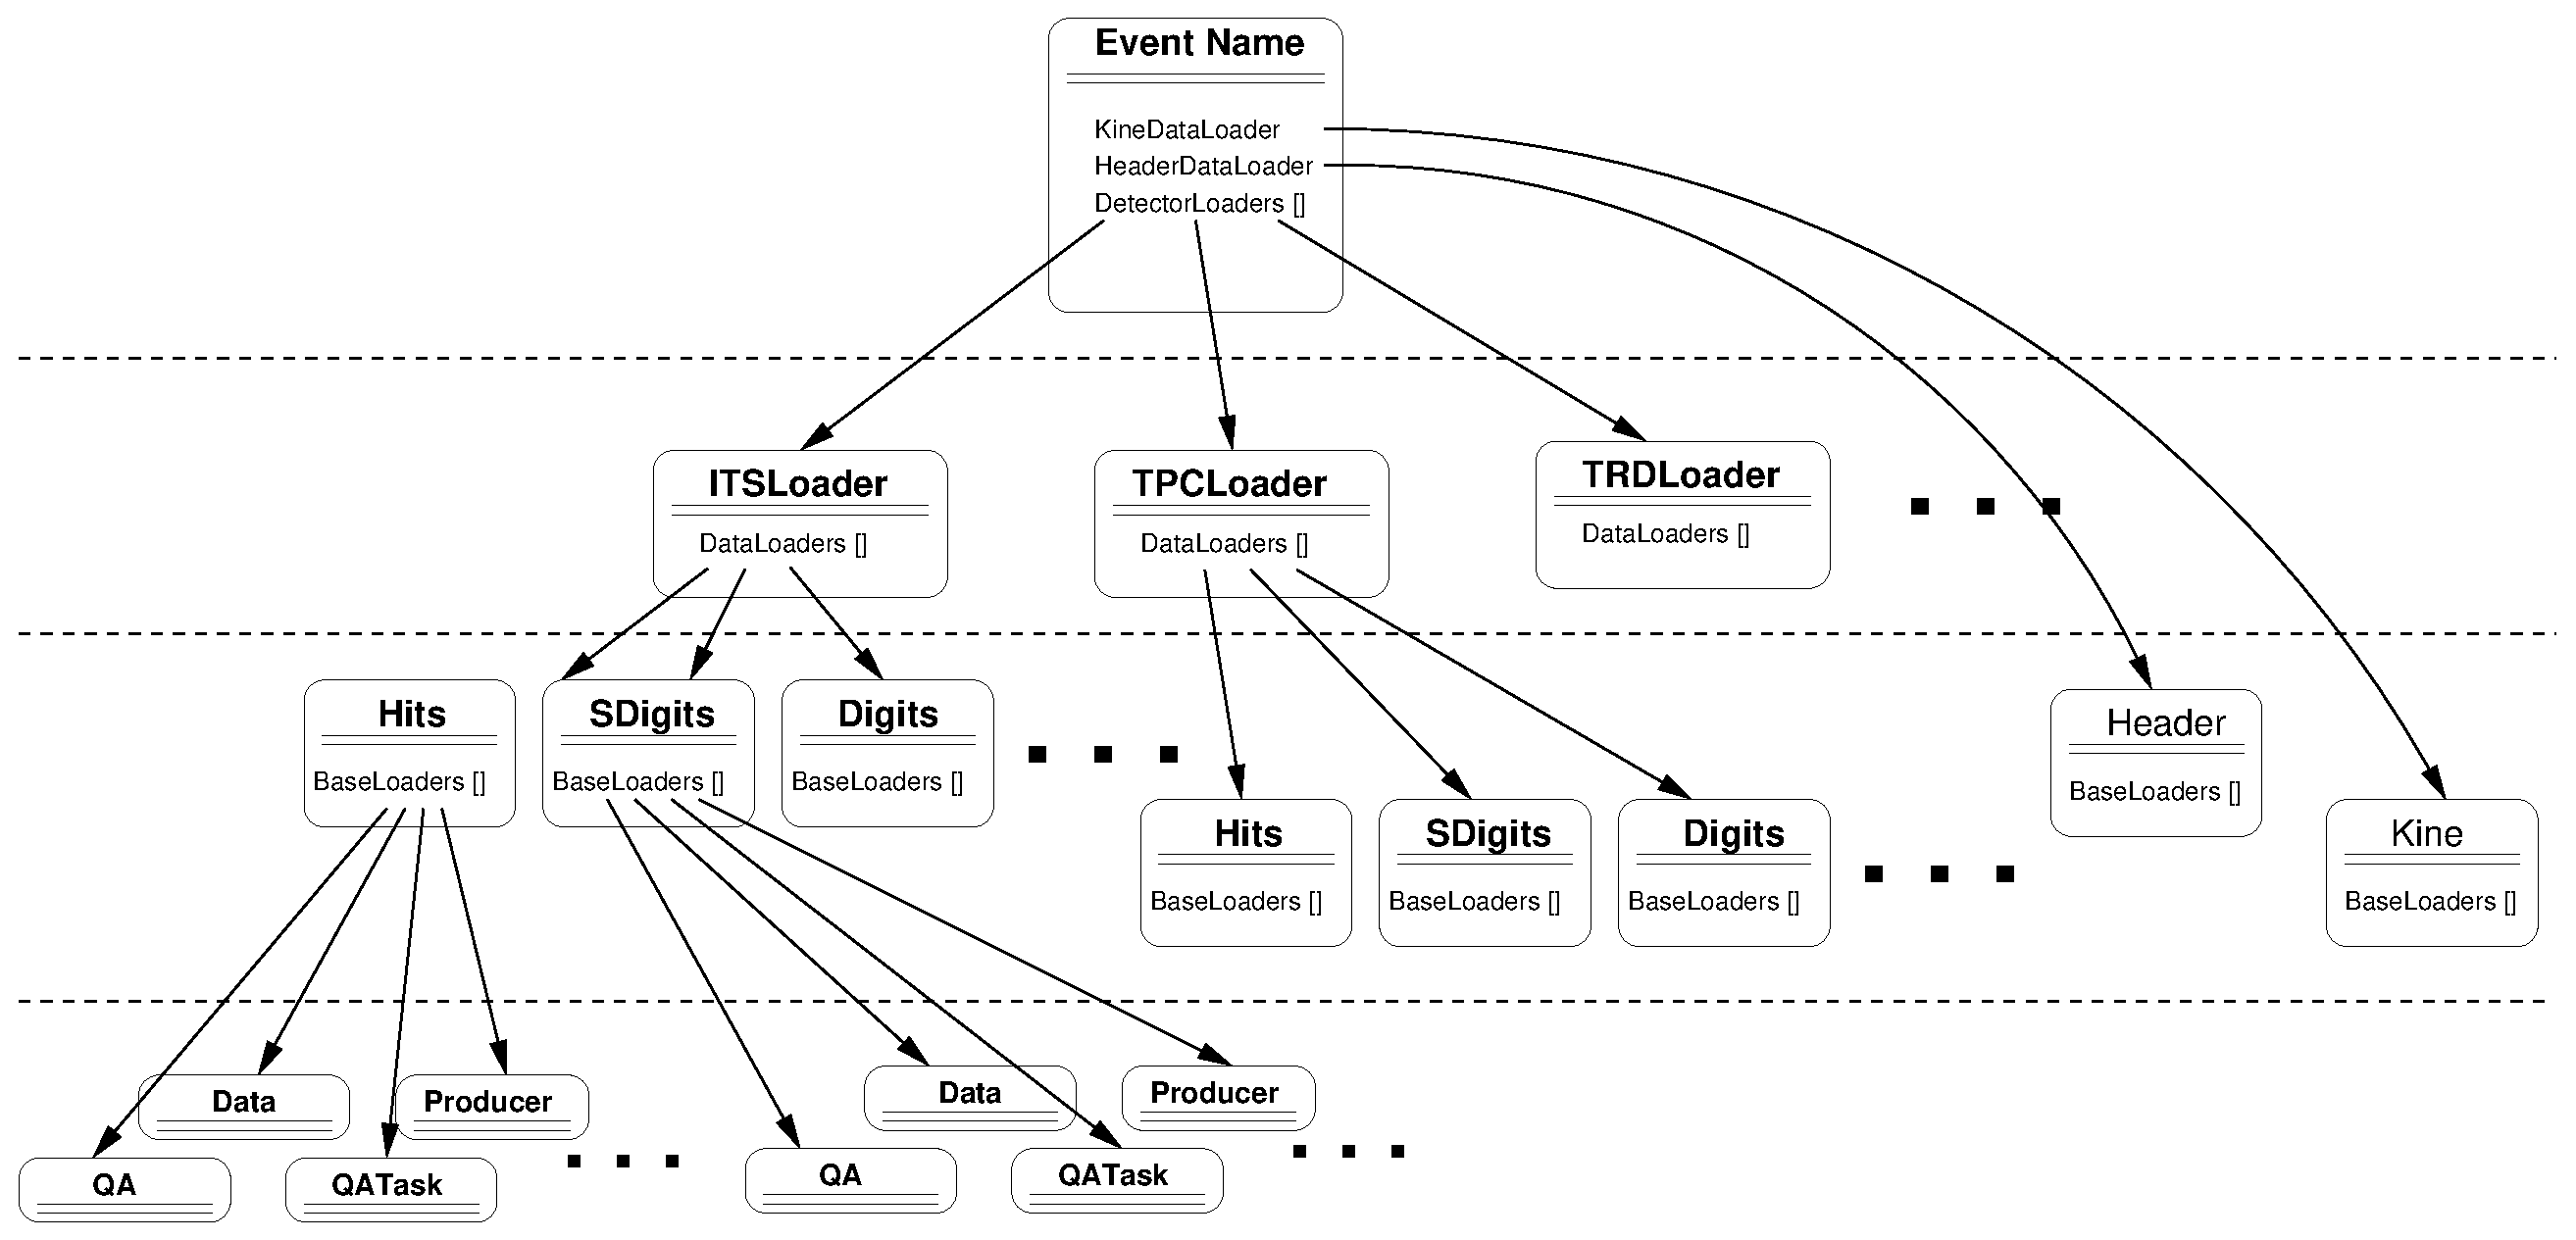
\includegraphics[width=1.0\columnwidth, origin=c]{picts/loaderdiagram}
  \end{center}
  \caption
  {Loaders diagram. Dashed lines separate layers serviced by  the different types of
    the loaders (from top): IlcRunLoder, IlcLoader, IlcDataLoader, IlcBaseLoader.
    \label{cap:soft:loaderdiagram}}
\end{figure}


\begin{enumerate}

\item \texttt{IlcBaseLoader} -- One base loader is responsible for posting 
  (finding in a file and publishing in a folder) and writing 
  (finding in a folder and putting in a file) of a single object. 
  IlcBaseLoader is a pure virtual class because writing and 
  posting depend on the type of an object. the following concrete classes are currently implemented:
  \begin{itemize}
  \item \texttt{IlcObjectLoader} -- It handles \texttt{TObject}, i.e. basically any object 
    within ROOT and IlcRoot since an object must inherit from 
    this class to be posted to the white board 
    (added to \texttt{TFolder}).

  \item \texttt{IlcTreeLoader}   -- It is the base loader for \texttt{TTrees}, 
    which requires special
    handling, because they must be always properly 
    associated with a file.

  \item \texttt{IlcTaskLoader}  -- It handles \texttt{TTask}, which need to be posted to the 
    appropriate parental \texttt{TTask} instead of \texttt{TFolder}.
  \end{itemize}
  \texttt{IlcBaseLoader} stores the name of the object it manages in
  its base class \class{TNamed} to be able
  to find it in a file or folder. The user normally does not need to use
  these classes directly and they are rather utility classes employed by
  \texttt{IlcDataLoader}.

\item \texttt{IlcDataLoader} -- It manages a single data type, for example digits for
  a detector or kinematics tree. 
  Since a few objects are normally associated with a given 
  data type (data itself, quality assurance data (QA), 
  a task that produces the data, QA task, etc.) 
  \texttt{IlcDataLoader} has an array of \texttt{IlcBaseLoaders}, 
  so each of them is responsible for each object.
  Hence, \texttt{IlcDataLoader} can be configured individually to 
  meet specific requirements of a certain data type.

  A single file contains the data corresponding to a single processing 
  phase and solely of one detector.
  By default the file is named according to the schema
  {\it Detector Name + Data Name + .root} but it can be 
  changed in run-time if needed so the data can be stored in or retrieved
  from an alternative source. When needed, 
  the user can limit the number of events stored in a single file.
  If the maximum number is exceeded, a file is closed
  and a new one is opened with the consecutive number added
  to  its name before {\it .root} suffix. Of course, 
  during the reading process, files are also automatically 
  interchanged behind the scenes and it is invisible to the user.

  The \texttt{IlcDataLoader} class performs all the tasks related 
  to  file management e.g. opening, closing, 
  ROOT directories management, etc. 
  Hence, for each data type the average file size can be 
  tuned. It is important because it is undesirable to store small 
  files on the mass storage systems and on the other hand, all file 
  systems have a maximum file size allowed.
  

\item \texttt{IlcLoader}  --    It manages all the data associated with a 
  single detector (hits, digits, summable digits, reconstructed points, etc.). 
  It has an array of \texttt{IlcDataLoaders} and each of them manages 
  a single data type. 
  
  The \texttt{IlcLoader} object is created by a class representing 
  a detector (inheriting from \texttt{IlcDetector}). 
  Its functionality can be extended and customized to the needs of a 
  particular detector by creating a specialized class that derives
  from \texttt{IlcLoader}, as it was done, for instance, for ITS or PHOS. 
  The default configuration can be 
  easily modified either in \texttt{IlcDetector::MakeLoader} 
  or by overriding the method \texttt{IlcLoader::InitDefaults}.
  
  
\item \texttt{IlcRunLoader} --  It is a main handle for data access and manipulation in
  IlcRoot. There is only one such an object in each run.
  It is always named {\it RunLoader} and stored
  on the top (ROOT) directory of a gilc file.
  
  It keeps an array of \texttt{IlcLoader}'s, one for each detector.
  It also manages the event data that are not associated with any detector
  i.e. Kinematics and Header and it utilizes \texttt{IlcDataLoader}'s
  for this purpose. 
  
  The user opens a session using a static method \texttt{IlcRunLoader::Open}.
  This method has three parameters: the file name, event folder name and mode.
  The mode can be "new" and in this case a file and a run loader are created from scratch. 
  Otherwise, a file is opened and a run loader is searched in.
  If successful, the event folder with a provided name 
  (if such does not exist yet) is created and the structure 
  presented in Fig.\ref{cap:soft:folderstruct} is created within the folder. 
  The run loader is 
  put in the event folder, so the user can always find it there
  and use it for data management.

  \texttt{IlcRunLoader} provides a simple method \texttt{GetEvent(n)} 
  to loop over events within a run. Calling it causes that all 
  currently loaded data are cleaned and the data for 
  the newly requested event are automatically posted.
  
  In order to facilitate the way the user interacts with the loaders,
  \texttt{IlcRunLoader} provides the wide set of shortcut methods. 
  For example, if digits are required to be loaded, the user can call
  \texttt{IlcRunLoader::LoadDigits("ITS TPC")}, instead of finding the appropriate
  \texttt{IlcDataLoader}'s responsible for digits for ITS and TPC, 
  and then request to load the data for each of them.
  

\end{enumerate}

\newpage
%\cleardoublepage 
\section{Calibration and alignment}


\subsection{Calibration framework}


The calibration framework is based on the following principles:

\begin{itemize}

\item the calibration and alignment database contains ROOT TObjects stored 
  into ROOT files;

\item calibration and alignment objects are RUN DEPENDENT objects;

\item the database is READ-ONLY (automatic versioning of the stored 
  objects)

\item three different data stores structures are (currently) available:
  \begin{itemize}
  \item a GRID folder containing Root files, each one containing one 
    single Root object. The Root files are created inside a directory tree 
    defined by the object's name and run validity range;
    
  \item a LOCAL folder containing Root files, each one containing one
    single Root object, with a structure similar to the Grid one;

  \item a LOCAL Root file containing one or more objects (so-called ``dump''). The 
    objects are stored into Root TDirectories defined by the
    object's name and run range.
  \end{itemize}

\item object storing and retrieval techniques are transparent to the user: 
  he/she should only specify the kind of storage he wants to use ("grid", 
  "local", "dump"). Object are stored and retrieved using the IlcCDBStorage 
  public classes:

  \begin{lstlisting}[language=C++]
    Bool_t IlcCDBStorage::Put(...) 
    and 
    IlcCDBEntry* IlcCDBStorage::Get(...) 
  \end{lstlisting}

  In addition, multiple objects can be retrieved using:

  \begin{lstlisting}[language=C++]
    TList* IlcCDBStorage::GetAll(...) (returns list of IlcCDBEntry objects).
  \end{lstlisting}

\item During object retrieval, the user has the possibility to retrieve the 
  highest version of the object or to specify a particular version by means 
  of one or more selection criteria.
\end{itemize} 

\noindent
\textbf{Features of the CDB storage classes}

% see the talk here \url{http://indico.cern.ch/conferenceDisplay.py?confId=a055286}

\begin{itemize}
\item MANAGER class IlcCDBManager. It is a singleton which handles 
  the instantiation, usage and destruction of all the storage classes. It 
  allows the instantiation of more than one storage type at a time, keeping 
  tracks of the list of active storages. The instantiation of a storage 
  element is done by means of IlcCDBManager public method GetStorage. A 
  storage element is identified by its "URI" (a string) or by its 
  "parameters". The set of parameters defining each storage is contained in 
  its specific \class{IlcCDBParam} class (\class{IlcCDBGridParam}, \class{IlcCDBLocalParam}, 
  \class{IlcCDBDumpParam}).
  
\item Versioning schema. In order to avoid version clashes when objects 
  are transferred from grid to local and vice versa, we have introduced a 
  new versioning schema. Basically the objects are defined by TWO version 
  numbers: a "Grid" version and a "Local" version (subVersion). In local 
  storage only the local version is increased, while in Grid storage only 
  the Grid version is increased. When the object is transferred from local 
  to Grid the Grid version is increased by one; when the object is 
  transferred from Grid to Local the Grid version is kept and the subVersion 
  is reset to zero. %You can find a plot of this schema on my talk (page 11). 
  
\item The container class of the object and its metadata
  (IlcCDBEntry. The metadata of the object has been divided into two  
  classes: one which contains the data used to store and retrieve the object 
  ("identity" of the object, IlcCDBId) and the other containing the metadata 
  which is not used during storage and retrieval (IlcCDBMetaData). 

  The IlcCDBId object in turn contains:
  \begin{itemize}
  \item an object describing the name (path) of the object (IlcCDBPath). The 
    path name must have a fixed, three-level directory structure: 
    "level1/level2/level3" 
  \item an object describing the run validity range of the object
    (IlcCDBRunRange)
  \item the version and subversion numbers (automatically set during storage)
  \item a string (fLastStorage) specifying from which storage the object was 
    retrieved ("new", "grid", "local", "dump")
  \end{itemize}
  
  The IlcCDBId object has two functions:
  \begin{itemize}
  \item during storage it is used to specify the path and run range of the 
    object;
  \item during retrieval it is used as a "query": it contains the
    path of the object, the required run and (if needed) the
    version and subversion to be retrieved (if version and/or
    subversion are not specified the highest ones are looked for).
  \end{itemize}
\end{itemize}

\noindent
\textbf{Some usage examples}

The following use cases are illustrated: 

\begin{itemize}
\item A pointer to the single instance of the IlcCDBManager class is obtained 
  with:

  \begin{lstlisting}[language=C++]
    IlcCDBManager::Instance()
  \end{lstlisting}

\item A storage is activated and a pointer to it is returned using the 
  \method{IlcCDBManager::GetStorage(const char* URI)} method. Here are
  some examples of how to activate a storage via an URI string. The
  URI's must have a  well defined syntax, for example (local cases):
  
  \begin{itemize}
  \item "local://DBFolder" to local storage with base directory "DBFolder" 
    created (if not existing from the working directory) 

  \item "local://\$ILC\_ROOT/DBFolder" to local storage with base directory 
    "\$ILC\_ROOT/DBFolder" (full path name)

  \item"dump://DBFile.root" to Dump storage. The file DBFile.root is looked 
    for or created in the working directory if the full path is not specified

  \item "dump://DBFile.root;ReadOnly" to Dump storage. DBFile.root is
    opened in   read only mode.
  \end{itemize}

\item Concrete examples (local case):
  
  \begin{lstlisting}[language=C++]
    IlcCDBStorage *sto = 
    IlcCDBManager::Instance()->GetStorage("local://DBFolder"):
    
    IlcCDBStorage *dump = 
    IlcCDBManager::Instance()->GetStorage("dump:///data/DBFile.root;ReadOnly"):
  \end{lstlisting}

\item Creation and storage of an object. Example of how an 
  object can be created and stored in a local database

  \begin{itemize}
  \item Let's suppose our object is an IlcZDCCalibData object (container of 
    arrays of pedestals constants), whose name is 
    "ZDC/Calib/Pedestals" and is valid for run 1 to 10. 
    
    \begin{lstlisting}[language=C++]
      IlcZDCCalibData *calibda = new IlcZDCCalibData();
      // ... filling calib data...

      // creation of the IlcCDBId object (identifier of the object)
      IlcCDBId id("ZDC/Calib/Pedestals",1,10);

      // creation and filling of the IlcCDBMetaData
      IlcCDBMetaData *md = new IlcCDBMetaData();
      md->Set... // fill meta data object, see list of setters...

      // Activation of local storage
      IlcCDBStorage *sto = 
      IlcCDBManager::Instance()->GetStorage("local://$HOME/DBFolder");

      // put object into database
      sto->Put(calibda, id, md);
    \end{lstlisting}
    The object is stored into local file: 
    \$HOME/DBFolder/ZDC/Calib/Pedestals/Run1\_10\_v0\_s0.root

  \item Examples of how to retrieve an object

    \begin{lstlisting}[language=C++]
      // Activation of local storage
      IlcCDBStorage *sto =
      IlcCDBManager::Instance()->GetStorage("local://$HOME/DBFolder");
      
      // Get the IlcCDBEntry which contains the object "ZDC/Calib/Pedestals", 
      valid for run 5, highest version
      IlcCDBEntry* entry = sto->Get("ZDC/Calib/Pedestals",5)
      // alternatively, create an IlcCDBId query and use sto->Get(query) ...

      // specifying the version: I want version 2
      IlcCDBEntry* entry = sto->Get("ZDC/Calib/Pedestals",5,2)

      // specifying version and subversion: I want version 2 and subVersion 1
      IlcCDBEntry* entry = sto->Get("ZDC/Calib/Pedestals",5,2,1)
    \end{lstlisting}

  \item Selection criteria can be also specified using 
    \method{IlcCDBStorage::AddSelection(...)} methods:

    \begin{lstlisting}[language=C++]
      // I want version 2\_1 for all "ZDC/Calib/*" objects for runs 1-100
      sto->AddSelection("ZDC/Calib/*",1,100,2,1);
      // and I want version 1\_0 for "ZDC/Calib/Pedestals" objects for runs 5-10
      sto->AddSelection("ZDC/Calib/Pedestals",5,10,1,0)
      
      IlcCDBEntry* entry = sto->Get("ZDC/Calib/Pedestals",5)
    \end{lstlisting}

    See also: \method{IlcCDBStorage::RemoveSelection(...),
      RemoveAllSelections(), PrintSelectionList()}

  \item Retrieval of multiple objects with \method{IlcCDBStorage::GetAll()}

    \begin{lstlisting}[language=C++]
      TList *list = sto->GetAll("ZDC/*",5)
    \end{lstlisting}
  \end{itemize}

\item Use of Default storage and Drain storages

  IlcCDBManager allows to set pointers to a "default storage" and to a 
  "drain storage". In particular, if the drain storage is set, all the 
  retrieved objects are automatically stored into it.

  The default storage is automatically set as the first active storage. To 
  set the default storage to another storage:

  \begin{lstlisting}[language=C++]
    IlcCDBManager::Instance()->SetDefaultStorage("uri")
  \end{lstlisting}

  The default storage can be then used by:
  \begin{lstlisting}[language=C++]
    IlcCDBEntry *entry =
    IlcCDBManager::Instance()->GetDefaultStorage()->Get(...)  
  \end{lstlisting}

  The drain storage can be set in a similar way:

  \begin{lstlisting}[language=C++]
    IlcCDBManager::Instance()->SetDrain("uri")
  \end{lstlisting}

  There are some IlcCDBManager public methods to handle the default and 
  storage methods:

  \begin{lstlisting}[language=C++]
    Bool_t 	IsDefaultStorageSet()
    void	RemoveDefaultStorage()
    Bool_t 	IsDrainSet()
    void	RemoveDrain()
  \end{lstlisting}

\item Example of how to use default and drain storage:

  \begin{lstlisting}[language=C++]
    IlcCDBManager::Instance()->SetDefaultStorage("local://$HOME/DBFolder");
    IlcCDBManager::Instance()->SetDrain("dump://$HOME/DBDrain.root");

    IlcCDBEntry *entry = 
    IlcCDBManager::Instance()->GetDefaultStorage()->Get("ZDC/Calib/Pedestals",5)
    // Retrieved entry is automatically stored into DBDrain.root !
  \end{lstlisting}

\item To destroy the IlcCDBManager instance and all the active storages:

  \begin{lstlisting}[language=C++]
    IlcCDBManager::Instance()->Destroy()
  \end{lstlisting}

 \item Create a local copy of all the alignment objects

  \begin{lstlisting}[language=C++]
    IlcCDBManager* man = IlcCDBManager::Instance();
    man->SetDefaultStorage(
      "alien://folder=/ilc/simulation/2006/PDC06/Residual/CDB/");

    man->SetDrain("local://$ILC_ROOT/CDB");
    IlcCDBStorage* sto = man->GetDefaultStorage();
    sto->GetAll("*",0);

    // All the objects are stored in $ILC_ROOT/CDB !
  \end{lstlisting}

\end{itemize}

%%%%%%%%%%%%%%%%%%%%%%%%%%%%%%%%%%%%%
\newpage
\section{The Event Tag System}

The event tag system \cite{EventTag} is designed to provide fast
preselection of 
events with the desired characteristics. This task will be performed
first of all by imposing event selection criteria within the analysis
code and then by interacting with software that is designed to provide
a file-transparent event access for analysis. The latter is an
evolution of the procedure that has already been implemented by the
STAR \cite{STAR} collaboration. 

In the next sections we will first describe the analysis scheme using
the event tag system. Then we will continue by presenting in detail
the existing event tag prototype. Furthermore, a separate section is
dedicated to the description of the two ways to create the tag files
and their integration in the whole framework \cite{CompTDR}. 

\subsection{The Analysis Scheme}

ILC collaboration intends to use a system that will reduce the time
and computing resources needed to perform an analysis by providing to
the analysis code just the events of interest as they are defined by
the users' selection criteria. Fig. \ref{analysis} gives a schematic
view of the whole analysis architecture.

\begin{figure}[ht!]
   \centering
   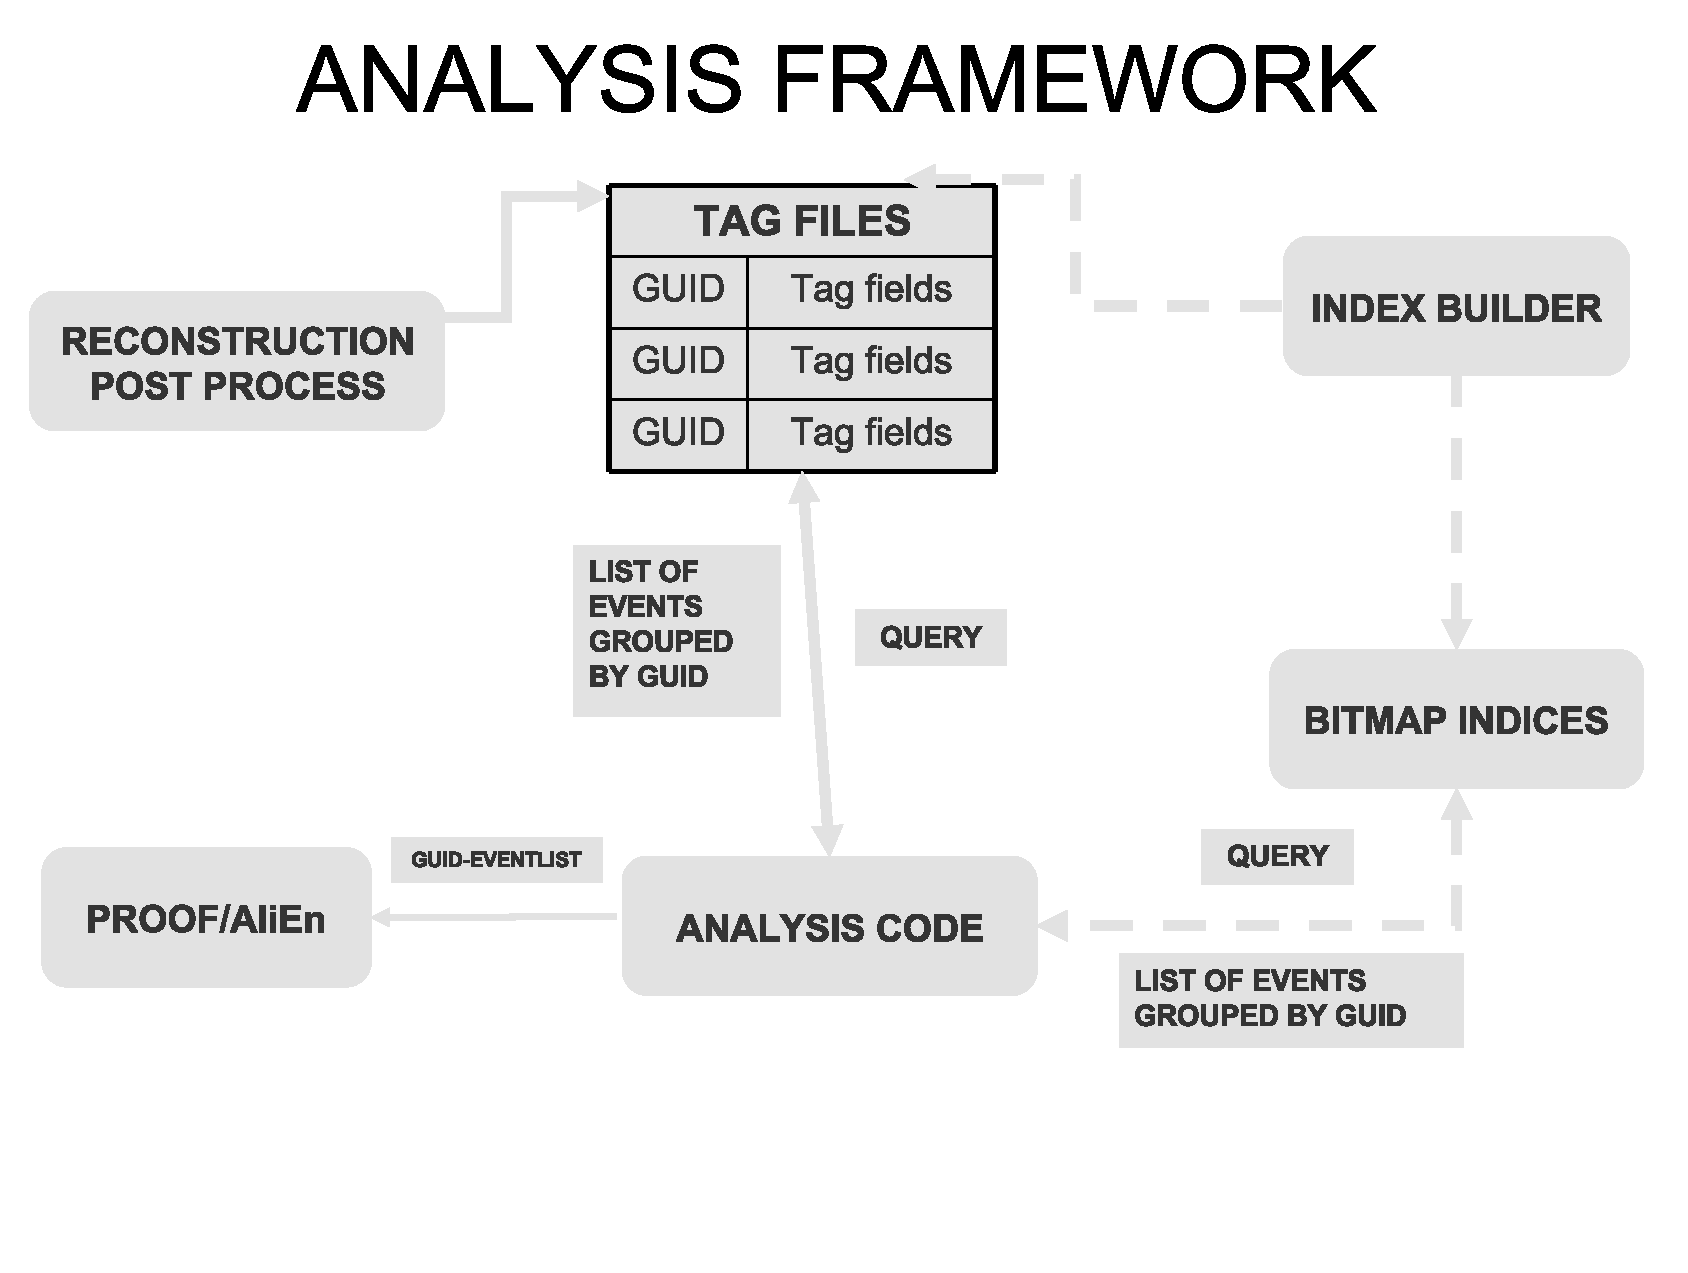
\includegraphics[width=10cm]{picts/tagana}
   \caption{The selected analysis scheme using the event tag system. }
   \label{analysis}
\end{figure}

Before describing the architecture let us first define a few terms
that are listed in this figure:

\begin{itemize}

\item User/Administrator: A typical ILC user or even the
  administrator of the system who wants to create tag files for all or
  a few ESDs \cite{CompTDR} of a run.


\item Index Builder: A code with Grid Collector \cite{GC1,GC2}
  functionality that allows the creation of compressed bitmap indices
  from the attributes listed in the tag files. This functionality will
  provide an even faster preselection.


\item Selector: The user's analysis code that derives from the
  TSelector class of ROOT \cite{RootSelector}.


\end{itemize}

The whole procedure can be summarized as follows:

The offline framework will create the tag files, which will hold
information about each Event Summary Data (ESD) file (top left box of
Fig.\ref{analysis}), as a final step of the whole reconstruction
chain. The creation of the tag files is also foreseen to be performed
by each user in a post process that will be described in the following
sections. These tag files, as will be mentioned in this note, are root
files containing trees of tag objects. Then, following the procedure
flow as it is shown in Fig. \ref{analysis}, the indexing algorithm of
the Grid Collector \cite{GC1,GC2}, the \textit{Index Builder}, will
take the produced tag files and create the compressed bitmap
indices. In parallel, the user will submit a job with some selection
criteria relevant to the corresponding analysis he/she is
performing. These selection criteria will be used in order to query
the produced compressed indices (or as it is done at the moment the
query will be on the tags themselves) and the output of the whole
procedure will be a list of \textit{TEventList} objects grouped by
\textit{GUID}, which is the file's unique identifier in the file
catalog, as it is shown in the middle box of Fig.\ref{analysis}. This
output will be forwarded to the servers that will interact with the
file catalog in order to retrieve the physical file for each
\textit{GUID} (left part of Fig. \ref{analysis}). The final result
will be passed to a selector \cite{RootSelector} that will process the
list of the events that fulfill the imposed selection criteria and
merge the output into a single object, whether this is a histogram or
a tree or any root object. 

The whole implementation implies the existence of an event tag system
that will allow the user to create the tags for each file. This event
tag system is active and has been used inside IlcRoot's framework
\cite{ilcroot} since June 2005. In the next section we will describe
this system in detail. 


\subsection{The Event Tag System}

The event tag system that has been built, intends to provide a summary
of the most useful physics information that describe each ESD to the
user. It consists of four levels of information \cite{EventTagWeb}: 

\begin{itemize}

\item Run Level: Fields that describe the run conditions and
  configurations and are retrieved from Detector Control System (DCS),
  Data Acquisition system (DAQ) and offline (Fig. \ref{sources}). 

\item LHC Level: Fields that describe the LHC condition per ILC run
  which are retrieved from the DCS (Fig. \ref{sources}). 

\item Detector Level: Fields that describe the detector configuration
  per ILC run which are retrieved from the Experimental Control
  system (ECS) (Fig. \ref{sources}). 

\item Event Level: Fields that describe each event - mainly physics
  related information and are retrieved by both offline and the grid
  file catalog (Fig. \ref{sources}). 

\end{itemize}

\begin{figure}[ht!]
    \centering
    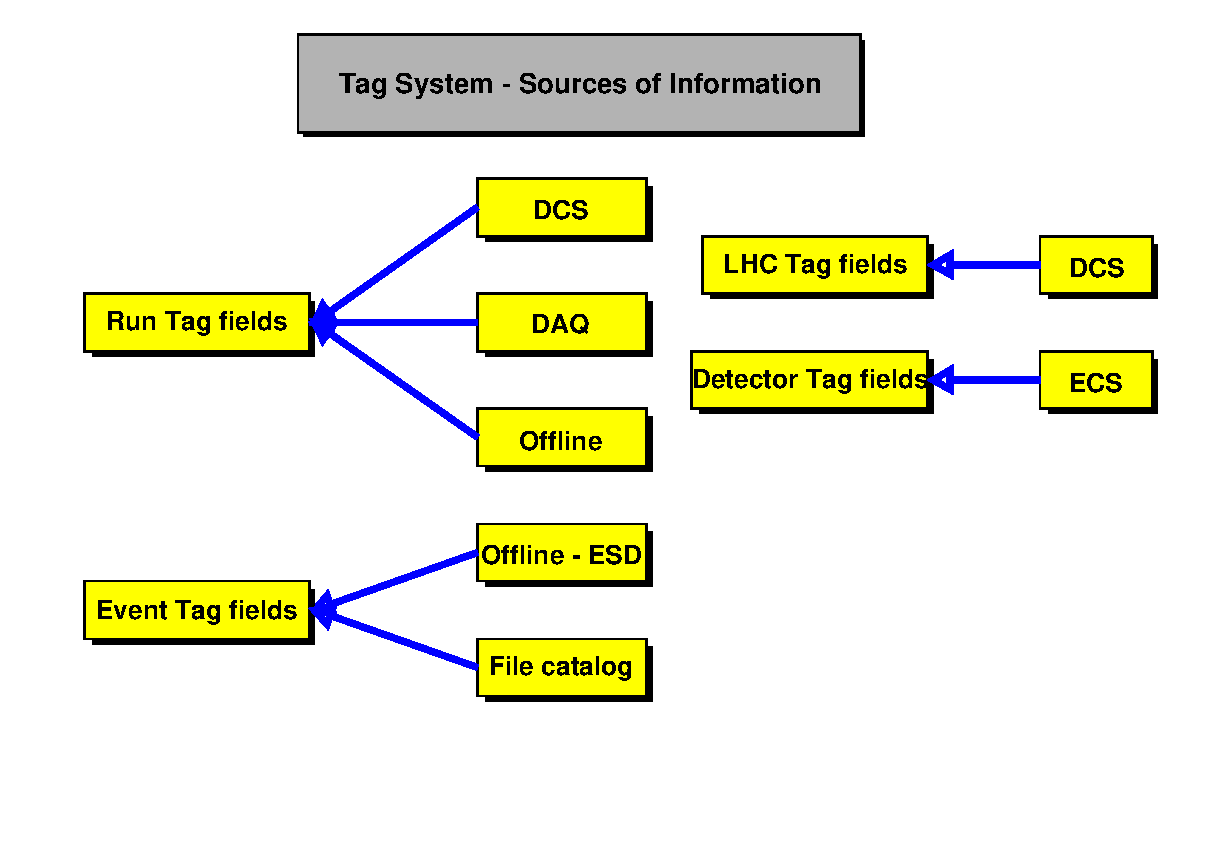
\includegraphics[width=15cm]{picts/tagsources}
    \caption{The sources of information for the different levels of the event tag system.}
    \label{sources}
\end{figure}

The corresponding classes that form this system have already been
included in IlcRoot's framework under the
\textbf{STEER} module. The output tag files will be root files having
a tree structure \cite{EventTagWeb}.

\underline{Run tags:}

The class that deals with the run tag fields is called
\class{IlcRunTag}. One \class{IlcRunTag} object is associated to
each file.

\underline{LHC tags:}

The class that deals with the LHC tag fields is called
\class{IlcLHCTag}. One \class{IlcLHCTag} object is associated to
each file.

\underline{Detector tags:}

The class that deals with the detector tag fields is called
\class{IlcDetectorTag}. The information concerning the detector
configuration per ILC run will be described in the ECS database
(Fig. \ref{sources}). One \class{IlcDetectorTag} object is associated
to each file.

\underline{Event tags:}

The class that handles the event tag fields is called
\class{IlcEventTag}. The values of these fields, as mentioned before,
will be mainly retrieved from the ESDs although there are some fields
the values of which will come from the grid file catalog. The number
of \class{IlcEventTag} objects which are associated to each file is
equal to the number of events that are stored inside the initial ESD
file.

\subsection{The Creation of the Tag Files}

As it was mentioned in a previous section, the creation of the tag
files will be the first step of the whole procedure. Two different
scenarios were decided: 

\begin{itemize}

\item \textbf{On the fly creation}: The creation of the tag file comes
  as a last step of the reconstruction procedure.  

\item \textbf{Post creation}: After the ESDs have been transfered to
  the ILC's file catalog \cite{AliEn}, every user has the
  possibility to run this post process and create his/her own tag
  files. 

\end{itemize}

\subsubsection{The on the fly creation scenario}

As mentioned before, the on the fly creation of the tag files is
implemented in such a way that the tags are filled as a last step of
the reconstruction chain. This process is treated inside the
\class{IlcReconstruction} class. Thus, exactly after the creation of
the ESD, the file is passed as an argument to the
\method{IlcReconstruction::CreateTags(TFile *file)} method. Inside
this method empty \class{IlcRunTag} and \class{IlcEventTag} objects
are created. The next step is to loop over the events listed in the
ESD file and finally fill the run and event level information. The
naming convention followed for the output tag file is:
\textbf{Run}\textbf{\textit{RunId}}.\textbf{Event}\textbf{\textit{FirstEventId}}\_\textbf{\textit{LastEventId}}.\textbf{ESD.tag.root}
\cite{EventTagWeb}. 

\subsubsection{The post creation scenario}

The post creation procedure provides the possibility to every user to
create and store the tag files at any time \cite{EventTagWeb}. The
post creation of the tag files implies the following steps: 

\begin{itemize}

\item The reconstruction code finishes and several ESD files are created. 

\item These files are stored then in ILC's file catalog \cite{AliEn}. 

\item Then the administrator or even every user for the purpose of his
  private analysis, can loop over the produced ESDs and create the
  corresponding tag files.

\item These files can either be stored locally or can be stored in the
  file catalog \cite{AliEn}.

\item As a final step, a user can choose to create a single merged tag
  file from all the previous ones.

\end{itemize}

What a user has to do in order to create the tag files using this
procedure depends on the location of the input IlcESDs.root
files. Detailed instructions on how to create tag files for each
separate case will be given in the following sections. In general a
user has to perform the following steps:

\begin{itemize}

\item Generate the input that provides information about the location
  of the IlcESDs.root files: this can be the result of a query to the
  file catalog (\emph{TGridResult} \cite{RootTGridResult} - grid
  stored ESDS, an upper level local directory - locally stored ESDs or
  even a text file - CERN Analysis Facility (CAF) stored ESDs
  \cite{CAF}.

\item Loop over the entries of the given input (\emph{TGridResult},
  \emph{local path}, \emph{text file}) and create the tag file for
  each entry.

\item Either store the files locally or in the grid's file catalog.

\item Merge the tag files into one and store it accordingly (locally
  or in the file catalog) \cite{RootApi}.

\end{itemize}

Fig. \ref{posttag} has a schematic view of these functionalities.


\begin{figure}[ht!]
   \centering
   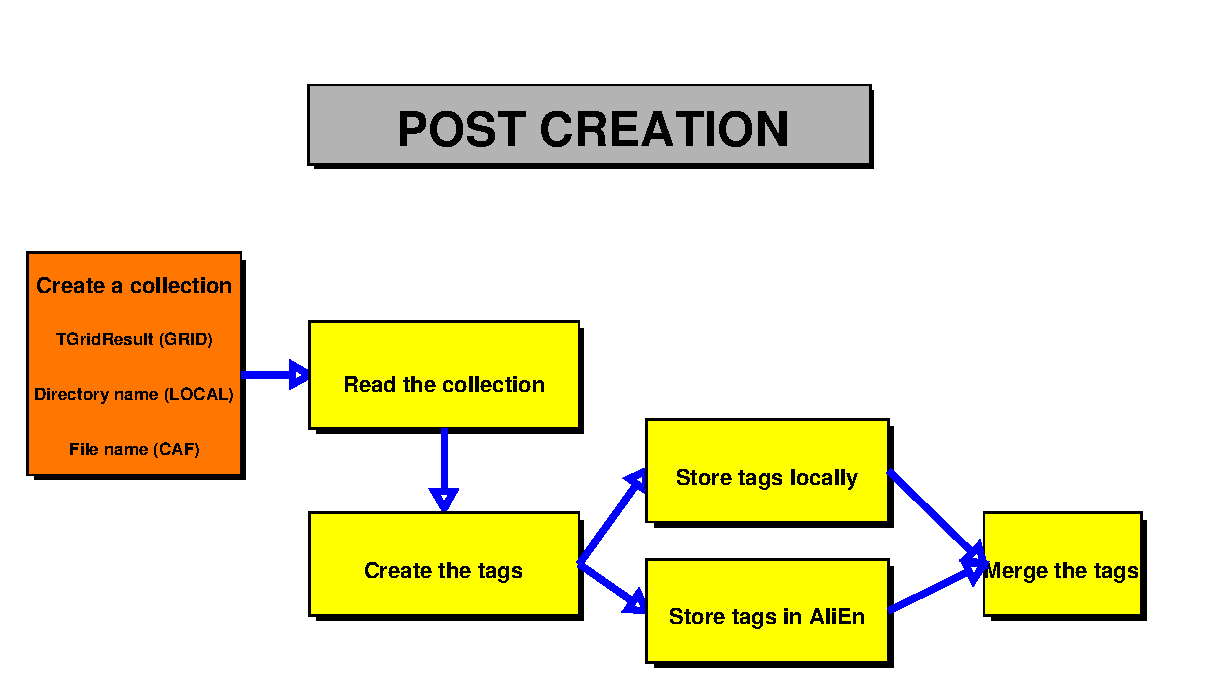
\includegraphics[width=15cm]{picts/tagpost}
   \caption{A schematic view of the architecture of the post creation of the tag files.}
   \label{posttag}
\end{figure}

The class that addresses this procedure is the \class{IlcTagCreator}. The main methods of the class and their corresponding functionalities are described in the following lines:

\begin{itemize}

\item \method{IlcTagCreator()}: The default constructor of the
  class. It is used to initialize the private members.
\item \method{void SetStorage(Int\_t storage)}: Allows the user to
  define the place where the tag files will be stored. In general
  there are two possibilities: the tags can either be stored locally
  (storage = 0) or in the file catalog (storage = 1). If the user
  defines some other value then an error message appears and the
  process is aborted.

\item \method{void SetSE(const char *se)}: This method can be used in
  the case where the files will be stored in the grid. It allows the
  user to define the desired storage element. If not selected the
  default storage element will be used.

\item \method{void SetGridPath(const char *gridpath)}: This method may
  be used in the case where the files will be stored in the grid. It
  allows the user to define the grid path under which the files will
  be stored. If not selected the tag files will be stored in the home
  directory of the user in the file catalog.

\item \method{Bool\_t ReadGridCollection(TGridResult *result)}: This
  method is used when creating tag files from ESDs that are stored in
  the file catalog. It takes as an input the result of the query to
  the file catalog \textit{TGridResult} and loops over the
  corresponding entries. For each one the
  \method{IlcTagCreator::CreateTags(TFile *f, const char* guid, const char* md5, const char*turl, Long64\_t size, Int\_t Counter)}
  protected method will be called to create the tag files that will be
  stored accordingly.

\item \method{Bool\_t ReadCAFCollection(const char* filename)}: This
  method is used when creating tag files from ESDs that are stored in
  the CERN Analysis Facility (CAF)\cite{CAF}. It takes as an input a
  text file that has all the information about the location of the
  files within the storage element of the CAF. For each one, the
  \method{IlcTagCreator::CreateTags(TFile *f, const char* filepath,
    Int\_t Counter)} protected method will be called to create the tag
  files that will be stored accordingly.

\item \method{Bool\_t ReadLocalCollection(const char* localpath)}:
  This method is used when creating tag files from ESDs that are
  stored locally. It takes as an input the upper directory where the
  ESD files are stored. The system assumes that one level down there
  are several subdirectories where the IlcESDs.root are store. The
  method searches the file system and when it finds an ESD file the
  \method{IlcTagCreator::CreateTags(TFile *f, const char* filepath, Int\_t Counter)}
 protected method will be called to create the tag
  files that will be stored accordingly.

\item \method{void CreateTag(TFile* file, const char *guid, const char *md5, const char *turl, Long64\_t size, Int\_t Counter)}:
 Protected method that is called inside the
 \method{IlcTagCreator::ReadGridCollection(TGridResult *result)}
 method. Creates the tag file and stores it locally if \method{IlcTagCreator::SetStorage(0)}
  or in AliEn if \method{IlcTagCreator::SetStorage(1)}.

\item \method{void CreateTag(TFile* file, const char *filepath, Int\_t Counter)}:
 Protected method that is called inside the
  \method{IlcTagCreator:: ReadCAFCollection(const char* filename)} or
  the \method{IlcTagCreator:: ReadLocalCollection(const char* filepath)}
 method. Creates the tag file and stores it locally if
  \method{IlcTagCreator::SetStorage(0)} or in AliEn if
  \method{IlcTagCreator::SetStorage(1)}.

\item \method{Bool\_t MergeTags()}: Chains all the tags regardless of
  the location (locally stored or in the grid) and merges them by
  creating a single tag file having a name:
  \textbf{Run}\textbf{\textit{RunId}}.\textbf{Merged}.\textbf{ESD.tag.root}.
  This file is then stored either locally or in the grid according to
  the value set in the \method{SetStorage} method.



\end{itemize}

\subsubsection{Usage of IlcRoot classes}

The following lines intend to give an example on how to use the
\textbf{IlcTagCreator} class in order to create tags. Additional
information can be found in \cite{EventTagWeb}. There are three
different cases depending on the location where the IlcESDs.root files
are stored:


\begin{itemize}

\item Locally stored IlcESDs.root files.

\item CAF stored IlcESDs.root files.

\item Grid stored IlcESDs.root files.

\end{itemize}

We will address the three different cases separately.

\underline{Locally stored IlcESDs.root}

We assume that for debugging or source code validation reasons, a user
has a few IlcESDs.root files stored locally. The files are stored
under $\$HOME/PDC06/pp$. One level down, the directory structure can
be of the form:


\begin{itemize}

\item xxx/IlcESDs.root
\item yyy/IlcESDs.root
\item zzz/IlcESDs.root

\end{itemize}

\noindent where xxx is the directory name which can be something like
\emph{Run1, Run2} etc or even the run number. In order to create the
tag files for this case we need to create an empty
\class{IlcTagCreator} object. The next step is to define whether the
produced tags will be stored locally on in the grid. If the second
option is chosen, then the user should define the SE and the
corresponding grid path where the tag files will be stored. If the
first option is chosen, then the files will be stored locally in
his/hers working directory. Finally the call of the
\method{IlcTagCreator::ReadLocalCollection(const char* filepath)}
allows the user to query the local file system and create the tag
files.


\vspace{0.2 cm}

\begin{lstlisting}[language=C++]
  //create an IlcTagCreator object
  IlcTagCreator *t = new IlcTagCreator(); 
  //Store the tag files locally
  t->SetStorage(0);
  //Query the file system, create the tags and store them
  t->ReadLocalollection(''/home/<username>/PDC06/pp'');
  //Merge the tags and store the merged file
  t->MergeTags();
\end{lstlisting}

\underline{CAF stored IlcESDs.root}

In the case where the ESD files are stored in the CAF, then we take as
an input the text file that has the information about the location of
the files in the storage element of the system \cite{EventTagWeb,
  CAF}. The next lines, where we assume that this input file is called
\emph{ESD.txt} and is located in the working directory, indicate the
steps that one has to follow:


\begin{lstlisting}[language=C++]
  //create an IlcTagCreator object
  IlcTagCreator *t = new IlcTagCreator(); 
  //Store the tag files in AliEn's file catalog
  t->SetStorage(0);
  //Read the entries of the file, create the tags and store them
  t->ReadCAFCollection(``ESD.txt'');
  //Merge the tags and store the merged file
  t->MergeTags();
\end{lstlisting}

\underline{GRID stored IlcESDs.root}

In the case where the ESD files are stored in the file catalog, then
the first thing a user needs to have is a ROOT version compiled with
AliEn support. Detailed information on how to do this, can be found in
\cite{RootApi}. Then we need to invoke the AliEn's API services
\cite{RootApi} and use as an input a query to the file catalog
(\class{TGridResult}). The following lines give an example of the
whole procedure:

 
\begin{lstlisting}[language=C++]
  //connect to AliEn's API services
  TGrid::Connect("alien://pcapiserv01.cern.ch:10000","<username>");   
  //create an IlcTagCreator object
  IlcTagCreator *t = new IlcTagCreator(); 
  //Query the file catalog and get a TGridResult
  TGridResult* result = 
  gGrid->Query("/ilc/cern.ch/user/p/pchrista/PDC06/pp/*",
  "IlcESDs.root","","");
  //Store the tag files in AliEn's file catalog
  t->SetStorage(1);
  //Define the SE where the tag files will be stored
  t->SetSE("ILC::CERN::se01");
  //Define the grid's path where the tag files will be stored
  t->SetGridPath("PDC06/Tags");
  //Read the TGridResult, create the tags and store them
  t->ReadGridCollection(result);
  //Merge the tags and store the merged file
  t->MergeTags();
\end{lstlisting}



%%%%%%%%%%%%%%%%%%%%%%%%%%%%%%%%%%%%%%%%%%%%%%%%%%%%%%%%%%%%%%%%%%%%%%%%%%%%%%%

\newpage
\appendix

\section{Kalman filter}
Kalman filtering is quite a general and  powerful method for statistical
estimations and predictions. The conditions for its 
applicability are the following. A certain `system' is
determined at any moment in time $t_k$ by a state vector $x_k$.  The state
vector varies with time according to an evolution
equation
\[ x_k = f_k(x_{k-1}) + \epsilon_k .  \]
It is supposed that $f_k$ is
a known deterministic function and $\epsilon_k$ is a random vector of intrinsic
`process noise' which has a zero mean value ($<\epsilon_k> = 0$) and a known
covariance matrix (${\rm cov}(\epsilon_k) = Q_k$). Generally, only some function
$h_k$ of the state vector can be observed, and the result of the
observation $m_k$ is
corrupted by a `measurement noise' $\delta_k$:
\[ m_k = h_k(x_k) + \delta_k. \]
The measurement noise is supposed to be unbiased ($<\delta_k> = 0$) and have a
definite covariance matrix (${\rm cov}(\delta_k) = V_k$). In many cases, the
measurement function $h_k$ can be represented by a
certain matrix $H_k$:
\[ m_k = H_kx_k + \delta_k .\]

If, at a certain time $t_{k-1}$, we are given 
some estimates of the state vector $\tilde{x}_{k-1}$ and of
its covariance matrix $\tilde{C}_{k-1} = {\rm cov}(\tilde{x}_{k-1}-x_{k-1})$,
we can extrapolate
these estimates to the next time slot $t_k$ by means of formulas
(this is called `prediction'):
\begin{eqnarray}
  \tilde{x}_k^{k-1} &=& f_k(\tilde{x}_{k-1}) \nonumber \\
  \tilde{C}_k^{k-1} &=& F_k\tilde{C}_{k-1}F_k^T + Q_k\mbox{,\ \ \ \ }
  F_k=\frac{\displaystyle\partial f_k}{\displaystyle\partial x_{k-1}} . 
  \nonumber
  % \label{pre}
\end{eqnarray}
The value of the predicted $\chi^2$ increment can be also calculated:
\begin{equation}
  (\chi^2)_k^{k-1} = (r_k^{k-1})^T(R_k^{k-1})^{-1}r_k^{k-1}\mbox{,\ \ \ \ }
  r_k^{k-1} = m_k - H_k\tilde{x}_k^{k-1}\mbox{,\ \ \ \ }
  R_k^{k-1} = V_k + H_k\tilde{C}_k^{k-1}H_k^T . 
  \nonumber
  % \label{chi}
\end{equation}
The number of degrees of freedom is equal to the dimension of the vector $m_k$.

If at the moment $t_k$, together with the results of prediction, we also
have the results of the state vector measurement, 
this additional information can be combined with the prediction  results
(this is called `filtering'). As a consequence, the estimation of the state
vector improves with respect to the previous step:
\begin{eqnarray}
  \tilde{x}_k &=& \tilde{x}_k^{k-1} + K_k(m_k - H_k\tilde{x}_k^{k-1})\nonumber\\
  \tilde{C}_k &=& \tilde{C}_k^{k-1} - K_kH_k\tilde{C}_k^{k-1},
  \nonumber
  % \label{fil}
\end{eqnarray}
where $K_k$ is the Kalman gain matrix
$
K_k = \tilde{C}_k^{k-1}H_k^T(V_k + H_k\tilde{C}_k^{k-1}H_k^T)^{-1}.
$

Finally, the next formula gives us the value of the filtered $\chi^2$ increment:
\[
\chi^2_k = (r_k)^T(R_k)^{-1}r_k\mbox{,\ \ \ \ }
r_k = m_k - H_k\tilde{x}_k\mbox{,\ \ \ \ }
R_k = V_k - H_k\tilde{C}_kH_k^T .
\]
It can be shown that the predicted $\chi^2$ value is equal to the filtered
one:
\begin{equation}
  (\chi^2)_k^{k-1} = \chi^2_k \label{chi=chi} .
\end{equation}

The `prediction' and `filtering' steps are repeated as many times as we have
measurements of the state vector. 

\section {Bayesian approach for combined particle identification}\label{BayesianPID}

Particle identification over a large momentum range and
for many particle species is often one of the main design
requirements of high energy physics experiments. 
The ILC detectors are able to   
identify particles with momenta from 0.1 GeV/$c$ up to
10 GeV/$c$. This can be achieved by combining
several detecting systems that are efficient in some narrower and 
complementary momentum sub-ranges. The situation is complicated by 
the amount of data to be processed (about $10^7$ events with 
about $10^4$ tracks in each). Thus, the particle identification 
procedure should satisfy the following 
requirements:
\begin{enumerate}
\item It should be as much as possible automatic. 
\item It should be able to combine PID signals of different nature 
({\it e.g.} $dE/dx$ and time-of-flight measurements).
\item When several detectors contribute to the PID, the procedure must profit
 from this situation by providing an improved PID.
\item When only some detectors identify a particle, the signals from the other
 detectors must not affect the combined PID.
\item It should take into account the fact that, due to 
different event and track selection, the PID depends on the kind of analysis.
\end{enumerate}

In this report we will demonstrate that combining PID signals in a Bayesian way
satisfies all these requirements.

\subsection{Bayesian PID with a single detector}
Let $r(s|i)$ be a conditional probability density function to observe in some
detector a PID signal $s$ if a particle of $i-$type 
($i=e, \mu, \pi, K, p, ...$) 
is detected.  The probability to be a particle of $i-$type if the signal
$s$ is observed, $w(i|s)$, depends not only on $r(s|i)$, but also
on how often this type of particles is registered in the considered experiment
({\it a priory} probability $C_i$ to find this
kind of particles in the detector).  The corresponding relation is
given by the Bayes' formula:

\begin{equation}\label{eq:bayes}
  w(i|s)={r(s|i) C_i  \over \sum_{k=e, \mu, \pi, ...}{r(s|k) C_k}}
\end{equation}

Under some reasonable conditions, $C_i$ and $r(s|i)$ are not correlated
so that one can rely on the following approximation:
\begin{itemize}
\item The functions $r(s|i)$ reflect only properties of the detector
(``detector response functions'') and do not depend on
other external conditions like event and track selections.
\item On contrary, the quantities $C_i$ (``relative concentrations'' of
particles of $i$-type) do not depend on the detector
properties, but do reflect the external conditions, selections {\it etc}.
\end{itemize} 

The PID procedure is done in the following way. First,
 the detector response
function is obtained. Second, a value $r(s|i)$ is assigned to
each track.
Third, the relative concentrations $C_i$ of particle species are
 estimated for a subset of events and tracks selected in a specific
physics analysis.
Finally, an array of probabilities $w(i|s)$ is calculated (see Eq.~\ref{eq:bayes}) for each track within the selected
subset.

The probabilities $w(i|s)$ are often called PID weights. 

The conditional probability density function $r(s|i)$ 
(detector response function) can be always parameterized with sufficient
precision using available experimental data.

In the simplest approach, the {\it a-priori} probabilities
$C_i$ (relative concentrations of particles of $i$-type) to observe a
particle of $i$-type can be assumed to be equal.  

However, in many cases one can do better. Thus, for example in ILC, 
when doing 
PID in the TPC for the tracks that are registered both in the TPC and 
in the Time-Of-Flight detector (TOF), these probabilities
can be estimated using the measured time-of-flight.  One simply fills a
histogram of the following quantity:
\begin{equation}
m={p\over {\beta\gamma}}=p\sqrt{{{c^2t^2}\over{l^2}} - 1},
\end{equation}
where $p$ and $l$ are the reconstructed track momentum and length and $t$
is the measured time-of-flight. Such a histogram peaks near the values
$m$ that correspond to the masses of particles.

Forcing some of the $C_i$ to be exactly zeros excludes the 
corresponding particle type from the PID analysis and such particles will 
be redistributed over other particle classes (see Eq.~\ref{eq:bayes}).
This can be useful for the kinds of analysis when, for the particles 
of a certain type, one is not concerned by
the contamination but, at the same time, the efficiency of PID is
of particular importance.


\subsection{PID combined over several detectors}
This method can be easily applied for combining PID measurements
from several detectors. Considering the whole system of $N$ contributing 
detectors as a single ``super-detector'' one can write the combined
PID weights $W(i|\bar{s})$ in the form similar to that given by 
Eq.~\ref{eq:bayes} :

\begin{equation}\label{eq:bayes1}
  W(i|\bar{s})={R(\bar{s}|i) C_i \over \sum_{k=e, \mu, \pi,
  ...}{R(\bar{s}|k) C_k}} ,
\end{equation}
where $\bar{s}={s_1, s_2, ..., s_N}$ is a vector of PID signals registered in 
the first, second and other contributing detectors,
$C_i$ are the {\it a priory} probabilities to be a particle of the $i$-type
(the same as in Eq.~\ref{eq:bayes}) and
$R(\bar{s}|i)$ is the combined response function of the whole system
of detectors. 

If the single detector PID measurements $s_j$ are uncorrelated (which is 
approximately true in the case of the ILC experiment), the
combined response function is product of single response functions
$r(s_j|i)$ (the ones in Eq.~\ref{eq:bayes}) :

\begin{equation}\label{eq:resp}
  R(\bar{s}|i)=\prod_{j=1}^{N}r(s_j|i).
\end{equation}

One obtains the following expression for the PID weights combined over the
whole system of detectors:

\begin{equation}\label{eq:bayes2}
  W(i|s_1, s_2, ..., s_N)={\displaystyle C_i \prod_{j=1}^{N}r(s_j|i) \over 
\displaystyle \sum_{k=e, \mu, \pi, ...}C_k \prod_{j=1}^{N}r(s_j|k)} 
\end{equation}


In the program code, the combined response functions $R(\bar{s}|i)$
do not necessarily have to be treated as analytical. They can be ``procedures''
(C++ functions, for example).  Also, some additional effects like 
probabilities to obtain a mis-measurement (mis-matching) in one or several
contributing detectors can be accounted for.

The formula Eq.~\ref{eq:bayes2} has the following useful features:
\begin{itemize}
\item If for a certain particle momentum one (or several) of the detectors 
  is not able to identify the particle type ({\it i.e.} $r(s|i)$ are equal 
  for all $i=e, \mu, ...$), the contribution of such a detector cancels out 
  from the formula.
\item When several detectors are capable of separating the particle types, 
their  contributions are accumulated with proper weights, thus providing 
an improved  combined particle identification.
\item Since the single detector response functions $r(s|i)$ can be obtained
  in advance at the calibration step and the combined response 
  can be approximated by Eq.~\ref{eq:resp}, a part of PID (calculation of
  the $R(\bar{s}|i)$ ) can be done track-by-track
  ``once and forever'' by the reconstruction software and the results
  can be stored in the Event Summary Data.  The final PID decision,
  being dependent  via the {\it a priory} probabilities $C_i$ on the event 
  and track selections , is then postponed until the physics analysis of the 
  data. 
\end{itemize}

\subsection{Stability with respect to variations of the {\it a priory} probabilities}
Since the results of this PID procedure explicitly depend on the choice
of the {\it a priory} probabilities $C_i$ (and, in fact, this kind of 
dependence is unavoidable in any case), the question of stability of the
results with respect to the almost arbitrary choice of $C_i$ becomes important.

Fortunately, there is always some momentum region where the single detector
response functions for different particle types of at least one of the 
detectors do not significantly overlap, and so the stability
is guaranteed. The more detectors enter the combined PID procedure, the wider 
this momentum region becomes and the results are more stable.

Detailed simulations using the ILCROOT framework show that results of the 
PID combined over all the ILC central 
detectors are, within a few per cent, stable with respect to
variations of $C_i$ up-to at least 3~GeV/$c$.


\subsection{Features of the Bayesian PID}
Particle Identification in ILC experiment at LHC can be done in a Bayesian
way. The procedure consists of three parts:
\begin{itemize}
\item First, the single detector PID response functions 
$r(s|i)$ are obtained. This is done  by the calibration software.
\item Second, for each reconstructed track the combined PID response
 $R(\bar{s}|i)$ 
 is calculated and effects of possible mis-measurements of the PID signals
 can be accounted for. The results are written to the Event Summary Data and,
 later, are used in all kinds of physics analysis of the data.
 This is a part of the reconstruction software.
\item And finally, for each kind of physics analysis, after the corresponding
 event and track selection is done, the {\it a~priory} probabilities $C_i$ to 
be a particle of a certain $i$-type within the selected subset are estimated
and the PID weights $W(i|\bar{s})$ are calculated by means of formula
Eq.~\ref{eq:bayes2}. This part of the PID procedure belongs to the
analysis software.  
\end{itemize} 

The advantages of the described here particle identification procedure are
\begin{itemize}
\item The fact that, due to different event and rack selection, the PID depends
on a particular kind of performed physics analysis is naturally taken into 
account.
\item Capability to combine, in a common way, signals from detectors having 
quite different nature and shape of the PID response functions (silicon, gas,
time-of-flight, transition radiation and Cerenkov detectors).
\item No interactive multidimensional graphical cuts are involved. 
 The procedure is fully automatic.

\end{itemize}

\section{Vertex estimation using tracks}\label{VertexerTracks}

Each track, reconstructed in the TPC and in the ITS,
is approximated with a straight line at the
position of the closest approach to the nominal primary vertex position
(the nominal vertex position is supposed to be known with a precision
of 100--200 $\mu$m). 
Then, all possible 
track pairs $(i,j)$ are considered and for each pair, the center 
$C(i,j)\equiv(x_{ij},y_{ij},z_{ij})$ of the segment of minimum approach 
between the two lines is found. The coordinates of the primary vertex 
are determined as:
\[
% x_{\rm v}={1\over N_{\rm pairs}}\sum_{i,j}x_{ij}\:; \:\:\:\:\:\:
% y_{\rm v}={1\over N_{\rm pairs}}\sum_{i,j}y_{ij}\:; \:\:\:\:\:\:
% z_{\rm v}={1\over N_{\rm pairs}}\sum_{i,j}z_{ij} \:\:\:\:\:\:
x_{\rm v}=\frac{1}{N_{\rm pairs}}\sum_{i,j}x_{ij}\:; \:\:\:\:\:\:
y_{\rm v}=\frac{1}{N_{\rm pairs}}\sum_{i,j}y_{ij}\:; \:\:\:\:\:\:
z_{\rm v}=\frac{1}{N_{\rm pairs}}\sum_{i,j}z_{ij} \:\:\:\:\:\:
\]
where $N_{\rm pairs}$ is the number of track pairs.
This gives an improved estimate of the vertex position.

Finally, the position $\textbf{r}_{\rm v}=(x_{\rm v},y_{\rm v},z_{\rm v})$ of the 
vertex is reconstructed minimizing the 
$\chi^2$ function (see~Ref.~\cite{VERTEX:cmsvtxnote}):  
\begin{equation}
  \label{eq:chi2}
  \chi^2(\textbf{r}_{\rm v})=\sum_i (\textbf{r}_{\rm v}-\textbf{r}_i)^T\,{\bf
    V}_i^{-1}(\textbf{r}_{\rm v}-\textbf{r}_i),
\end{equation}
where $\textbf{r}_i$ is the global position of the 
track $i$ (i.e. the position assigned at the step above) 
and $\textbf{V}_i$ is the covariance matrix of the vector $\textbf{r}_i$.

In order not to spoil the vertex resolution by including in the fit tracks that
do not originate from the primary vertex (e.g. strange particle
decay tracks), the tracks giving a
contribution larger than some value $\chi^2_{\rm max}$ to the global $\chi^2$
are removed one-by-one from the sample, until no such tracks are left. The
parameter $\chi^2_{\rm max}$ was tuned,
as a function of the event multiplicity, so as to obtain the best vertex
resolution.
%%%%%%%%%%%%%%%%%%%%%%
\newpage
\section{Alignment framework}
\subsection{Basic objects and alignment constants}
The purpose of the \FR is to offer all the
functionality related to storing alignment information, retrieving it from
the Offline Conditions Data Base (OCDB) and consistently applying it to the
ILC geometry in order to improve the knowledge of the real geometry
by means of the additional information obtained by
survey and alignment procedures, without needing to change the
hard-coded implementation of the detector's geometry.
The \FR\ is based on the \lstinline{IlcAlignObj}
base class and its derived classes; each instance of this class is an
\emph{alignment object} storing the so called \emph{alignment
constants} for a single alignable volume, that is the information to
uniquely identify the physical volume (specific instance of the volume
in the geometry tree) to be displaced and to unambiguously describe the
delta-transformation to be applied to that volume. 
In the \FR\ an alignment object holds the
following information:
\begin{itemize}
  \item a unique volume identifier
  \item a unique global index
  \item a delta-transformation
\end{itemize}
In the following we describe the meaning of this variables, how they
are stored and set and the functionality related to them.

\subsubsection{The unique volume identifier}
The unique volume identifier is the character string which allows the user to
access a specific physical volume inside the geometry tree. For the
ILC geometry (which is a \ROOT geometry) this is the \emph{volume
path}, that is the string containing the names of all physical volumes
in the current branch in the directory tree fashion. For example
\lstinline!/A_1/B_i/.../M_j/Vol_k! identifies the physical volume ``kth
copy of the volume \lstinline!Vol!'' by listing its container volumes;
going from right to left in the path corresponds to going from the
innermost to the outermost containers and from the lowest to the upper
level in the geometry tree, starting from the mother volume
\lstinline!M_j! of the current volume \lstinline!Vol_k! up to the
physical top volume \lstinline!A_1!, the root of the geometry tree.

The unique volume identifier stored by
the alignment object is not the volume path but a ``\emph{symbolic volume
name}'', a string dynamically associated to the corresponding volume
path by a hash table built at the finalization stage of the geometry
(the physical tree needs to be already closed) and stored as part of it.
The choice of the symbolic volume names is constrained only by the
following two rules:
\begin{enumerate}
  \item each name has to contain a leading sub-string indicating its
  pertaining sub-detector; in this way the uniqueness of the name inside
  the sub-detector scope guarantees also its uniqueness in the global
  scope of the whole geometry.
  \item each name has to contain the intermediate alignable levels,
  separated by a slash ('\texttt{/}'), in case some other physical
  volume on the same geometry branch is in turn alignable.
\end{enumerate}
There are two considerable advantages deriving from the choice to
introduce the symbolic volume names as unique volume identifiers
stored in the alignment object in place of the volume path:
\begin{enumerate}
  \item the unique volume identifier has no direct dependency on the
  geometry; in fact changes in the volume paths reflect in changes in
  the hash table associating the symbolic names to them, which is
  built and stored together with the geometry.  As a consequence the
  validity of the alignment objects is not affected by changes in the
  geometry and hence is in principle unlimited in time.
  \item The unique volume identifier can be freely chosen, according
  to the two simple rules mentioned above, thus allowing to assign
  meaningful names to the alignable volumes, as opposed to the volume
  paths which inevitably are long strings of often obscure names.
\end{enumerate}
The geometry then provides the user with some methods to query the hash table
linking the symbolic volume names to the 
corresponding volume paths; in particular the user can 
\begin{itemize}
  \item get the number of entries in the table
  \item retrieve a specific entry (symbolic volume name,
    volume path) either by index or by symbolic name.
\end{itemize}


\subsubsection{The unique global index}
Among the alignment constants we store a numerical index uniquely
identifying the volume to which those constants refer; being a
\lstinline!short!, this numerical index has 16 bits available which
are filled from the index of the ``layer'' or sub-detector to which
the volume belongs (5 bits) and from the ``local index'', i.e. the
index of the volume itself inside the sub-detector (the remaining 11
bits). Limiting the range of sub-detectors to $2^5=32$ and of
alignable volumes inside each sub-detector to $2^{11}=2048$, this
suites our needs.

The aim of indexing the alignable volumes is fast iterative access
during alignment procedures. The framework allows to easily
browse the look-up table mapping indexes to symbolic volume names by
means of methods which return the symbolic volume name for the present
object given either its global index or both its layer and local
indexes. For these methods to work the only condition is that at least
one instance of an alignment object has been created, so that the
static method building the look-up table has been called.


\subsubsection{The delta-transformation}
\label{ssec:delta}
The delta-transformation is the transformation which defines the
displacement to be applied to the given physical volume.
During the alignment process we want to correct the hard-coded, ideal
position of some volume, initially fixed according to the
engeneers'drawings, by including the survey and alignment information
related to those volumes; we say that we want to align the ideal
geometry. With this aim, we need here to describe how the
delta-transformations are defined and thus how they have to be produced and
applied to the ideal geometry in order to correct the global and local
ideal transformations into global and local aligned transformations.

For the representation of the delta-transformation there are several
possible conventions and choices, in particular: 
\begin{enumerate}
  \item to use the local-to-global or the global-to-local convention and
    ``active-'' or ``passive-transformations'' convention;
  \item to use the local or global delta-transformation to be stored in the
    alignment object and to be passed when setting the object itself;
  \item the convention used for the Euler angles representing the
    delta-transformation;
  \item the use of a matrix or of a minimal set of parameters (three
    orthogonal shifts plus three Euler angles) to be stored in the
    alignment object and to be passed when setting the object itself.
\end{enumerate}
The choices adopted by the framework are explained in the remaining of
this section.

\underline{Use of the global and local transformations}

Being based on the \ROOT geometry package, the framework keeps the
``local-to-global'' convention; this means that the \emph{global
transformation} for a given volume is the matrix $\mathcal{G}$ which, as in
\tgeo, transforms the local vector $\vec{l}$ (giving the position in the
local reference system, i.e. the reference system associated to that volume)
into the global vector $\vec{g}$, giving the position in the
global (or master) reference system (``MARS''), according to:
\begin{equation}
\label{eq:l2g}
\vec{g} = \mathcal{G}\vec{l}
\end{equation}
Similarly, the \emph{local transformation} matrix is the
matrix $\mathcal{L}$ which transforms a local vector $\vec{l}$ into the
corresponding vector in the mother volume RS, $\vec{m}$, according to:
\begin{equation}
\label{eq:l2m}
\vec{m} = \mathcal{L}\vec{l}
\end{equation}
If furthermore $\mathcal{M}$ is the global transformation for the
mother volume, then we can write:
  $$ \vec{g} = \mathcal{G}\vec{l} = \mathcal{M}\vec{m} = \mathcal{M}\mathcal{L}\vec{l} $$
Recursively repeating this argument to all the parent volumes, that is
to all the volumes in the branch of the geometry tree which
contains the given volume, we can write:
  $$ \vec{g} = \mathcal{G}\vec{l} = \mathcal{M}_0...\mathcal{M}_n\mathcal{L}\vec{l} $$
which shows that the global matrix is given by the product of the
matrices of the parent volumes on the geometry branch, from the
uppermost to the lowest level.

Let's now denote by $\mathcal{G}$ and $ \mathcal{L}$ the ideal global
and local transformations of a specific physical volume (those
relative to the reference geometry) and let's put
the superscript '$^a$' to the corresponding matrices in the aligned
geometry, so that $\mathcal{G}^a$ and $ \mathcal{L}^a$ are the aligned
global and aligned local transformations which relate the position of
a point in the local RS to its position in the global RS and in the
mother's RS respectively, after the volume has been aligned, according
to:
\begin{eqnarray}
\vec{g} &=& \mathcal{G}^a\vec{l} \label{eq:l2ga}\\ 
\vec{m} &=& \mathcal{L}^a\vec{l} \label{eq:l2ma}
\end{eqnarray}
Eqs.~(\ref{eq:l2ga})-~(\ref{eq:l2ma}) are the equivalent of
Eqs.~(\ref{eq:l2g})-~(\ref{eq:l2m}) after the volume has
been displaced.

There are two possible choices for expressing the
delta-transformation; either we use:
\begin{itemize}
\item the \emph{global delta-transformation} $\Delta^g$, that is the
  transformation to be applied to the ideal global transformation
  $\mathcal{G}$ in order to get the aligned global transformation:
  \begin{equation}\label{eq:gadeltag}
     \mathcal{G}^a=\Delta^g\mathcal{G}=\Delta^g\mathcal{M}\mathcal{L}
  \end{equation}
  or we use
\item the \emph{local delta-transformation} $\Delta^l$, that is the
  transformation to be applied to the ideal local transformation
  $\mathcal{L}$ to get the aligned local transformation:
  \begin{equation}\label{eq:laldelta}
    \mathcal{L}^a=\mathcal{L}\Delta^l
  \end{equation}
\end{itemize}

Eqs.~(\ref{eq:gadeltag})--(\ref{eq:laldelta}) allow to rewrite:
  \begin{equation} %\label{eq:}
    \mathcal{G}^a=\mathcal{M}\mathcal{L}^a
  \end{equation}
as:
\begin{equation}
\label{eq:localal}
 \Delta^g\mathcal{M}\mathcal{L}=\mathcal{M}\mathcal{L}\Delta^l
\end{equation}
or equivalently:
\begin{eqnarray}
\Delta^g &=& \mathcal{G}\Delta^l\mathcal{G}^{-1} \label{eq:dltodg}\\
\Delta^l &=& \mathcal{G}^{-1}\Delta^g\mathcal{G} \label{eq:dgtodl}
\end{eqnarray}
to relate global and local alignment.

The alignment object stores as delta-transformation the global
delta-transformation; nevertheless both global and local
delta-transformations can be used to construct the alignment object or
to set it.  The reasons for this flexibility in the user interface
is that the local RS is sometimes the most natural one for expressing the
misalignment, as e.g. in the case of a volume rotated around its
centre; however the use of the local delta-transformation is sometimes
error-prone; in fact the user has to be aware that he is referring to
the same local RS which is defined in the hard-coded geometry when
positioning the given volume, while the local RS used by simulation or
reconstruction code can in general be different.  In case the
alignment object is constructed or its delta-transformation is set by
means of the local delta-transformation, the framework will then use
Equation~(\ref{eq:dltodg}) to perform the conversion into global
alignment constants.

As for the choice of storing a symbolic volume name instead of the
volume path as volume identifier, we would like to also make the
delta-transformation stored in the alignment objects
independent from the geometry, keeping thus their validity
unconstrained. This is possible if we store in the geometry itself a
matrix for the ideal global transformation related to that volume
(this possibility is offered by the class storing the link between
symbolic volume names and volume paths, see Section~\ref{sec:ROOT}).


\underline{Matrix or parameters for the delta-transformation}

The global delta-transformation can be saved both
\begin{itemize}
\item as a \lstinline!TGeoMatrix! and
\item as a set of six parameters, out of which three define the
  translation, by means of the shifts in
  the three orthogonal directions, and three define the rotation
  by means of three Euler angles.
\end{itemize}
This two cases correspond to choosing one of the following two
\lstinline{IlcAlignObj}- derived classes:
\begin{itemize}
  \item \lstinline!IlcAlignObjMatrix!: stores a \lstinline!TGeoHMatrix!
  \item \lstinline!IlcAlignObjParams!: stores six double precision floating
  point numbers;
\end{itemize}
While storing the alignment constants in a different form, they appear
with the same user interface, which allows to set the
delta-transformation both via the matrix and via the six parameters
which identify it.


\underline{Choice for the Euler angles}

A general rotation in three-dimensional Euclidean space can be
decomposed into and represented by three successive rotations  about
the three orthogonal axis. The three angles characterizing the three
rotations are called Euler angles; however there are several
conventions for the Euler angles, depending on the axes
about which the rotations are carried out, right/left-handed systems,
(counter)clockwise direction of rotation, order of the three rotations.

The convention chosen in the \FR\ for the Euler angles is the
``\emph{xyz convention}'' (see Ref.~\cite{mathworld}), also known as
\emph{pitch-roll-yaw} or \emph{Tait-Bryan angles}, or \emph{Cardano
angles} convention. Following this convention the general rotation is
represented as a composition of a rotation around the $z$-axis (yaw)
with a rotation around the $y$-axis (pitch) with a rotation around the
$x$-axis (roll).There is an additional choice to fully specify the
convention used, since the angles have opposite sign wheter we
consider them bringing the original RS in coincidence with the aligned
RS (``active-transformation'' convention) or the other way round
(``passive-transformation'' convention). In order to maintain our
representation fully consistent with the \lstinline!TGeoRotation!
methods we choose the ``active-transformation'' convention, that is
the opposite convention as the one chosen by the already referenced
description of the pitch-roll-yaw angles (Ref.~\cite{mathworld}).

To summarise, the three angles - $\psi$,$\theta$,$\phi$
- used by the framework to represent the rotation part of the
delta-transformation, unambigously represent a rotation $\mathcal{A}$
as the composition of the following three rotations:
\begin{enumerate}
\item a rotation $\mathcal{D}$ by an angle $\phi$ (yaw) around the $z$-axis
$$  \mathcal{D} = \left( \begin{array}{ccc}
            cos\phi & -sin\phi & 0 \\
            sin\phi & cos\phi & 0 \\
            0 & 0 & 1
        \end{array} \right)$$
\item a rotation $\mathcal{C}$ by an angle $\theta$ (pitch) around the $y$-axis
$$  \mathcal{C} = \left( \begin{array}{ccc}
	    cos\theta & 0 & sin\theta \\
            0 & 1 & 0 \\
            -sin\theta & 0 & cos\theta
        \end{array} \right)$$
\item a rotation $\mathcal{B}$ by an angle $\psi$ (roll) around the $x$-axis
$$  \mathcal{B} = \left( \begin{array}{ccc}
            1 & 0 & 0 \\
            0 & cos\psi & -sin\psi \\
            0 & sin\psi & cos\psi
        \end{array} \right) $$
\end{enumerate}

which leads to:

$$ \mathcal{A}  =  \mathcal{B} \mathcal{C} \mathcal{D} =
      \left( \begin{array}{ccc}

           cos\theta cos\phi & -cos\theta sin\phi & sin\theta \\
           sin\psi sin\theta cos\phi + cos\psi sin\phi & -sin\psi
           sin\theta sin\phi+cos\psi cos\phi & -cos\theta sin\psi \\
           -cos\psi sin\theta cos\phi+sin\psi sin\phi & cos\psi
           sin\theta sin\phi + sin\psi cos\phi & cos\theta cos\psi

      \end{array} \right) $$

\subsection{Use of \ROOT geometry functionality}
\label{sec:ROOT}
The ILC geometry is implemented via the \ROOT geometrical modeller
(often referred to as \tgeo), a framework for building, browsing,
navigating and visualising a detector's geometry, which is independent
from the Monte Carlo transport (see Ref.~\cite{tgeo} and the dedicated
chapter in Ref.~\cite{rootUG}). This choice allows the \FR\ to take
advantage of using \ROOT features such as its I/O,
histogramming, browsing, GUI, \ldots.  However, the main advantage of
this choice is that the \FR\ can provide its specific functionality as
a rather thin layer on
top of already existing features which allow to consistently and
efficiently manage the complexity related to modifying a tree of some
million of physical nodes.\\ The \FR\ takes in particular advantage of
the possibility:
\begin{itemize}
  \item to save the geometry to a file and upload it from a file
  \item to check the geometry for overlaps and extrusions exceeding a
  given threshold
  \item to query the geometry for the global and local matrix of a given
  physical volume
  \item to make a physical node out of a specific physical volume and
  change the local and global transformation associated to it, while
  keeping track of the original transformations
  \item to store a hash table of links between symbolic volume
  names and volume paths which can be queried in an efficient way
\end{itemize}
Concerning this last issue, the class representing the objects linking
the symbolic volume names and the volume paths provides in addition
the possibility to store a transformation. This feature turns out to be very
useful if it is used to store the matrix relating the RS stored in the
geometry (global transformation matrix for that volume) with the RS
used in simulation and reconstruction (the two things in general differ).


\subsection{Application of the alignment objects to the geometry}

The base class provides a method to apply the single alignment object
to the geometry present in memory, loaded from file or constructed;
the method accesses the geometry to change the position of the volume
referred by the unique volume identifier according to
Equation~(\ref{eq:gadeltag}).  However this method alone cannot
guarantee that the single object is applied correctly; the most common
case is indeed the application of a set of alignment objects. In this
case the framework has to check that the application of each object in
the set does not invalidate the application of the others; when
applying a set of alignment objects during a simulation or
reconstruction run the framework transparently performs the following
two checks:
\begin{enumerate}
\item in case of alignment objects referring to physical volumes on
  the same branch, they have to be applied starting from the one which
  refers to a volume at the uppermost level in the physical tree
  (container volume) down to the one at the lowest level (contained
  volume). On the contrary, if the contained volume is displaced first
  the subsequent displacement of the container volume would change its
  temporarily correct position;
\item in no case two alignment objects should be applied to the same
  physical volume separately.
\end{enumerate}
The reason for the first limitation is in short that the position of
the contained volumes depend on the position of the container volumes.
The reason for the second limitation is that the delta-transformations
are relative to the ideal global position of the given volume (see
Eq.~(\ref{eq:gadeltag})), which then need not to have been previously
modified by the previous application of an alignment object referring to
the same volume.
The tools used by the framework for checking that the two previous
conditions are fulfilled are respectively:
\begin{enumerate}
\item sorting the alignment objects based on a method which compares
  the depth of the physical
  volume to which the given alignment object refers.
\item combining more alignment objects referring to the same volume
  before applying them to the geometry.
\end{enumerate}
During a simulation or reconstruction run the user
can consistently apply the objects to the geometry, having the two
checks described above transparently performed.

An additional check is performed during a simulation or reconstruction
run to verify that the
application of the alignment objects did not introduce big overlaps
or extrusions which would invalidate the geometry (hiding some
sensitive parts or changing the material budget during tracking). This
check is done by means of the overlap checker provided by the
\ROOT geometry package; a default threshold below which overlaps and
extrusions are accepted is fixed; the \tgeo\ overlap checker favours speed
(checks the whole ILC geometry in few seconds) at the expense of
completeness, thus same rare overlap topologies can eventually escape
the check.

\subsection{Access to the Conditions Data Base}
\label{sec:CDBaccess}
An important task of the \FR\ is to intermediate between the
simulation and reconstruction jobs and the objects residing on the
Offline Conditions Data Base (OCDB), both for defining a default
behaviour and for managing specific use cases. The OCDB is filled
with conditions (calibration and alignment) objects; the alignment
objects in the OCDB are presently created by macros to reproduce two
possible misalignment scenarios: the initial misalignment, according
to expected deviations from the ideal geometry just after the
sub-detectors are positioned and the residual misalignment, trying to
reproduce the deviations which can not be resolved by the alignment
procedures. The next step is to fill the OCDB with the alignment
objects produced from the survey procedures, as soon as survey data
are available to the offline. Finally these objects and those produced
by alignment procedures will fill the OCDB to be used by the
reconstruction of the real data in its different passes.

The OCDB stores the conditions making use of the database capabilities
of a file system three-level directory structure; the run and the
version are stored in the file name.
If not otherwise specified, the OCDB returns the last version of the 
required object and in case of an object being uploaded it is
automatically saved with increased version number.

The \FR\ defines a specific default storage from which to load the
alignment objects for all the sub-detectors; the user can set a
different storage, either residing locally or on the grid if he has
the permissions to access it. The definition of a non-default storage
for the OCDB, as well as its deactivation can also be given for
specific sub-detectors only, The user can also just switch off the
loading of alignment objects from a OCDB storage or as a side-effect
of passing to the simulation or reconstruction run an array of
alignment objects available in memory.

\subsection{Summary}
\label{sec:Summary}

The \FR, based on the \ROOT geometry package (see
Refs.~\cite{rootUG,tgeo}), aims at allowing a consistent and flexible
management of the alignment information, while leaving the related
complexity as much as possible hidden to the user.  The framework
allows to:
\begin{itemize}
  \item save and retrieve the alignment constants relative
  to a specific alignable volume (automatic retrieval from a
  Conditions Data Base is handled);
  \item apply the alignment objects to the
  current (ideal) geometry;
  \item get from the current geometry the
  alignment object for a specified alignable volume;
  \item transform positions in the ideal global
  RS into positions in the aligned global RS;
  \item set the objects by means of both global and local
  delta-transformations. 
\end{itemize}
These functionalities are built on the \lstinline!IlcAlignObj! base
class and its two derived classes, which store the
delta-transformation by means of the transformation matrix
(\lstinline!IlcAlignObjMatrix!) or by means of the six transformation
parameters (\lstinline!IlcAlignObjParams!). The user interface is the
same in both cases; it fixes the representation of the
delta-transformation while leaving several choices to the user which
have been explained in this note together with their implementation.

The \FR\ fixes the following conventions:
\begin{itemize}
  \item the transformations are interpreted according to the
    local-to-global convention;
  \item the delta-transformation stored is the global delta-transformation;
  \item the three parameters to specify the rotation are the
   roll-pitch-yaw Euler angles, with the ``active-transformations'' convention.
\end{itemize}
The framework fixes also the following default behaviours in
simulation and reconstruction runs:
\begin{itemize}
  \item objects are loaded from a default Conditions Data Base
    storage, on a sub-detector basis;
  \item the set of loaded objects is sorted for assuring the consistency
    of its application to the geometry;
  \item the ideal and aligned geometries are saved.
\end{itemize}
Several choices related to the delta-transformation are left to the user, who:
\begin{itemize}
\item can choose to set the alignment object either by passing a
     \lstinline!TGeoMatrix! or by giving the six parameters which uniquely
     identify the global delta-transformation;
\item can choose if he wants the object to store either the
  \lstinline!TGeoMatrix!, using an \lstinline!IlcAlignObjMatrix! or the six
  parameters, using an \lstinline!IlcAlignObjParams!;
\item can choose if the transformation he is passing is the global
  delta-transformation or the local delta-transformation; in this
  latter case the framework converts it to the global one to set the
  internal data members.
\end{itemize}

%%%%%%%%%%%%%%%%%%%%%%
\newpage
\section{Glossary}

\begin{description}

\item[ADC]Analogue to Digital Conversion/Converter
\item[AFS]Andrew File System\\{\footnotesize \url{http://en.wikipedia.org/wiki/Andrew_file_system}}
\item[ILC]A Large Ion Collider Experiment\\{\footnotesize \url{http://ilcinfo.cern.ch/}}
\item[AOD]Analysis Object Data
\item[API]Application Program Interface
\item[ARDA]Architectural Roadmap towards Distributed Analysis\\{\footnotesize \url{http://lcg.web.cern.ch/LCG/activities/arda/arda.html}}
\item[IlcRoot]ILC offline framework\\{\footnotesize \url{http://ilcinfo.cern.ch/offline}}
\item[CA]Certification Authority
\item[CASTOR]CERN Advanced STORage\\{\footnotesize \url{http://castor.web.cern.ch/castor/}}
\item[CDC]Computing Data Challenge
\item[CDF]Collider Detector at Fermilab
\item[CE]Computing Element\\{\footnotesize \url{http://ilcinfo.cern.ch/static/AliEn/AliEn_Instalation/ch06s07.html}}
\item[CERN]European Organization for Nuclear Research\\{\footnotesize \url{http://www.cern.ch}}
\item[CINT]C/C++ INTerpreter that is embedded in ROOT\\{\footnotesize \url{http://root.cern.ch/root/Cint.html}}
\item[CRT]Cosmic Ray Trigger, the official name is ACORDE\\{\footnotesize \url{}}
\item[CVS]Concurrent Versioning System\\{\footnotesize \url{http://www.nongnu.org/cvs/}}
\item[DAQ]Data AcQuisition system\\{\footnotesize \url{http://cern.ch/ilc-daq}}
\item[DATE]Data Acquisition and Test Environment\\{\footnotesize \url{http://cern.ch/ilc-daq}}
\item[DCA]Distance of Closest Approach
\item[DCS]Detector Control System\\{\footnotesize \url{http://ilcdcs.web.cern.ch/ilcdcs/}}
\item[DPMJET]Dual Parton Model monte carlo event generator\\{\footnotesize \url{http://sroesler.web.cern.ch/sroesler/dpmjet3.html}}
\item[EGEE]Enabling Grid for E-sciencE project\\{\footnotesize \url{http://public.eu-egee.org/}}
\item[EMCal]Electromagnetic Calorimeter
\item[ESD]Event Summary Data
\item[FLUKA]A fully integrated particle physics MonteCarlo simulation package\\{\footnotesize \url{http://www.fluka.org/}}
\item[FMD]Forward Multiplicity Detector\\{\footnotesize \url{http://fmd.nbi.dk/}}
\item[FSI]Final State Interactions
\item[GAG]Grid Application Group\\{\footnotesize \url{http://project-lcg-gag.web.cern.ch/project-lcg-gag/}}
\item[GUI]Graphical User Interface
\item[GeVSim]fast Monte Carlo event generator, base on MEVSIM
\item[Geant4]A toolkit for simulation of the passage of particles through matter\\{\footnotesize \url{http://geant4.web.cern.ch/geant4/}}
\item[HBT]Hanbury Brown and Twiss
\item[HEP]High Energy Physics
\item[HEPCAL]HEP Common Application Area
\item[HERWIG]monte carlo package for simulating Hadron Emission Reactions With Interfering Gluons\\{\footnotesize \url{http://cernlib.web.cern.ch/cernlib/mc/herwig.html}}
\item[HIJING]Heavy Ion Jet Interaction Generator
\item[HLT]High Level Trigger\\{\footnotesize \url{http://wiki.kip.uni-heidelberg.de/ti/HLT/index.php/Main_Page}}
\item[HMPID]High Momentum Particle IDentification\\{\footnotesize \url{http://ilc-hmpid.web.cern.ch/ilc-hmpid/}}
\item[ICARUS]Imaging Cosmic And Rare Underground Signals\\{\footnotesize \url{http://pcnometh4.cern.ch/}}
\item[IP]Internet Protocol
\item[ITS]Inner Tracking System; collective name for SSD, SPD and SDD
\item[JETAN]JET ANalysis module
\item[LCG]LHC Computing Grid\\{\footnotesize \url{http://lcg.web.cern.ch/LCG/}}
\item[LDAP]Lightweight Directory Access Protocol
\item[LHC]Large Hadron Collider\\{\footnotesize \url{http://lhc.web.cern.ch/lhc/}}
\item[LSF]Load Sharing Facility\\{\footnotesize \url{http://wwwpdp.web.cern.ch/wwwpdp/bis/services/lsf/}}
\item[MC]Monte Carlo
\item[MoU]Memorandum of Understanding
\item[OCDB]Offline Calibration DataBase\\{\footnotesize \url{http://ilcinfo.cern.ch/Offline/Activities/ConditionDB.html}}
\item[OO]Object Oriented
\item[OS]Operating System
\item[PAW]Physics Analysis Workstation\\{\footnotesize \url{http://paw.web.cern.ch/paw/}}
\item[PDC]Physics Data Challenge
\item[PDF]Particle Distribution Function
\item[PEB]Project Execution Board
\item[PHOS]PHOton Spectrometer
\item[PID]Particle IDentity/IDentification
\item[PMD]Photon Multiplicity Detector\\{\footnotesize \url{http://www.veccal.ernet.in/~pmd/ILC/ilc.html}}
\item[PPR]Physics Performace Report\\{\footnotesize \url{http://ilc.web.cern.ch/Ilc/ppr/}}
\item[PROOF]Parallel ROOT Facility\\{\footnotesize \url{http://root.cern.ch/root/doc/RootDoc.html}}
\item[PWG]Physics Working Group\\{\footnotesize \url{http://ilcinfo.cern.ch/Collaboration/PhysicsWorkingGroups/}}
\item[PYTHIA]event generator
\item[QA]Quality Assurance
\item[QCD]Quantum ChromoDynamics
\item[QS]Quantum Statistics
\item[RICH]Ring Imaging CHerenkov\\{\footnotesize \url{http://ilc-hmpid.web.cern.ch/ilc-hmpid/}}
\item[ROOT]A class library for data analysis\\{\footnotesize \url{http://root.cern.ch}}
\item[RTAG]Requirements and Technical Assessment Group
\item[SDD]Silicon Drift Detector
\item[SDTY]Standard Data Taking Year
\item[SE]Storage Element
\item[SI2k]SpecInt2000 CPU benchmark\\{\footnotesize \url{http://cerncourier.com/articles/cnl/1/11/9/1}}
\item[SLC]Scientific Linux CERN\\{\footnotesize \url{http://linuxsoft.cern.ch/}}
\item[SOA]Second Order Acronym
\item[SPD]Silicon Pixel Detector\\{\footnotesize \url{http://www.pd.infn.it/spd/}}
\item[SSD]Silicon Strip Detector
\item[TDR]Technical Design Report\\{\footnotesize \url{http://ilc.web.cern.ch/Ilc/TDR/}}
\item[TOF]Time Of Flight Detector\\{\footnotesize \url{http://ilc.web.cern.ch/Ilc/Projects/TOF/}}
\item[TPC]Time Projection Chamber\\{\footnotesize \url{http://ilc.web.cern.ch/Ilc/Projects/TPC/}}
\item[TRD]Transition Radiation Detector\\{\footnotesize \url{http://www-ilc.gsi.de/trd/index.html}}
\item[UI]User Interface
\item[UID]Unique IDentification number
\item[URL]Universal Resource Locator
\item[VMC]Virtual Monte Carlo
\item[VO]Virtual Organization
\item[VOMS]Virtual Organization Membership Service
\item[WAN]Wide Area Network
\item[XML]Extensible Markup Language\\{\footnotesize \url{http://www.w3.org/XML/}}
\item[ZDC]Zero Degree Calorimeter
\end{description}


%%%%%%%%%%%%%%%%%%%%%%%%%%%%%%%%%%%%%%%%%%%%%%%%%%%%%%%%%%%%%%%%%%%%%%%%%%%%%%%

\begin{thebibliography}{99}

\bibitem{PPR} CERN/LHCC 2003-049, ILC Physics Performance Report,
  Volume 1 (7 November 2003); \\
  ILC Collaboration: F. Carminati {\it et al.}, J. Phys. G: Nucl.
  Part. Phys. \textbf{30} (2004) 1517--1763.

\bibitem{CompTDR} CERN-LHCC-2005-018, ILC Technical Design Report:
  Computing, ILC TDR 012 (15 June 2005).

\bibitem{ROOT} \url{http://root.cern.ch}

\bibitem{Geant3}
\url{http://wwwasdoc.web.cern.ch/wwwasdoc/geant_html3/geantall.html}

\bibitem{FLUKA} \url{http://www.fluka.org}

\bibitem{Geant4} \url{http://cewrn.ch/geant4}

\bibitem{MC:PYTH} H.-U.~Bengtsson and T.~Sjostrand, Comput. Phys.
  Commun. \textbf{46} (1987) 43; \newline the code can be found in
  \url{http://nimis.thep.lu.se/~torbjorn/Pythia.html} \newline
  T.~Sjostrand, Comput. Phys. Commun. \textbf{82} (1994) 74; \newline
  the code can be found in
  \url{http://www.thep.lu.se/~torbjorn/Pythia.html}

\bibitem{MC:HIJING} X.~N.~Wang and M.~Gyulassy, Phys. Rev.
  \textbf{D44} (1991) 3501.  \newline M.~Gyulassy and X.~N.~Wang,
  Comput. Phys. Commun. \textbf{83} (1994) 307-331.  \newline The code
  can be found in \url{http://www-nsdth.lbl.gov/~xnwang/hijing/}

\bibitem{AliEn}
  \url{http://alien.cern.ch}

\bibitem{SLC} \url{http://linux.web.cern.ch/linux}

\bibitem{RedHat} \url{http://www.redhat.com}

\bibitem{Fedora} \url{http://fedora.redhat.com}

\bibitem{Linux} \url{http://www.linux.org}

\bibitem{gcc} \url{http://gcc.gnu.org}

\bibitem{icc}
  \url{http://www.intel.com/cd/software/products/asmo-na/eng/compilers/index.htm}

\bibitem{VTune}
  \url{http://www.intel.com/cd/software/products/asmo-na/eng/vtune/index.htm}

\bibitem{Itanium}
  \url{http://www.intel.com/products/processor/itanium2/index.htm}

\bibitem{AMD} \url{http://www.amd.com}

\bibitem{CVS} \url{http://www.cvshome.org}

\bibitem{CVSManual} \url{http://ximbiot.com/cvs/manual}

\bibitem{CLHEP} \url{http://cern.ch/clhep}

\bibitem{CASTOR2} \url{http://cern.ch/castor}

\bibitem{MC:DPMJET} J.~Ranft, Phys. Rev. \textbf{D 51} (1995) 64.

\bibitem{MC:ISAJET}
\url{http://arxiv.org/abs/hep-ph/0312045}

\bibitem{MC:HERWIG} HERWIG 6.5, G. Corcella, I.G. Knowles, G. Marchesini, S. Moretti,
K. Odagiri, P. Richardson, M.H. Seymour and B.R. Webber, JHEP 0101
(2001) 010 [hep-ph/0011363]; hep-ph/0210213 

\bibitem{DATE}
  ILC-INT-2003-036

\bibitem{MC:CDF} F.~Abe {\it et al.}, (CDF Collaboration), Phys. Rev.
  Lett.\textbf{61} (1988) 1819.

\bibitem{MC:LUND} B.~Andersson, {\it et al.,} Phys. Rep. \textbf{97}
  (1983) 31.

\bibitem{MC:FRITIOF} B.~Andersson, {\it et al.,} Nucl. Phys.
  \textbf{B281} (1987) 289; \newline B.~Nilsson-Almqvist and
  E.~Stenlund, Comput. Phys. Commun. \textbf{43} (1987) 387.

\bibitem{MC:DPM} A.~Capella, {\it et al.,} Phys. Rep. \textbf{236}
  (1994) 227.

\bibitem{MC:HIJINGparam} A.~Morsch,
  \url{http://home.cern.ch/~morsch/IlcGenerator/IlcGenerator.html} and
  \url{http://home.cern.ch/~morsch/generator.html}

\bibitem{MC:NA35FIN} NA35 Collaboration, T.~Alber et al., \newblock Z.
  Phys. \textbf{C 64} (1994) 195.

\bibitem{MC:Alber98} NA35 Collaboration, T.~Alber et al., \newblock
  Eur. Z. Phys. \textbf{C2} (1998) 643.

\bibitem{MC:Kharzeev96} D.~Kharzeev: \newblock Phys. Lett. \textbf{B
    378} (1996) 238.

\bibitem{MC:Capella96} A.~Capella and B.~Kopeliovich, \newblock Phys.
  Lett. \textbf{B381} (1996) 325.

\bibitem{MC:Barrett77} R.~V. Barrett and D.~F. Jackson, \newblock {\em
    Nuclear sizes and structure,} \newblock Clarendon Press, Oxford,
  1977.

\bibitem{MC:Roesler96b} S.~Roesler, R.~Engel and J.~Ranft, \newblock
  Phys. Rev. \textbf{D57} (1998) 2889.

\bibitem{MC:Roesler99} S.~Roesler, \newblock {personal communication},
  1999.

\bibitem{MC:Gluck95a} M.~Gl\"uck, E.~Reya and A.~Vogt: \newblock Z.\
  Phys.\ \textbf{C67} (1995) 433.

\bibitem{MC:Gluck98a} M.~Gl\"uck, E.~Reya and A.~Vogt, \newblock Eur.\
  Phys.\ J. \textbf{C5} (1998) 461.

\bibitem{MC:MEVSIM} L. Ray and R.S. Longacre, STAR Note 419.

\bibitem{MC:GEVSIM}   S. Radomski and Y. Foka, ALICE Internal Note 2002-31.

\bibitem{MC:TMEVSIM}
  \url{http://radomski.home.cern.ch/~radomski/IlcMevSim.html}

\bibitem{MC:Radomski} \url{http://home.cern.ch/~radomski}

\bibitem{MC:HBTproc} L. Ray and G.W. Hoffmann. Phys. Rev. \textbf{C
    54}, (1996) 2582, Phys. Rev. \textbf{C60}, (1999) 014906.

\bibitem{MC:PiotrSk} P.~K.~Skowro\'nski, ILC HBT Web Page,
  \url{http://ilcweb.cern.ch/people/skowron}

\bibitem{MC:POSCANCER} A.M.~Poskanzer and S.A.~Voloshin, Phys. Rev.
  \textbf{C 58}, (1998) 1671.

\bibitem{MC:AlscherHT97} A.~Alscher, K.~Hencken, D.~Trautmann, and
  G.~Baur.  \newblock Phys. Rev.~A \textbf{55}, (1997) 396.

\bibitem{MC:Sadovsky} K.~Hencken, Y.~Kharlov, and S.~Sadovsky, ILC
  Internal Note 2002-27.

\bibitem{RootUsersGuide}
  \url{http://root.cern.ch/root/doc/RootDoc.html}

\bibitem{CoordinateSystem} L.Betev, ILC-PR-2003-279

\bibitem{MC:billoir} P.~Billoir; NIM \textbf{A225} (1984) 352,
  P.~Billoir {\it et al.};
  NIM \textbf{A241} (1985) 115, \\
  R.Fruhwirth; NIM \textbf{A262} (1987) 444, P.Billoir; \textbf{CPC}
  (1989) 390.

\bibitem{PPRVII} CERN/LHCC 2005-049, ILC Physics Performance Report,
  Volume 2 (5 December 2005);

\bibitem{VERTEX:cmsvtxnote} V.~Karim\"aki, CMS Note 1997/051 (1997).

\bibitem{CH6Ref:gShell}
  \url{http://alien.cern.ch/download/current/gClient/gShell\_Documentation.html}

\bibitem{CH6Ref:gLite} \url{http://glite.web.cern.ch/glite}

\bibitem{CH6Ref:PROOF} \url{http://root.cern.ch/root/PROOF.html}

\bibitem{CH6Ref:ITS_TDR} CERN/LHCC 99-12.

\bibitem{CH6Ref:TPC_TDR} CERN/LHCC 2000-001.

\bibitem{CH6Ref:Dainese} A.~Dainese, PhD Thesis, University of Padova,
  2003, [arXiv:nucl-ex/0311004].

\bibitem{CH6Ref:Stavinsky} A.~Stavinsky {\it et al}, NUKLEONIKA
  \textbf{49} (Supplement 2) (2004) 23--25;
  \url{http://www.ichtj.waw.pl/ichtj/nukleon/back/full/vol49_2004/v49s2p023f.pdf}
\bibitem{CH6Ref:HBTAN} P.K.~Skowro\'nski for ILC Collaboration,
  [arXiv:physics/0306111].

\bibitem{CH6Ref:Weights} R.~Lednick\'y and V.L.~Lyuboshitz, Sov. J.
  Nucl. Phys. \textbf{35} (1982) 770.

\bibitem{CH6Ref:CRAB}
  \url{http://www.nscl.msu.edu/~pratt/freecodes/crab/home.html}

\bibitem{CH6Ref:Loizides}
  C.~Loizides, PhD Thesis, University of Frankfurt, 2005,
  [arXiv:nucl-ex/0501017].

\bibitem{PiotrPhD}
  P.Skowronski, PhD Thesis.

%%%%%%%%%%%%%%%%%%%%%%%%%%%%%%%%%%%%%%%%%%%%
\bibitem{EventTag} P.~Christakoglou, P.~Hristov, ILC-INT-2006-023

\bibitem{STAR} \url{http://www.star.bnl.gov/}

\bibitem{GC1} A.~Shoshani, A.~Sim, and J.~Wu, "Storage resource
  managers: Middleware components for grid storage", in Proceedings of
  Nineteenth IEEE Symposium on Mass Storage Systems, 2002 (MSS 2002).

\bibitem{GC2} K.~Wu et al, "Grid collector: An event catalog with
  automated file management".

\bibitem{RootSelector}
  \url{http://agenda.cern.ch/fullAgenda.php?ida=a055638}

\bibitem{EventTagWeb} \url{http://pcilcweb02.cern.ch/Offline/Analysis/RunEventTagSystem/}

\bibitem{RootApi}
  \url{http://agenda.cern.ch/askArchive.php?base=agenda\&categ=a045061\&id=a045061s0t5/transparencies} \\
  \url{http://project-arda-dev.web.cern.ch/project-arda-dev/ilc/apiservice/AA-UserGuide-0.0m.pdf}

\bibitem{RootTGridResult}
  \url{http://root.cern.ch/root/htmldoc//TGridResult.html}

\bibitem{CAF} \url{http://pcilcweb02.cern.ch/Offline/Analysis/CAF/}

\bibitem{mathworld} \url{http://mathworld.wolfram.com/EulerAngles.html}

\bibitem{rootUG}
    \ROOT User's Guide, \url{http://root.cern.ch/root/doc/RootDoc.html}

\bibitem{tgeo} R. Brun, A. Gheata and M. Gheata, The \ROOT geometry package, NIM A502 (2003) 676-680

\end{thebibliography}

\end{document}
